\documentclass[a4paper]{article}

\def\npart {III}
\def\nterm {Michaelmas}
\def\nyear {2016}
\def\nlecturer {H. C. Johansson}
\def\ncourse {Local Fields}

% Imports
\ifx \nextra \undefined
  \usepackage[pdftex,
    hidelinks,
    pdfauthor={Dexter Chua},
    pdfsubject={Cambridge Maths Notes: Part \npart\ - \ncourse},
    pdftitle={Part \npart\ - \ncourse},
  pdfkeywords={Cambridge Mathematics Maths Math \npart\ \nterm\ \nyear\ \ncourse}]{hyperref}
  \title{Part \npart\ - \ncourse}
\else
  \usepackage[pdftex,
    hidelinks,
    pdfauthor={Dexter Chua},
    pdfsubject={Cambridge Maths Notes: Part \npart\ - \ncourse\ (\nextra)},
    pdftitle={Part \npart\ - \ncourse\ (\nextra)},
  pdfkeywords={Cambridge Mathematics Maths Math \npart\ \nterm\ \nyear\ \ncourse\ \nextra}]{hyperref}

  \title{Part \npart\ - \ncourse \\ {\Large \nextra}}
\fi

\author{Lectured by \nlecturer \\\small Notes taken by Dexter Chua}
\date{\nterm\ \nyear}

\usepackage{alltt}
\usepackage{amsfonts}
\usepackage{amsmath}
\usepackage{amssymb}
\usepackage{amsthm}
\usepackage{booktabs}
\usepackage{caption}
\usepackage{enumitem}
\usepackage{fancyhdr}
\usepackage{graphicx}
\usepackage{mathtools}
\usepackage{microtype}
\usepackage{multirow}
\usepackage{pdflscape}
\usepackage{pgfplots}
\usepackage{siunitx}
\usepackage{tabularx}
\usepackage{tikz}
\usepackage{tkz-euclide}
\usepackage[normalem]{ulem}
\usepackage[all]{xy}

\pgfplotsset{compat=1.12}

\pagestyle{fancyplain}
\lhead{\emph{\nouppercase{\leftmark}}}
\ifx \nextra \undefined
  \rhead{
    \ifnum\thepage=1
    \else
      \npart\ \ncourse
    \fi}
\else
  \rhead{
    \ifnum\thepage=1
    \else
      \npart\ \ncourse\ (\nextra)
    \fi}
\fi
\usetikzlibrary{arrows}
\usetikzlibrary{decorations.markings}
\usetikzlibrary{decorations.pathmorphing}
\usetikzlibrary{positioning}
\usetikzlibrary{fadings}
\usetikzlibrary{intersections}
\usetikzlibrary{cd}

\newcommand*{\Cdot}{\raisebox{-0.25ex}{\scalebox{1.5}{$\cdot$}}}
\newcommand {\pd}[2][ ]{
  \ifx #1 { }
    \frac{\partial}{\partial #2}
  \else
    \frac{\partial^{#1}}{\partial #2^{#1}}
  \fi
}

% Theorems
\theoremstyle{definition}
\newtheorem*{aim}{Aim}
\newtheorem*{axiom}{Axiom}
\newtheorem*{claim}{Claim}
\newtheorem*{cor}{Corollary}
\newtheorem*{defi}{Definition}
\newtheorem*{eg}{Example}
\newtheorem*{fact}{Fact}
\newtheorem*{law}{Law}
\newtheorem*{lemma}{Lemma}
\newtheorem*{notation}{Notation}
\newtheorem*{prop}{Proposition}
\newtheorem*{thm}{Theorem}

\renewcommand{\labelitemi}{--}
\renewcommand{\labelitemii}{$\circ$}
\renewcommand{\labelenumi}{(\roman{*})}

\let\stdsection\section
\renewcommand\section{\newpage\stdsection}

% Strike through
\def\st{\bgroup \ULdepth=-.55ex \ULset}

% Maths symbols
\newcommand{\bra}{\langle}
\newcommand{\ket}{\rangle}

\newcommand{\N}{\mathbb{N}}
\newcommand{\Z}{\mathbb{Z}}
\newcommand{\Q}{\mathbb{Q}}
\renewcommand{\H}{\mathbb{H}}
\newcommand{\R}{\mathbb{R}}
\newcommand{\C}{\mathbb{C}}
\newcommand{\Prob}{\mathbb{P}}
\renewcommand{\P}{\mathbb{P}}
\newcommand{\E}{\mathbb{E}}
\newcommand{\F}{\mathbb{F}}
\newcommand{\cU}{\mathcal{U}}
\newcommand{\RP}{\mathbb{RP}}
\newcommand{\CP}{\mathbb{CP}}

\newcommand{\ph}{\,\cdot\,}

\DeclareMathOperator{\sech}{sech}
\DeclareMathOperator{\cosech}{cosech}
\DeclareMathOperator{\cosec}{cosec}

\DeclareMathOperator{\covol}{covol}
\DeclareMathOperator{\vol}{vol}

\let\Im\relax
\let\Re\relax
\DeclareMathOperator{\Im}{Im}
\DeclareMathOperator{\Re}{Re}
\DeclareMathOperator{\im}{im}
\DeclareMathOperator{\image}{image}
\DeclareMathOperator{\Ann}{Ann}

\DeclareMathOperator*{\res}{res}
\DeclareMathOperator{\Res}{Res}
\DeclareMathOperator{\Ind}{Ind}

\DeclareMathOperator{\tr}{tr}
\DeclareMathOperator{\diag}{diag}
\DeclareMathOperator{\rank}{rank}
\DeclareMathOperator{\card}{card}
\DeclareMathOperator{\spn}{span}
\DeclareMathOperator{\adj}{adj}

\DeclareMathOperator{\erf}{erf}
\DeclareMathOperator{\erfc}{erfc}

\DeclareMathOperator{\ord}{ord}
\DeclareMathOperator{\Sym}{Sym}

\DeclareMathOperator{\sgn}{sgn}
\DeclareMathOperator{\orb}{orb}
\DeclareMathOperator{\stab}{stab}
\DeclareMathOperator{\ccl}{ccl}

\DeclareMathOperator{\lcm}{lcm}
\DeclareMathOperator{\hcf}{hcf}

\DeclareMathOperator{\Int}{Int}
\DeclareMathOperator{\id}{id}

\DeclareMathOperator{\betaD}{beta}
\DeclareMathOperator{\gammaD}{gamma}
\DeclareMathOperator{\Poisson}{Poisson}
\DeclareMathOperator{\binomial}{binomial}
\DeclareMathOperator{\multinomial}{multinomial}
\DeclareMathOperator{\Bernoulli}{Bernoulli}
\DeclareMathOperator{\like}{like}

\DeclareMathOperator{\var}{var}
\DeclareMathOperator{\cov}{cov}
\DeclareMathOperator{\bias}{bias}
\DeclareMathOperator{\mse}{mse}
\DeclareMathOperator{\corr}{corr}

\DeclareMathOperator{\otp}{otp}
\DeclareMathOperator{\dom}{dom}

\DeclareMathOperator{\Root}{Root}
\DeclareMathOperator{\supp}{supp}
\DeclareMathOperator{\rel}{rel}
\DeclareMathOperator{\Hom}{Hom}
\DeclareMathOperator{\Aut}{Aut}
\DeclareMathOperator{\Gal}{Gal}
\DeclareMathOperator{\Mat}{Mat}
\DeclareMathOperator{\End}{End}
\DeclareMathOperator{\Char}{char}
\DeclareMathOperator{\ev}{ev}
\DeclareMathOperator{\St}{St}
\DeclareMathOperator{\Lk}{Lk}
\DeclareMathOperator{\disc}{disc}
\DeclareMathOperator{\Isom}{Isom}
\DeclareMathOperator{\length}{length}
\DeclareMathOperator{\energy}{energy}
\DeclareMathOperator{\area}{area}
\DeclareMathOperator{\Syl}{Syl}
\DeclareMathOperator{\cl}{cl}
\DeclareMathOperator{\fix}{fix}

\newcommand{\GL}{\mathrm{GL}}
\newcommand{\SL}{\mathrm{SL}}
\newcommand{\PGL}{\mathrm{PGL}}
\newcommand{\PSL}{\mathrm{PSL}}
\newcommand{\PSU}{\mathrm{PSU}}
\newcommand{\Or}{\mathrm{O}}
\newcommand{\SO}{\mathrm{SO}}
\newcommand{\U}{\mathrm{U}}
\newcommand{\SU}{\mathrm{SU}}

\renewcommand{\d}{\mathrm{d}}
\newcommand{\D}{\mathrm{D}}

\tikzset{->/.style = {decoration={markings,
                                  mark=at position 1 with {\arrow[scale=2]{latex'}}},
                      postaction={decorate}}}
\tikzset{<-/.style = {decoration={markings,
                                  mark=at position 0 with {\arrowreversed[scale=2]{latex'}}},
                      postaction={decorate}}}
\tikzset{<->/.style = {decoration={markings,
                                   mark=at position 0 with {\arrowreversed[scale=2]{latex'}},
                                   mark=at position 1 with {\arrow[scale=2]{latex'}}},
                       postaction={decorate}}}
\tikzset{->-/.style = {decoration={markings,
                                   mark=at position #1 with {\arrow[scale=2]{latex'}}},
                       postaction={decorate}}}
\tikzset{-<-/.style = {decoration={markings,
                                   mark=at position #1 with {\arrowreversed[scale=2]{latex'}}},
                       postaction={decorate}}}

\tikzset{circ/.style = {fill, circle, inner sep = 0, minimum size = 3}}
\tikzset{mstate/.style={circle, draw, blue, text=black, minimum width=0.7cm}}

\definecolor{mblue}{rgb}{0.2, 0.3, 0.8}
\definecolor{morange}{rgb}{1, 0.5, 0}
\definecolor{mgreen}{rgb}{0.1, 0.4, 0.2}
\definecolor{mred}{rgb}{0.5, 0, 0}

\def\drawcirculararc(#1,#2)(#3,#4)(#5,#6){%
    \pgfmathsetmacro\cA{(#1*#1+#2*#2-#3*#3-#4*#4)/2}%
    \pgfmathsetmacro\cB{(#1*#1+#2*#2-#5*#5-#6*#6)/2}%
    \pgfmathsetmacro\cy{(\cB*(#1-#3)-\cA*(#1-#5))/%
                        ((#2-#6)*(#1-#3)-(#2-#4)*(#1-#5))}%
    \pgfmathsetmacro\cx{(\cA-\cy*(#2-#4))/(#1-#3)}%
    \pgfmathsetmacro\cr{sqrt((#1-\cx)*(#1-\cx)+(#2-\cy)*(#2-\cy))}%
    \pgfmathsetmacro\cA{atan2(#2-\cy,#1-\cx)}%
    \pgfmathsetmacro\cB{atan2(#6-\cy,#5-\cx)}%
    \pgfmathparse{\cB<\cA}%
    \ifnum\pgfmathresult=1
        \pgfmathsetmacro\cB{\cB+360}%
    \fi
    \draw (#1,#2) arc (\cA:\cB:\cr);%
}
\newcommand\getCoord[3]{\newdimen{#1}\newdimen{#2}\pgfextractx{#1}{\pgfpointanchor{#3}{center}}\pgfextracty{#2}{\pgfpointanchor{#3}{center}}}

\def\Xint#1{\mathchoice
   {\XXint\displaystyle\textstyle{#1}}%
   {\XXint\textstyle\scriptstyle{#1}}%
   {\XXint\scriptstyle\scriptscriptstyle{#1}}%
   {\XXint\scriptscriptstyle\scriptscriptstyle{#1}}%
   \!\int}
\def\XXint#1#2#3{{\setbox0=\hbox{$#1{#2#3}{\int}$}
     \vcenter{\hbox{$#2#3$}}\kern-.5\wd0}}
\def\ddashint{\Xint=}
\def\dashint{\Xint-}


\begin{document}
\maketitle
{\small
\setlength{\parindent}{0em}
\setlength{\parskip}{1em}

The $p$-adic numbers $\Q_p$ (where $p$ is any prime) were invented by Hensel in the late 19th century, with a view to introduce function-theoretic methods into number theory. They are formed by completing $\Q$ with respect to the $p$-adic absolute value $|-|_p$ , defined for non-zero $x \in \Q$ by $|x|_p = p^{-n}$, where $x = p^n a/b$ with $a, b, n \in \Z$ and $a$ and $b$ are coprime to $p$. The $p$-adic absolute value allows one to study congruences modulo all powers of $p$ simultaneously, using analytic methods. The concept of a local field is an abstraction of the field $\Q_p$, and the theory involves an interesting blend of algebra and analysis. Local fields provide a natural tool to attack many number-theoretic problems, and they are ubiquitous in modern algebraic number theory and arithmetic geometry.

Topics likely to be covered include:
\begin{itemize}[label={}]
  \item The $p$-adic numbers. Local fields and their structure.
  \item Finite extensions, Galois theory and basic ramification theory.
  \item Polynomial equations; Hensel's Lemma, Newton polygons.
  \item Continuous functions on the $p$-adic integers, Mahler's Theorem.
  \item Local class field theory (time permitting).
\end{itemize}

\subsubsection*{Pre-requisites}
Basic algebra, including Galois theory, and basic concepts from point set topology and metric spaces. Some prior exposure to number fields might be useful, but is not essential.
}
\tableofcontents
\setcounter{section}{-1}
\section{Introduction}
What are local fields? Suppose we are interested in some basic number theoretic problem. Say we have a polynomial $f(x_1, \cdots, x_n) \in \Z[x_1, \cdots, x_n]$. We want to look for solutions $\mathbf{a} \in \Z^n$, or show that there are no solutions at all. We might try to view this polynomial as a real polynomial, look at its roots, and see if they are integers. In lucky cases, we might be able to show that there are no real solutions at all, and conclude that there cannot be any solutions at all.

On the other hand, we can try to look at it modulo some prime $p$. If there are no solutions mod $p$, then there cannot be any solution. But sometimes $p$ is not enough. We might want to look at it mod $p^2$, or $p^3$, or \ldots. One important application of local fields is that we can package all these information together. In this course, we are not going to study the number theoretic problems, but just look at the properties of the local fields for their own sake.

Throughout this course, all rings will be commutative with unity, unless otherwise specified.
\section{Basic theory}
We are going to start by making loads of definitions, which you may or may not have seen before.

\subsection{Fields}

\begin{defi}[Absolute value]\index{absolute value}
  Let $K$ be a field. An \emph{absolute value} on $K$ is a function $|\ph|: K \to \R_{\geq 0}$ such that
  \begin{enumerate}
    \item $|x| = 0$ iff $x = 0$;
    \item $|xy| = |x||y|$ for all $x, y \in K$;
    \item $|x + y| \leq |x| + |y|$.\index{triangle inequality}
  \end{enumerate}
\end{defi}

\begin{defi}[Valued field]\index{valued field}
  A \emph{valued field} is a field with an absolute value.
\end{defi}

\begin{eg}
  The rationals, reals and complex numbers with the usual absolute values are absolute values.
\end{eg}

\begin{eg}[Trivial absolute value]
  The \emph{trivial absolute value}\index{trivial absolute value} on a field $K$ is the absolute value given by
  \[
    |x| =
    \begin{cases}
      1 & x \not= 0\\
      0 & x = 0
    \end{cases}.
  \]
\end{eg}
The only reason why we mention the trivial absolute value here is that from now on, we will assume that the absolute values are \emph{not} trivial, because trivial absolute values are boring and break things.

There are some familiar basic properties of the absolute value such as
\begin{prop}
  $||x| - |y|| \leq |x - y|$. Here the outer absolute value on the left hand side is the usual absolute value of $\R$, while the others are the absolute values of the relevant field.
\end{prop}

An absolute value defines a metric $d(x, y) = |x - y|$ on $K$.

\begin{defi}[Equivalence of absolute values]\index{absolute values!equivalence}\index{equivalent absolute values}
  Let $K$ be a field, and let $|\ph|, |\ph|'$ be absolute values. We say they are \emph{equivalent} if they induce the same topology.
\end{defi}

\begin{prop}
  Let $K$ be a field, and $|\ph|, |\ph|'$ be absolute values on $K$. Then the following are equivalent.
  \begin{enumerate}
    \item $|\ph|$ and $|\ph|'$ are equivalent
    \item $|x| < 1$ implies $|x|' < 1$ for all $x \in K$
    \item There is some $s \in \R_{> 0}$ such that $|x|^s = |x|'$ for all $x \in K$.
  \end{enumerate}
\end{prop}

\begin{proof}\leavevmode
% \begin{itemize}
% \item (i) $\Rightarrow$ (ii): Suppose we have $|x| < 1$. Then the sequence $x^n$ converges to $0$ as $n \to \infty$ under $|\ph|$. So $x^n$ also converges under $|\ph|'$. So $(|x|')^n = |x^n|' \to 0$. So $|x|' < 1$.
% \item (ii) $\Rightarrow$ (iii): Pick an arbitrary $x$ with $|x| < 1$. This exists since the norm is non-trivial, and if $|x| > 1$, then $|x^{-1}| < 1$. Let $s$ be such that $|x|^s = |x|'$. Let $y$ be any other number with $|y|^t = |y|'$. Suppose $t \not= s$, say $t > s$.
%
% \item (iii) $\Rightarrow$ (ii) is obvious.
% \end{itemize}
  Exercise
\end{proof}

\begin{ex}
  Let $K$ be a valued field. Then equivalent absolute values induce the same the \emph{completion} $\hat{K}$ of $K$, and $\hat{K}$ is a valued field with an absolute value extending $|\ph|$.
\end{ex}

In this course, we are not going to be interested in the usual absolute values. Instead, we are going to consider some really weird ones, namely \emph{non-archimedean} ones.
\begin{defi}[Non-archimedean absolute value]\index{non-archimedean absolute value}\index{absolute value!non-archimedean}\index{archimedean absolute value}\index{absolute value!archimedean}
  An absolute value $|\ph|$ on a field $K$ is called \emph{non-archimedean} if $|x + y| \leq \max(|x|, |y|)$. This condition is called the \emph{strong triangle inequality}\index{strong triangle inequality}.

  An absolute value which isn't non-archimedean is called \emph{archimedean}.
\end{defi}
Metrics satisfying $d(x, z) \leq \max(d(x, y), d(y, z))$ are often known as \emph{ultrametrics}\index{ultrametric}.

\begin{eg}
  $\Q$, $\R$ and $\C$ under the usual absolute values are archimedean.
\end{eg}

In this course, we will only consider non-archimedean absolute values. Thus, from now on, unless otherwise mentioned, an absolute value is assumed to be non-archimedean. The metric is weird!

We start by proving some absurd properties of non-archimedean absolute values.

Recall that the closed balls are defined by
\[
  B(x, r) = \{y: |x - y| \leq r\}.
\]
\begin{prop}
  Let $(K, |\ph|)$ be a non-archimedean valued field, and let $x \in K$ and $r \in \R_{> 0}$. Let $z \in B(x, r)$. Then
  \[
    B(x, r) = B(z, r).
  \]
\end{prop}
So closed balls do not have unique ``centers''. Every point can be viewed as the center.

\begin{proof}
  Let $y \in B(z, r)$. Then
  \[
    |x - y| = |(x - z) + (z - y)| \leq \max(|x - z|, |z - y|) \leq r.
  \]
  So $y \in B(x, r)$. By symmetry, $y \in B(x, r)$ implies $y \in B(z, r)$.
\end{proof}

\begin{cor}
  Closed balls are open.
\end{cor}

\begin{proof}
  To show that $B(x, r)$ is open, we let $z \in B(x, r)$. Then we have
  \[
    \{y: |y - z| < r\} \subseteq B(z, r) = B(x, r).
  \]
  So we know the open ball of radius $r$ around $z$ is contained in $B(x, r)$. So $B(x, r)$ is open.
\end{proof}

Norms in non-archimedean valued fields are easy to compute:
\begin{prop}
  Let $K$ be a non-archimedean valued field, and $x, y \in K$. If $|x| > |y|$, then $|x + y| = |x|$.

  More generally, if $x = \sum_{c = 0}^\infty x_i$ and the non-zero $|x_i|$ are distinct, then $|x| = \max |x_i|$.
\end{prop}

\begin{proof}
  On the one hand, we have $|x + y| \leq \max\{|x|, |y|\}$. On the other hand, we have
  \[
    |x| = |(x + y) - y| \leq \max(|x + y|, |y|) = |x + y|,
  \]
  since we know that we cannot have $|x| \leq |y|$. So we must have $|x| = |x + y|$.
\end{proof}

Convergence is also easy for valued fields.
\begin{prop}
  Let $K$ be a valued field.
  \begin{enumerate}
    \item Let $(x_n)$ be a sequence in $K$. If $x_n - x_{n + 1} \to 0$, then $x_n$ is Cauchy.
  \end{enumerate}
  If we assume further that $K$ is complete, then
  \begin{enumerate}[resume]
    \item Let $(x_n)$ be a sequence in $K$. If $x_n - x_{n + 1} \to 0$, then a sequence $(x_n)$ in $K$ converges.
    \item Let $\sum_{n = 0}^\infty y_n$ be a series in $K$. If $y_n \to 0$, then $\sum_{n = 0}^\infty y_n$ converges.
  \end{enumerate}
\end{prop}
The converses to all these are of course also true, with the usual proofs.

\begin{proof}\leavevmode
  \begin{enumerate}
    \item Pick $\varepsilon > 0$ and $N$ such that $|x_n - x_{n + 1}| < \varepsilon$ for all $n \geq N$. Then given $m\geq n \geq N$, we have
      \begin{align*}
        |x_m - x_n| &= |x_m - x_{m - 1} + x_{m - 1} - x_{m - 2} + \cdots - x_n| \\
        &\leq \max(|x_m - x_{m - 1}|, \cdots, |x_{n + 1} - x_n|) \\
        &< \varepsilon.
      \end{align*}
      So the sequence is Cauchy.
    \item Follows from (1) and the definition of completeness.
    \item Follows from the definition of convergence of a series and (2).
  \end{enumerate}
\end{proof}

The reason why we care about these weird non-archimedean fields is that they have very rich \emph{algebraic} structure. In particular, there is this notion of the \emph{valuation ring}.

\begin{defi}[Valuation ring]\index{valuation ring}
   Let $K$ be a valued field. Then the \emph{valuation ring of K} is the open subring
  \[
    \mathcal{O}_K = \{x: |x| \leq 1\}.
  \]
\end{defi}

We prove that it is actually a ring
\begin{prop}
  Let $K$ be a valued field. Then
  \[
    \mathcal{O}_K = \{x: |x| \leq 1\}
  \]
  is an open subring of $K$. Moreover, for each $r \in (0, 1]$, the subsets $\{x : |x| < r\}$ and $\{x: |x| \leq r\}$ are open ideals of $\mathcal{O}_K$. Moreover, $\mathcal{O}_K^\times = \{x : |x| = 1\}$.
\end{prop}
Note that this is very false for usual absolute values. For example, if we take $\R$ with the usual absolute value, we have $1 \in \mathcal{O}_\R$, but $1+ 1 \not\in \mathcal{O}_R$.

\begin{proof}
  We know that these sets are open since all balls are open.

  To see $\mathcal{O}_K$ is a subring, we have $|1| = |-1| = 1$. So $1, -1 \in \mathcal{O}_K$. If $x, y \in \mathcal{O}_K$, then $|x + y| \leq \max(|x|, |y|) \leq 1$. So $x + y \in \mathcal{O}_K$. Also, $|xy| = |x||y| \leq 1 \cdot 1 = 1$. So $xy \in \mathcal{O}_K$.

  That the other sets are ideals of $\mathcal{O}_K$ is checked in the same way.

  To check the units, we have $x \in \mathcal{O}_K^\times \Leftrightarrow |x|, |x^{-1}| \leq 1 \Leftrightarrow |x| = |x|^{-1} = 1$.
\end{proof}

\subsection{Rings}

\begin{defi}[Integral element]\index{integral element}
  Let $R \subseteq S$ be rings and $s \in S$. We say $s$ is \emph{integral over $R$} if there is some monic $f \in R[x]$ such that $f(s) = 0$.
\end{defi}

\begin{eg}
  Any $r \in R$ is integral (take $f(x) = x - r$).
\end{eg}

\begin{eg}
  Take $\Z \subseteq \C$. Then $z \in \C$ is integral over $\Z$ if it is an \term{algebraic integer} (by definition of algebraic integer). For example, $\sqrt{2}$ is an algebraic integer, but $\frac{1}{\sqrt{2}}$ is not.
\end{eg}

We would like to prove the following characterization of integral elements:
\begin{thm}
  Let $R \subseteq S$ be rings. Then $s_1, \cdots, s_n \in S$ are all integral iff $R[s_1, \cdots, s_n] \subseteq S$ is a finitely-generated $R$-module.
\end{thm}
Note that $R[s_1, \cdots, s_n]$ is by definition a finitely-generated $R$-algebra, but requiring it to be finitely-generated as a module is stronger.

Here one direction is easy. It is not hard to show that if $s_1, \cdots, s_n$ are all integral, then $R[s_1, \cdots, s_n]$ is finitely-generated. However to show the other direction, we need to find some clever trick to produce a \emph{monic} polynomial that kills the $s_i$.

The trick we need is the adjugate matrix we know and love from IA Vectors and Matrices.

\begin{defi}[Adjoint/Adjugate matrix]
  Let $A = (a_{ij})$ be an $n \times n$ matrix with coefficients in a ring $R$. The \term{adjugate matrix} or \term{adjoint matrix} $A^* = (a_{ij}^*)$ of $A$ is defined by
  \[
    a_{ij}^* = (-1)^{i + j} \det (A_{ij}),
  \]
  where $A_{ij}$ is an $(n-1)\times (n-1)$ matrix obtained from $A$ by deleting the $i$th column and the $j$th row.
\end{defi}

As we know from IA, the following property holds for the adjugate matrix:
\begin{prop}
  For any $A$, we have $A^*A = AA^* = \det(A) I$, where $I$ is the identity matrix.
\end{prop}

With this, we can prove our claim:
\begin{proof}[Proof of theorem]
  Note that we can construct $R[s_1, \cdots, s_n]$ by a sequence
  \[
    R \subseteq R[s_1] \subseteq R[s_1, s_2] \subseteq \cdots \subseteq R[s_1, \cdots, s_n] \subseteq S,
  \]
  and each $s_i$ is integral over $R[s_1, \cdots, s_{n - 1}]$. Since the finite extension of a finite extension is still finite, it suffices to prove it for the case $n = 1$, and we write $s$ for $s_1$.

  Suppose $f(x) \in R[x]$ is monic such that $f(s) = 0$. If $g(x) \in R[x]$, then there is some $q, r \in R[x]$ such that $g(x) = f(x)q(x) + r(x)$ with $\deg r < \deg f$. Then $g(s) = r(s)$. So any polynomial expression in $s$ can be written as a polynomial expression with degree less than $\deg f$. So $R[s]$ is generated by $1, s, \cdots, s^{\deg f - 1}$.

  In the other direction, let $t_1, \cdots, t_d$ be $R$-module generators of $R[s_1, \cdots, s_n]$. We show that in fact any element of $R[s_1, \cdots, s_n]$ is integral over $R$. Consider any element $b \in R[s_1, \cdots, s_n]$. Then there is some $a_{ij} \in R$ such that
  \[
    b t_i = \sum_{j = 1}^d a_{ij} t_j.
  \]
  In matrix form, this says
  \[
    (bI - A)t = 0.
  \]
  We now multiply by $(bI - A)^*$ to obtain
  \[
    \det(bI - A) t_j = 0
  \]
  for all $j$. Now we know $1 \in R$. So $1 = \sum c_j t_j$ for some $c_j \in R$. Then we have
  \[
    \det(bI - A) = \det(bI - A) \sum c_j t_j = \sum c_j (\det (bI - A) t_j) = 0.
  \]
  Since $\det(bI - A)$ is a monic polynomial in $b$, it follows that $b$ is integral.
\end{proof}

Using this characterization, the following result is obvious:
\begin{cor}
  Let $R \subseteq S$ be rings. If $s_1, s_2 \in S$ are integral over $R$, then $s_1 + s_2$ and $s_1s_2$ are integral over $R$. In particular, the set $\tilde{R} \subseteq S$ of all elements in $S$ integral over $R$ is a ring, known as the integral closure of $R$ in $S$.
\end{cor}

\begin{proof}
  If $s_1, s_2$ are integral, then $R[s_1, s_2]$ is a finite extension over $R$. Since $s_1 + s_2$ and $s_1s_2$ are elements of $R[s_1, s_2]$, they are also integral over $R$.
\end{proof}

\begin{defi}[Integrally closed]
  Given a ring extension $R \subseteq S$, we say $R$ is \term{integrally closed} in $S$ if $\tilde{R} = R$.
\end{defi}

\subsection{Topological rings}
Recall that we previously constructed the valuation ring $\mathcal{O}_K$. Since the valued field $K$ itself has a topology, the valuation ring inherits a subspace topology. This is in fact a ring topology.

\begin{defi}[Topological ring]\index{topological ring}\index{ring topology}
  Let $R$ be a ring. A topology on $R$ is called a \emph{ring topology} if addition and multiplication are continuous maps $R \times R \to R$. A ring with a ring topology is a \emph{topological ring}.
\end{defi}

\begin{eg}
  $\R$ and $\C$ with the usual topologies and usual ring structures are topological rings.
\end{eg}

\begin{ex}
  Let $K$ be a valued field. Then $K$ is a topological ring. We can see this from the fact that the product topology on $K \times K$ is induced by the metric $d((x_0, y_0), (x_1, y_1)) = \max(|x_0 - x_1|, |y_0 - y_1|)$.
\end{ex}

Now if we are just randomly given a ring, there is a general way of constructing a ring topology. The idea is that we pick an ideal $I$ and declare its elements to be small. For example, in a valued ring, we can pick $I = \{x \in \mathcal{O}_K: |x| < 1\}$. Now if you are not only in $I$, but $I^2$, then you are even smaller. So we have a hierarchy of small sets
\[
  I \supseteq I^2 \supseteq I^3 \supseteq I^4 \supseteq\cdots
\]
Now to make this a topology on $R$, we say that a subset $U \subseteq R$ is open if every $x \in U$ is contained in some translation of $I^n$ (for some $n$). In other words, we need some $y \in R$ such that
\[
  x \in y + I^n \subseteq U.
\]
But since $I^n$ is additively closed, this is equivalent to saying $x + I^n \subseteq U$. So we make the following definition:

\begin{defi}[$I$-adically open]\index{$I$-adically open}
  Let $R$ be a ring and $I \subseteq R$ an ideal. A subset $U \subseteq R$ is called \emph{$I$-adically open} if for all $x \in U$, there is some $n \geq 1$ such that $x + I^n \subseteq U$.
\end{defi}

\begin{prop}
  The set of all $I$-adically open sets form a topology on $R$, called the \term{$I$-adic topology}.
\end{prop}
Note that the $I$-adic topology isn't really the kind of topology we are used to thinking about, just like the topology on a valued field is also very weird. Instead, it is a ``filter'' for telling us how small things are.

\begin{proof}
  By definition, we have $\emptyset$ and $R$ are open, and arbitrary unions are clearly open. If $U, V$ are $I$-adically open, and $x \in U \cap V$, then there are $n, m$ such that $x + I^n \subseteq U$ and $x + I^m \subseteq V$. Then $x + I^{\max(m, n)} \subseteq U \cap V$.
\end{proof}

\begin{ex}
  Check that the $I$-adic topology is a ring topology.
\end{ex}

In the special case where $I = xR$, we often call the $I$-adic topology the \term{$x$-adic topology}.

Now we want to tackle the notion of completeness. We will consider the case of $I = xR$ for motivation, but the actual definition will be completely general.

If we pick the $x$-adic topology, then we are essentially declaring that we take $x$ to be small. So intuitively, we would expect power series like
\[
  a_0 + a_1 x + a_2 x^2 + a_3 x^3 + \cdots
\]
to ``converge'', at least if the $a_i$ are ``of bounded size''. In general, the $a_i$ are ``not too big'' if $a_ix^i$ is genuinely a member of $x^i R$, as opposed to some silly thing like $x^{-i}$.

As in the case of analysis, we would like to think of these infinite series as a sequence of partial sums
\[
  (a_0,\; a_0 + a_1 x,\; a_0 + a_1 x + a_2 x^2,\; \cdots)
\]
Now if we denote the limit as $L$, then we can think of this sequence alternatively as
\[
  (L \bmod I,\; L \bmod I^2,\; L \bmod I^3,\; \cdots).
\]
The key property of this sequence is that if we take $L \bmod I^k$ and reduce it mod $I^{k - 1}$, then we obtain $L \bmod I^{k - 1}$.

In general, suppose we have a sequence
\[
  (b_n \in R/I^n)_{n = 1}^\infty.
\]
such that $b_n \bmod I^{n - 1} = b_{n - 1}$. Then we want to say that the ring is \emph{$I$-adically complete} if every sequence satisfying this property is actually of the form
\[
  (L \bmod I,\; L \bmod I^2,\; L \bmod I^3,\; \cdots)
\]
for some $L$. Alternatively, we can take the \emph{$I$-adic completion} to be the collection of all such sequences, and then a space is $I$-adically complete it is isomorphic to its $I$-adic completion.

To do this, we need to build up some technical machinery. The kind of sequences we've just mentioned is a special case of an inverse limit.
\begin{defi}[Inverse/projective limit]\index{inverse limit}\index{projective limit}
  Let $R_1, R_2,, \cdots$ be topological rings, with continuous homomorphisms $f_n: R_{n + 1} \to R_n$.
  \[
    \begin{tikzcd}
      R_1 & R_2 \ar[l, "f_1"] & R_3 \ar[l, "f_2"] & R_4 \ar[l, "f_3"] & \ar[l] \cdots
    \end{tikzcd}
  \]
  The \emph{inverse limit} or \emph{projective limit} of the $R_i$ is the ring
  \[
    \varprojlim R_n = \left\{(x_n) \in \prod_n R_n : f_n(x_{n + 1}) = x_n\right\},
  \]
  with coordinate-wise addition and multiplication, together with the subspace topology coming from the product topology of $\prod R_n$. This topology is known as the \term{inverse limit topology}.
\end{defi}

\begin{prop}
  The inverse limit topology is a ring topology.
\end{prop}

\begin{proof}[Proof sketch]
  We can fit the addition and multiplication maps into diagrams
  \[
    \begin{tikzcd}
      \varprojlim R_n \times \varprojlim R_n \ar[r] & \varprojlim R_n\\
      \prod R_n \times \prod R_n \ar[u, hook] \ar[r] & \prod R_n \ar[u, hook]
    \end{tikzcd}
  \]
  By the definition of the subspace topology, it suffices to show that the corresponding maps on $\prod R_n$ are continuous. By the universal property of the product, it suffices to show that the projects $\prod R_n \times \prod R_n \to R_m$ is continuous for all $m$. But this map can alternatively be obtained by first projecting to $R_m$, then doing multiplication in $R_m$, and projection is continuous. So the result follows.
\end{proof}

It is easy to see the following universal property of the inverse limit topology:
\begin{prop}
  Giving a continuous ring homomorphism $g: S \to \varprojlim R_n$ is the same as giving a continuous ring homomorphism $g_n: S \to R_n$ for each $n$, such that each of the following diagram commutes:
  \[
    \begin{tikzcd}
      S \ar[r, "g_n"] \ar[rd, "g_{n - 1}"'] & R_n \ar[d, "f_{n - 1}"]\\
      & R_{n - 1}
    \end{tikzcd}
  \]
\end{prop}
\begin{defi}[$I$-adic completion]
  Let $R$ be a ring and $I$ be an ideal. The \term{$I$-adic completion} of $R$ is the topological ring
  \[
    \varprojlim R/I^n,
  \]
  where $R/I^n$ has the discrete topology, and $R/I^{n + 1} \to R/I^n$ is the quotient map. There is an evident map
  \begin{align*}
    \nu: R &\to \varprojlim R/I^n\\
    r &\mapsto (r \bmod I^n)_.
  \end{align*}
  This map is a continuous ring homomorphism if $R$ is given the $I$-adic topology.
\end{defi}

\begin{defi}[$I$-adically complete]\index{$I$-adically complete}
  We say that $R$ is \emph{$I$-adically complete} if $\nu$ is a bijection.
\end{defi}

\begin{ex}
  If $\nu$ is a bijection, then $\nu$ is in fact a homeomorphism.
\end{ex}

\subsection{The $p$-adic numbers}
For the rest of this course, $p$ is going to be a prime number.

We consider a particular case of valued fields, namely the $p$-adic numbers, and study some of its basic properties.

Let $x \in \Q$ be non-zero. Then by uniqueness of factorization, we can write $x$ uniquely as
\[
  x =p^n \frac{a}{b},
\]
where $a, b, n \in \Z$, $b > 0$ and $a, b, p$ are pairwise coprime.

\begin{defi}[$p$-adic absolute value]\index{$p$-adic absolute value}
  The \emph{$p$-adic absolute value} on $\Q$ is the function $|\ph|_p: \Q \to \R_{\geq 0}$ given by
  \[
    |x|_p =
    \begin{cases}
      0 & x = 0\\
      p^{-n} & x = p^n \frac{a}{b}\text{ as above}
    \end{cases}.
  \]
\end{defi}

\begin{prop}
  The $p$-adic absolute value is an absolute value.
\end{prop}

\begin{proof}
  It is clear that $|x|_p = 0$ iff $x = 0$.

  Suppose we have
  \[
    x = p^n \frac{a}{b},\quad y = p^m \frac{c}{d}.
  \]
  We wlog $m \geq n$. Then we have
  \[
    |xy|_p = \left|p^{n + m}\frac{ac}{bd}\right| = p^{-m-n} = |x|_p |y|_p.
  \]
  So this is multiplicative. Finally, we have
  \[
    |x + y|_p = \left|p^n \frac{ab + p^{m - n}cb}{bd}\right| \leq p^{-n} = \max(|x|_p, |y|_p).
  \]
  Note that we must have $bd$ coprime to $p$, but $ab + p^{m - n}cb$ need not be. However, any extra powers of $p$ could only decrease the absolute value, hence the above result.
\end{proof}

Note that if $x \in \Z$ is an integer, then $|x|_p = p^{-n}$ iff $p^n \mid\mid x$ (we say $p^n \mid\mid x$ if $p^n \mid x$ and $p^{n + 1} \nmid x$).

\begin{defi}[$p$-adic numbers]\index{$p$-adic numbers}
  The \emph{$p$-adic numbers} $\Q_p$ is the completion of $\Q$ with respect to $|\ph|_p$.
\end{defi}

\begin{defi}[$p$-adic integers]\index{$p$-adic integers}
  The valuation ring
  \[
    \Z_p = \{x \in \Q_p: |x|_p \leq 1\}
  \]
  is the \emph{$p$-adic integers}.
\end{defi}

\begin{prop}
  $\Z_p$ is the closure of $\Z$ inside $\Q_p$.
\end{prop}

\begin{proof}
  If $x \in \Z$ is non-zero, then $x = p^na$ with $n \geq 0$. So $|x|_p \leq 1$. So $\Z \subseteq \Z_p$.

  We now want to show that $\Z$ is dense in $\Z_p$. We know the set
  \[
    \Z_{(p)} = \{x \in \Q: |x|_p \leq 1\}
  \]
  is dense inside $\Z_p$, essentially by definition. So it suffices to show that $\Z$ is dense in $\Z_{(p)}$. We let $x \in \Z_{(p)} \setminus\{0\}$, say
  \[
    x = p^n \frac{a}{b},\quad n \geq 0.
  \]
  It suffices to find $x_i \in \Z$ such that $x_i \to \frac{1}{b}$. Then we have $p^n ax_i \to x$.

  Since $(b, p) = 1$, we can find $x_i, y_i \in \Z$ such that $b x_i + p^i y_i = 1$ for all $i \geq 1$. So
  \[
    \left|x_i - \frac{1}{b}\right|_p = \left|\frac{1}{b}\right|_p |bx_i - 1|_p = |p^i y_i|_p \leq p^{-i} \to 0.
  \]
  So done.
\end{proof}

\begin{prop}
  The non-zero ideals of $\Z_p$ are $p^n \Z_p$ for $n \geq 0$. Moreover,
  \[
    \frac{\Z}{p^n \Z} \cong \frac{\Z_p}{p^n \Z_p}.
  \]
\end{prop}

\begin{proof}
  Let $0 \not= I \subseteq \Z_p$ be an ideal, and pick $x \in I$ such that $|x|_p$ is maximal. This supremum exists and is attained because the possible values of the absolute values are discrete and bounded above. If $y \in I$, then by maximality, we have $|y|_p \leq |x|_p$. So we have $|yx^{-1}|_p \leq 1$. So $yx^{-1} \in \Z_p$, and this implies that $y = (yx^{-1})x \in x\Z_p$. So $I \subseteq x\Z_p$, and we obviously have $x\Z_p \subseteq I$. So we have $I = x\Z_p$.

  Now if $x = p^n \frac{a}{b}$, then since $\frac{a}{b}$ is invertible in $\Z_p$, we have $x\Z_p = p^n \Z_p$. So $I = p^n \Z_p$.

  To show the second part, consider the map
  \[
    f_n: \Z \to \frac{\Z_p}{p^n \Z_p}
  \]
  given by the inclusion map followed by quotienting. Now $p^n \Z_p = \{x : |x|_p \leq p^{-n}$. So we have
  \[
    \ker f_n = \{x \in \Z: |x|_p \leq p^{-n}\} = p^n \Z.
  \]
  Now since $\Z$ is dense in $\Z_p$, we know the image of $f_n$ is dense in $\Z_p/p^n \Z_p$. But $\Z_p/p^n \Z_p$ has the discrete topology. So $f_n$ is surjective. So $f_n$ induces an isomorphism $\Z/p^n Z \cong \Z_p/p^n \Z_p$.
\end{proof}

\begin{cor}
  $\Z_p$ is a PID with a unique prime element $p$ (up to units).
\end{cor}
This is pretty much the point of the $p$-adic numbers --- there are a lot of primes in $\Z$, and by passing on to $\Z_p$, we are left with just one of them.

\begin{prop}
  The topology on $\Z$ induced by $|\ph|_p$ is the $p$-adic topology (ie. the $p\Z$-adic topology).
\end{prop}

\begin{proof}
  Let $U \subseteq \Z$. By definition, $U$ is open wrt $|\ph|_p$ iff for all $x \in U$, there is an $n\in \N$ such that
  \[
    \{y \in \Z: |y - x|_p \leq p^{-n}\} \subseteq U.
  \]
  On the other hand, $U$ is open in the $p$-adic topology iff for all $x \in U$, there is some $n \geq 0$ such that $x + p^n \Z \subseteq U$. But we have
  \[
    \{y \in \Z: |y - x|_p \leq p^{-n}\} = x + p^n \Z.
  \]
  So done.
\end{proof}

\begin{prop}
  $\Z_p$ is $p$-adically complete and is (isomorphic to) the $p$-adic completion of $\Z$.
\end{prop}

\begin{proof}
  The second part follows from the first as follows: we have the maps
  \[
    \begin{tikzcd}
      \Z_p \ar[r, "\nu"] & \varprojlim \Z_p/(p^n \Z_p) & \lim \Z/(p^n\Z) \ar[l, "(f_n)_n"']
    \end{tikzcd}
  \]
  We know the map induced by $(f_n)_n$ is an isomorphism. So we just have to show that $\nu$ is an isomorphism

  To prove the first part, we have $x \in \ker \nu$ iff $x \in p^n \Z_p$ for all $n$ iff $|x|_p \leq p^{-n}$ for all $n$ iff $|x|_p = 0$ iff $x = 0$. So the map is injective.

  To show surjectivity, we let
  \[
    z_n \in \varprojlim \Z_p/p^n \Z_p.
  \]
  We define $a_i \in \{0, 1, \cdots, p - 1\}$ recursively such that
  \[
    x_n = \sum_{i = 0}^{n - 1} a_i p^i
  \]
  is the unique representative of $z_n$ in the set of integers $\{0, 1, \cdots, p^n - 1\}$. Then
  \[
    x = \sum_{i = 0}^\infty a_i p^i
  \]
  exists in $\Z_p$ and maps to $x \equiv x_n \equiv z_n \pmod{p^n}$ for all $n \geq 0$. So $\nu(x) = (z_n)$. So the map is surjective. So $\nu$ is bijective.
\end{proof}

\begin{cor}
  Every $a \in \Z_p$ has a unique expansion
  \[
    a = \sum_{i = 0}^\infty a_i p^i.
  \]
  with $a_i \in \{0, \cdots, p - 1\}$.

  More generally, for any $a \in \Q^\times$, there is a unique expansion
  \[
    a = \sum_{i = n}^\infty a_i p^i
  \]
  for $a_i \in \{0, \cdots, p - 1\}$, $a_n \not= 0$ and
  \[
    n = - \log_p |a|_p \in \Z.
  \]
\end{cor}

\begin{proof}
  The second part follows from the first part by multiplying $a$ by $p^{-n}$.
\end{proof}

\begin{eg}
  We have
  \[
    \frac{1}{1 - p} = 1 + p + p^2 + p^3 + \cdots.
  \]
\end{eg}

\section{Valued fields}
\subsection{Hensel's lemma}
We return to the discussion of general valued fields. We are now going to introduce an alternative to the absolute value that contains the same information, but is presented differently.
\begin{defi}[Valuation]
  Let $K$ be a field. A \term{valuation} on $K$ is a function $v: K \to \R \cup \{\infty\}$ such that
  \begin{enumerate}
    \item $v(x) = 0$ iff $x = 0$
    \item $v(xy) = v(x) + v(y)$
    \item $v(x + y) \geq \min\{v(x), v(y)\}$.
  \end{enumerate}
\end{defi}
Here we use the conventions that $r + \infty = \infty$ and $r \leq \infty$ for all $r \in \infty$.

In some sense, this definition is sort-of pointless, since if $v$ is a valuation, then the function
\[
  |x| = c^{-v(x)}
\]
for any $c > 1$ is a (non-archimedean) absolute value. Conversely, if $|\ph|$ is a valuation, then
\[
  v(x) = - \log_c |x|
\]
is a valuation.

Despite this, sometimes people prefer to talk about the valuation rather than the absolute value, and often this is more natural. As we will later see, in certain cases, there is a canonical normalization of $v$, but there is no canonical choice for the absolute value.

\begin{eg}
  For $x \in \Q_p$, we define
  \[
    v_p(x) = -\log_p |x|_p.
  \]
  This is a valuation, and if $x \in \Z_p$, then $v_p(x) = n$ iff $p^n \mid\mid x$.
\end{eg}

\begin{eg}
  Let $K$ be a field, and define
  \[
    k((T)) = \left\{\sum_{i = n}^\infty a_i T^i: a_i \in k, n \in \Z\right\}.
  \]
  This is the field of \term{formal Laurent series} over $k$. We define
  \[
    v\left(\sum a_i T^i\right) = \min\{i: a_i \not= 0\}.
  \]
  Then $v$ is a valuation of $k((T))$.
\end{eg}

Recall that for a valued field $K$, the \term{valuation ring}\index{$\mathcal{O}_K$} is given by
\[
  \mathcal{O}_K = \{x \in K: |x|\leq 1\} = \{x \in K: v(x) \geq 0\}.
\]
Since this is a subring of a field, and the absolute value is multiplicative, we notice that the units in $\mathcal{O}$ are exactly the elements of absolute value $1$. The remaining elements form an ideal (since the field is non-archimedean), and thus we have a \term{maximal ideal}\index{$\mathfrak{m}_K$}
\[
  \mathfrak{m} = \mathfrak{m}_K = \{x \in K: |x| < 1\}
\]
The quotient
\[
  k = k_K = \mathcal{O}_K/\mathfrak{m}_K
\]
is known as the \term{residue field}\index{$k_K$}.

\begin{eg}
  Let $K = \Q_p$. Then $\mathcal{O} = \Z_p$, and $\mathfrak{m} = p\Z_p$. So
  \[
    k = \mathcal{O}/\mathfrak{m} = \Z_p/p\Z_p \cong \Z/p\Z.
  \]
\end{eg}

\begin{defi}[Primitive polynomial]\index{primitive polynomial}
  If $K$ is a valued field and $F(x) = a_0 + a_1 x + \cdots + a_n x^n \in K[x]$ is a polynomial, we say that $F$ is \emph{primitive} if
  \[
    \max_i |a_i| = 1.
  \]
  In particular, we have $F \in \mathcal{O}[x]$.
\end{defi}
The point of a primitive polynomial is that such a polynomial is naturally, and non-trivially, an element of $k[x]$. Moreover, focusing on such polynomials is not that much of a restriction, since any polynomial is a constant multiple of a primitive polynomial.

\begin{thm}[Hensel's lemma]\index{Hensel's lemma}
  Let $K$ be a complete valued field, and let $F \in K[x]$ be primitive. Put $f = F\bmod \mathfrak{m} \in k[x]$. If there is a factorization
  \[
    f(x) = g(x) h(x)
  \]
  with $(g, h) = 1$, then there is a factorization
  \[
    F(x) = G(x) H(x)
  \]
  in $\mathcal{O}[x]$ with
  \[
    g = G,\quad h = H\mod \mathfrak{m},
  \]
  with $\deg g = \deg G$.
\end{thm}
Note that requiring $\deg g = \deg G$ is the best we can hope for --- we cannot guarantee $\deg h = \deg H$, since we need not have $\deg f = \deg F$.

This is one of the most important results in the course. Unfortunately, the proof is not terribly enlightening.

\begin{proof}
  Put $d = \deg F$ and $m = \deg g$. Then we have $\deg h \leq d - m$.

  We pick lifts $G_0, H_0 \in \mathcal{O}[x]$ of $g, h$ with $\deg G_0 = \deg g$, and $\deg H_0 \leq d - m$. Then we have
  \[
    F = G_0 H_0 \mod \mathfrak{m}.
  \]
  Our strategy is to add some correction terms to $G_0$ and $H_0$ so that the corresponding equation holds mod $\mathfrak{m}^2$, then lift to a result mod $\mathfrak{m}^3$ etc, \ldots and hopefully eventually get something in the limit.

  However, this doesn't really work, since there is no guarantee that the limit converges! The trick is to pick and element $\pi \in \mathfrak{m}$, and then work modulo $\pi^k$. This is not hard, since we notice that
  \[
    \pi \mathcal{O} = \{x \in \mathcal{O}: |x| \leq |\pi|\}.
  \]
  Since our equations only have finitely many coefficients, we can always replace $\bmod \mathfrak{m}$ with $\bmod \pi$ for large enough $\pi$.

  If we do this, then the correction terms we add in each iteration will be bounded by $|\pi|^k$, and thus tends to $0$. Now recall that a series converges iff the moduli of the terms tend to $0$! So we are done if this works.

  Before we begin, we use the given condition $(g, h) = 1$ to obtain some $A, B \in \mathcal{O}[x]$ such that
  \[
    AG_0 + B H_0 \equiv 1 \mod \mathfrak{m}.
  \]
  Then we know that
  \[
    F - G_0 H_0 \equiv AG_0 + BH_0 - 1 \equiv 0 \mod \mathfrak{m}.
  \]
  Thus, since the polynomials involved have finitely many coefficients, we can pick pick a $\pi \in \mathfrak{m}$ with large enough modulus such that
  \[
    F - G_0 H_0 \equiv AG_0 + BH_0 - 1 \equiv 0 \mod \pi.
  \]
  The idea is to find successive approximations
  \begin{align*}
    G_{n - 1} &= G_0 + \pi P_1 + \cdots + \pi^{n - 1} P_{n - 1},\\
    H_{n - 1} &= H_0 + \pi Q_1 + \cdots + \pi^{n - 1} Q_{n - 1}.
  \end{align*}
  that satisfy
  \[
    F \equiv G_{n - 1}H_{n - 1}\mod \pi^n.
  \]
  We then set
  \begin{align*}
    G &= G_0 + \pi P_1 + \pi^2 P_2 + \cdots,\\
    H &= H_0 + \pi Q_1 + \pi^2 Q_2 + \cdots.
  \end{align*}
  We then have $G \equiv G_i \mod \pi^{i + 1}$, and similarly for $H$. So we have
  \[
    F \equiv GH \mod \pi^n
  \]
  for all $n$. As $|\pi^n| \to 0$ as $n \to \infty$, we must have $F = GH$.

  We proceed by induction. Assume we already have $G_{n - 1}, H_{n - 1}$. We need to find $P_n, Q_n$ such that
  \begin{align*}
    G_n &= G_{n - 1} + \pi^n P_n\\
    H_n &= H_{n - 1} - \pi^n Q_n
  \end{align*}
  satisfy
  \[
    F - G_n H_n = 0\mod \pi^{n + 1}.
  \]
  Expanding $G_n$ and $H_n$ out, we get
  \[
    F - G_{n - 1}H_{n - 1} \equiv \pi^n (G_{m - 1} Q_n + H_{n - 1} P_n) \mod \pi^{n + 1}.
  \]
  We rearrange and divide by $\pi^n$ to obtain
  \[
    G_{n - 1} Q_n + H_{n - 1} P_n \equiv \frac{1}{\pi^n}(F - G_{n - 1}H_{n - 1}) \mod \pi.
  \]
  However, note that $G_{n - 1} = G_0 \mod \pi$ (and similarly for $H$), so we have
  \[
    G_0 Q_n + H_0 P_n \equiv \frac{1}{\pi^n}(F - G_{n - 1}H_{n - 1}) \mod \pi.
  \]
  Note that this division makes sense since by assumption, $F - G_{n - 1}H_{n - 1}$ is a multiple of $\pi^n$.

  We write
  \[
    E_n = \frac{1}{\pi^n}(F - G_{n - 1}H_{n - 1}).
  \]
  Now recall that there are $A, B$ such that
  \[
    AG_0 + B H_0 \equiv 1\mod \pi.
  \]
  Multiplying by $E_n$ thus gives
  \[
    E_n \equiv AG_0 E_n + B H_0 E_n\mod \pi.
  \]
  We might be tempted to set $Q_n$ and $P_n$ to be just $AE_n$ and $BE_n$ respectively, but we must control the degree of $P_n$ appropriately. Its degree must be less than $\deg g = \deg G_0$.

  Fortunately, the division algorithm comes to the rescue. Recall that $G_0$ is the lift of $g$ of the same degree, and thus its leading coefficient must be an element of $\mathcal{O} \setminus \mathfrak{m}$, ie. a unit. So we can perform the division algorithm to write
  \[
    B F_n = Q G_0 + P_n.
  \]
  with $\deg P_n < \deg G_0$. This gives the desired $P_n$. Then we have
  \[
    G_0 (A E_n + H_0 Q) + H_0 P_n \equiv E_n \mod \pi.
  \]
  Finally, let $Q_n = A E_n + H_0 Q$, where we drop all coefficients divisible by $\pi$. Then since $\deg E_n, \deg H_0 P_n \leq \deg F = m$, we must have $\deg Q_n \leq m - \deg G_0 = m - d$. So this has the desired degree as well. So done.
\end{proof}

\begin{cor}
  Let $F(x) = a_0 + a_1 x + \cdots + a_n x^n \in K[x]$ where $K$ is complete and $a_0, a_n \not= 0$. If $F$ is irreducible, then
  \[
    |a_\ell| \leq \max(|a_0|, |a_n|)
  \]
  for all $\ell$.
\end{cor}

\begin{proof}
  By scaling, we can wlog $F$ is primitive. Let $r$ be minimal such that $|a_r| = 1$. Then we have
  \[
    F(x) \equiv x^r (a_r + a_{r + 1}x + \cdots + a_n x^{n - r})\mod \mathfrak{m}.
  \]
  We want to prove that $\max(|a_0|, |a_n|) = 1$. If not, then $0 < r < n$, and thus congruence lifts to a non-trivial factorization of $F$ by Hensel's lemma.
\end{proof}

\begin{cor}[of Hensel's lemma]
  Let $F \in \mathcal{O}[x]$ be monic, and $K$ complete. If $F \mod \mathfrak{m}$ has a simple root $\bar{\alpha} \in k$, then $F$ has a (unique) simple root $\alpha \in \mathcal{O}$ lifting $\bar{\alpha}$.
\end{cor}

\begin{eg}
  Consider $x^{p - 1} - 1 \in \Z_p[x]$. We know $x^{p - 1}$ splits into distinct linear factors over $\F_p[x]$. So all roots lift to $\Z_p$. So $x^{p - 1} - 1$ splits completely in $\Z_p$. So $\Z_p$ contains all $p$ roots of unity.
\end{eg}

\begin{eg}
  Since $2$ is a quadratic residue mod $7$, we know $\sqrt{2} \in \Q_7$.
\end{eg}

\subsection{Extension of norms}
The main goal of this section is to prove the following theorem:
\begin{thm}
  Let $K$ be a complete valued field, and let $L/K$ be a finite extension. Then the absolute value on $K$ has a unique extension to an absolute value on $L$, given by
  \[
    |\alpha|_L = \sqrt[n]{|N_{L/K}(\alpha)|},
  \]
  where $n = [L:K]$ and $N_{L/K}$ is the field norm. Moreover, $L$ is complete with respect to this absolute value.
\end{thm}

\begin{cor}
  Let $K$ be complete and $M/K$ be an algebraic extension of $K$. Then $|\ph|$ extends uniquely to an absolute value on $M$.
\end{cor}
This is since any algebraic extension is the union of finite extensions, and uniqueness means we can patch the absolute values together.

\begin{cor}
  Let $K$ be a complete valued field and $L/K$ a finite extension. If $\sigma \in \Aut(L/K)$, then $|\sigma(\alpha)|_L = |\alpha|_L$.
\end{cor}

\begin{proof}
  We check that $\alpha \mapsto |\sigma(\alpha)|_L$ is also an absolute value on $L$ extending the absolute value on $K$. So the result follows from uniqueness.
\end{proof}

Before we can prove the theorem, we need some preliminaries. Given a finite extension $L/K$, we would like to consider something more general than a field norm on $L$. Instead, we will look at norms of $L$ as a $K$-vector space. There are less axioms to check, so naturally there will be more choices for the norm. However, just as in the case of $\R$-vector spaces, we can show that all choices of norms are equivalent. So to prove things about the extended field norm, often we can just pick a convenient vector space norm, prove things about it, then apply equivalence.

\begin{defi}[Norm on vector space]\index{norm on vector space}
  Let $K$ be a valued field and $V$ a vector space over $K$. A \emph{norm} on $V$ is a function $\norm{\ph}: V \to \R_{\geq 0}$ such that
  \begin{enumerate}
    \item $\norm{x} = 0$ iff $x = 0$.
    \item $\norm{\lambda} = |\lambda|\norm{x}$ for all $\lambda \in K$ and $x \in V$.
    \item $\norm{x + y} \leq \max \{\norm{x}, \norm{y}\}$.
  \end{enumerate}
\end{defi}
Note that our norms are also non-Archimedean.

\begin{defi}[Equivalence of norms]\index{equivalence of norm}\index{norm!equivalent}
  Let $\norm{\ph}$ and $\norm{\ph}'$ be norms on $V$. Then two norms are equivalent if they induce the same topology on $V$, ie. there are $C, D > 0$ such that
  \[
    C\norm{x} \leq \norm{x}'\leq D\norm{x}
  \]
  for all $x \in V$.
\end{defi}

One of the most convenient norms we will work with is the max norm:
\begin{eg}[Max norm]
  Let $K$ be a complete valued field, and $V$ a finite-dimensional $K$-vector space. Let $x_1, \cdots, x_n$ be a basis of $V$. Then if
  \[
    x = \sum a_i x_i,
  \]
  then
  \[
    \norm{x}_{\mathrm{max}} = \max_i |a_i|
  \]
  defines a norm on $V$.
\end{eg}

\begin{prop}
  Let $K$ be a complete valued field, and $V$ a finite-dimensional $K$-vector space. Then $V$ is complete under the max norm.
\end{prop}

\begin{proof}
  Given a Cauchy sequence in $V$ under the max norm, take the limit of each coordinate to get the limit of the sequence, using the fact that $K$ is complete.
\end{proof}
That was remarkably easy. We can now immediately transfer this to all other norms we can think of by showing all norms are equivalent.

\begin{prop}
  Let $K$ be a complete valued field, and $V$ a finite-dimensional $K$-vector space. Then any norm $\norm{\ph}$ on $V$ is equivalent to $\norm{\ph}_{\mathrm{max}}$.
\end{prop}

\begin{cor}
  $V$ is complete with respect to any norm.
\end{cor}

\begin{proof}
  Let $\norm{\ph}$ be a norm. We need to find $C, D > 0$ such that
  \[
    C\norm{x}_{\mathrm{max}} \leq \norm{x} \leq D \norm{x}_{\mathrm{max}}.
  \]
  We set $D = \max_i(\norm{x_i})$. Then we have
  \[
    \norm{x} = \norm{\sum a_i x_i} \leq \max\left(\abs{a_i}\norm{x_i}\right) \leq (\max\abs{a_i}) D = \norm{x}_{\mathrm{max}}D.
  \]
  We find $C$ by induction on $n$. If $n = 1$, then $\norm{x} = \norm{a_1 x_1} = \abs{a_1} \norm{x} = \norm{x}_{\mathrm{max}}\norm{x_1}$. So $C = \norm{x_1}$ works.

  For $n \geq 2$, we let
  \begin{align*}
    V_i &= Kx_1 \oplus \cdots \oplus Kx_{i - 1} \oplus Kx_{i + 1} \oplus\cdots\oplus K x_n \\
    &= \spn\{x_1, \cdots, x_{i - 1}, x_{i + 1}, \cdots, x_n\}.
  \end{align*}
  By the induction hypothesis, each $V_i$ is complete with respect to (the restriction of) $\norm{\ph}$. So in particular $V_i$ is closed in $V$. So we know that the union
  \[
    \bigcup_{i = 1}^n x_i + V_i
  \]
  is also closed. By construction, this does not contain $0$. So there is some $C > 0$ such that if $x \in \bigcup_{i = 1}^n x_i + V_i$, then $\norm{x} \geq C$. We claim that
  \[
    C\norm{x}_{\mathrm{max}} \leq \|x\|.
  \]
  Indeed, take $x = \sum a_i x_i \in V$. Let $r$ be such that
  \[
    |a_r| = \max_i (\abs{a_i}) = \norm{x}_{\mathrm{max}}.
  \]
  Then
  \begin{align*}
    \norm{x}_{\mathrm{max}}^{-1}\norm{x} &= \norm{a_r^{-1}x} \\
    &= \norm{\frac{a_1}{a_r}x_1 + \cdots + \frac{a_{r - 1}}{a_r} x_{r - 1} + x_r + \frac{a_{r + 1}}{a_r} x_{r + 1} + \cdots + \frac{a_n}{a_r}x_n}\\
    &\geq C,
  \end{align*}
  since the last vector is an element of $x_r + V_r$.
\end{proof}

Before we can prove our theorem, we note the following two easy lemmas:
\begin{lemma}
  Let $K$ be a valued field. Then the valuation ring $\mathcal{O}_K$ is integrally closed in $K$.
\end{lemma}

\begin{proof}
  Let $x \in K$ and $|x| > 1$. Suppose we have $a_{n - 1}, \cdots, a_0 \in \mathcal{O}_K$. Then we have
  \[
    |x^n| > |a_0 + a_1x + \cdots + a_{n - 1} x^{n - 1}|.
  \]
  So we know
  \[
    x^n + a_{n - 1}x^{n - 1} + \cdots + a_1 x + a_0
  \]
  has non-zero norm, and in particular is non-zero. So $x$ is not integral over $\mathcal{O}_K$. So $\mathcal{O}_K$ is integrally closed.
\end{proof}

\begin{lemma}
  Let $L$ be a field and $|\ph|$ a function that satisfies all axioms of an absolute value but the strong triangle inequality. Then $|\ph|$ is an absolute value iff $|\alpha| \leq 1$ implies $|\alpha + 1| \leq 1$.
\end{lemma}

\begin{proof}
  It is clear that if $|\ph|$ is an absolute value, then $|\alpha| \leq 1$ implies $|\alpha + 1| \leq 1$.

  Conversely, if this holds, and $|x| \leq |y|$, then $|x/y| \leq 1$. So $|x/y + 1| \leq 1$. So $|x + y| \leq |y|$. So $|x + y| \leq \max\{|x|, |y|\}$.
\end{proof}

Finally, we get to prove our theorem.
\begin{thm}
  Let $K$ be a complete valued field, and let $L/K$ be a finite extension. Then the absolute value on $K$ has a unique extension to an absolute value on $L$, given by
  \[
    \abs{\alpha}_L = \sqrt[n]{\abs{N_{L/K}(\alpha)}},
  \]
  where $n = [L:K]$ and $N_{L/K}$ is the field norm. Moreover, $L$ is complete with respect to this absolute value.
\end{thm}

\begin{proof}
  For uniqueness and completeness, if $\abs{\ph}_L$ is an absolute value on $L$, then it is in particular a $K$-norm on $L$ as a finite-dimensional vector space. So we know $L$ is complete with respect to $\abs{\ph}_L$.

  If $\abs{\ph}_L'$ is another absolute value extending $\abs{\ph}$, then we know $\abs{\ph}_L$ and $\abs{\ph}_L'$ is equivalent in the sense of inducing the same topology. But then from one of the early exercises, when \emph{field} norms are equivalent, then we can find some $s > 0 $ such that $\abs{\ph}_L^s = \abs{\ph}_L'$. But the two norms agree on $K$, and they are non-trivial. So we must have $s = 1$. So the norms are equal.

  To show existence, we have to prove that
  \[
    \abs{\alpha}_L = \sqrt[n]{\abs{N_{L/K}(\alpha)}}
  \]
  is a norm.
  \begin{enumerate}
    \item If $\abs{\alpha}_L = 0$, then $N_{L/K}(\alpha) = 0$. This is true iff $\alpha = 0$.
    \item The multiplicativity of $\abs{\alpha}$ and follows from the multiplicativity of $N_{L/K}$, $\abs{\ph}$ and $\sqrt[n]{\ph}$.
  \end{enumerate}
  To show the strong triangle inequality, it suffices to show that $|\alpha|_L \leq 1$ implies $|\alpha + 1|_L \leq 1$.

  We know that
  \[
    \{\alpha \in L: \abs{\alpha}_L \leq 1\} = \{\alpha \in L: N_{L/K}(\alpha) \in \mathcal{O}_K\}.
  \]
  The claim is that this is equal to the integral closure of $\mathcal{O}_K$ in $L$. This implies what we want, since the integral closure is closed under addition (and $1$ is in the integral closure).

  Let $\abs{\alpha}_L \leq 1$. We wlog $\alpha \not= 0$, since that case is trivial. Let
  \[
    f(x) = a_0 + a_1x + \cdots + a_{n - 1}x^{n - 1} + x^n\in K[x]
  \]
  be the minimal polynomial of $\alpha$ over $K$. We need to show that $a_i \in \mathcal{O}_K$ for all $i$.

  By the corollary of Hensel's lemma, for each $i$, we have
  \[
    |a_i| \leq \max(|a_0|, 1)
  \]
  By general properties of the field norm, there is some $m \in \Z_{\geq 1}$ such that $N_{L/K}(\alpha) = \pm a_0^m$. So we have
  \[
    |a_i| \leq \max\left(\abs{N_{L/K}(\alpha)^{1/m}}, 1\right) = 1.
  \]
  So $f \in \mathcal{O}_K[x]$. So $\alpha$ is integral over $\mathcal{O}_K$.

  On the other hand, suppose $\alpha$ is integral over $\mathcal{O}_K$. Let $\bar{K}/K$ be an algebraic closure of $K$. Note that
  \[
    N_{L/K}(\alpha) = \left(\prod_{\sigma: L \hookrightarrow \bar{K}} \sigma(\alpha)\right)^d,
  \]
  for some $d \in \Z_{\geq 1}$, and each $\sigma(\alpha)$ is integral over $\mathcal{O}_K$, since $\alpha$ is (apply $\sigma$ to the minimal polynomial). This implies that $N_{L/K}(\alpha)$ is integral over $\mathcal{O}_K$ (and lies in $K$). So $N_{L/K}(\alpha) \in \mathcal{O}_K$ since $\mathcal{O}_K$ is integrally closed in $K$.
\end{proof}

\begin{cor}[of the proof]
  Let $K$ be a complete valued field, and $L/K$ a finite extension. We equip $L$ with $|\ph|_L$ extending $|\ph|$ on $K$. Then $\mathcal{O}_L$ is the integral closure of $\mathcal{O}_K$ in $L$.
\end{cor}

\subsection{Newton polygons}
We are going to have a small digression to Newton polygons. We will not make use of them in this course, but it is a cute visual devices that tell us about roots of polynomials. It is very annoying to write down a formal definition, so we first look at some examples. We will work with valuations rather than the absolute value.

\begin{eg}
  Consider the valued field $(\Q_p, v_p)$, and the polynomial
  \[
    t^4 + p^2 t^4 - p^3 t^2 + pt + p^3.
  \]
  We then plot the coefficients for each power of $t$, and then draw a ``convex polygon'' so that all points lie on or above it:
  \begin{center}
    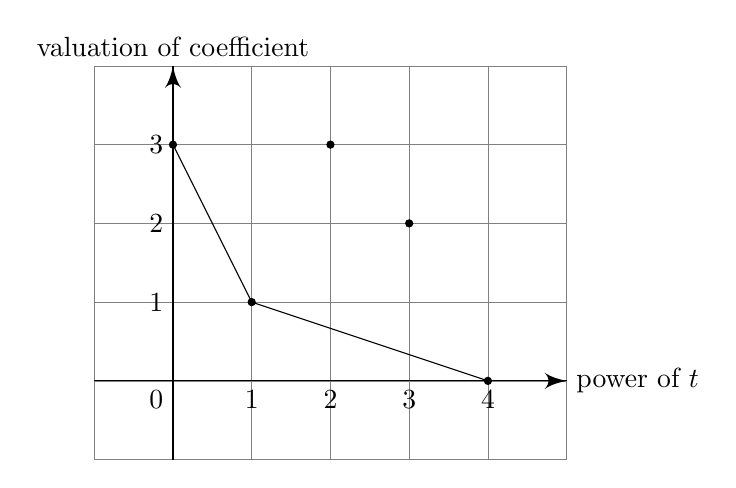
\begin{tikzpicture}
      \draw [step=1,gray, very thin] (-1, 4) grid (5, -1);

      \draw [->] (-1, 0) -- (5, 0) node [right] {power of $t$};
      \draw [->] (0, -1) -- (0, 4) node [above] {valuation of coefficient};

      \node [circ] at (0, 3) {};
      \node [circ] at (1, 1) {};
      \node [circ] at (2, 3) {};
      \node [circ] at (3, 2) {};
      \node [circ] at (4, 0) {};

      \draw (0, 3) -- (1, 1) -- (4, 0);

      \foreach \x in {1,2,3,4} {
        \node at (\x, 0) [below] {$\x$};
      }
      \node at (0, 0) [anchor = north east] {$0$};
      \foreach \y in {1,2,3} {
        \node at (0, \y) [left] {$\y$};
      }
    \end{tikzpicture}
  \end{center}
\end{eg}

\begin{eg}
  Consider $(\Q_2, v_2)$ with the polynomial
  \[
    4t^4 + 5t^3 + \frac{7}{2}t + \frac{9}{2}.
  \]
  Here there is no $t^2$ term, so we simply don't draw anything.
  \begin{center}
    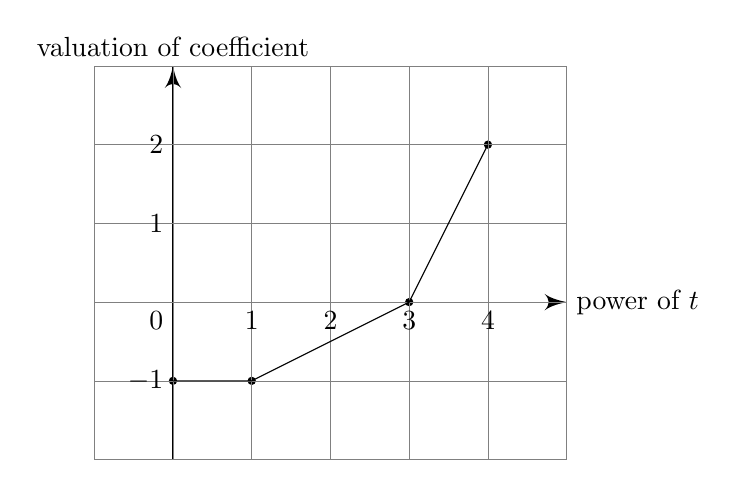
\begin{tikzpicture}
      \draw [->] (-1, 0) -- (5, 0) node [right] {power of $t$};
      \draw [->] (0, -2) -- (0, 3) node [above] {valuation of coefficient};

      \node [circ] at (0, -1) {};
      \node [circ] at (1, -1) {};
      \node [circ] at (3, 0) {};
      \node [circ] at (4, 2) {};

      \draw [step=1,gray, very thin] (-1, 3) grid (5, -2);
      \draw (0, -1) -- (1, -1) -- (3, 0) -- (4, 2);

      \foreach \x in {1,2,3,4} {
        \node at (\x, 0) [below] {$\x$};
      }
      \node at (0, 0) [anchor = north east] {$0$};
      \foreach \y in {-1,1,2} {
        \node at (0, \y) [left] {$\y$};
      }

    \end{tikzpicture}
  \end{center}
\end{eg}

We now go to come up with a formal definition.

\begin{defi}[Lower convex set]\index{lower convex set}
  We say a set $S \subseteq \R^2$ is \emph{lower convex} if
  \begin{enumerate}
    \item Whenever $(x, y) \in S$, then $(x, z) \in S$ for all $z \geq y$.
    \item $S$ is convex.
  \end{enumerate}
\end{defi}
\begin{defi}[Lower convex hull]
  Given any set of points $T \subseteq \R^2$, there is a minimal lower convex set $S \supseteq T$ (by the intersection of all lower convex sets containing $T$ -- this is a non-empty definition because $\R^2$ satisfies the property). This is known as the \term{lower convex hull} of the points.
\end{defi}

\begin{eg}
  The lower convex hull of the points $(0, 3), (1, 1), (2, 3), (3, 2), (4, 0)$ is given by the region denoted below:
   \begin{center}
    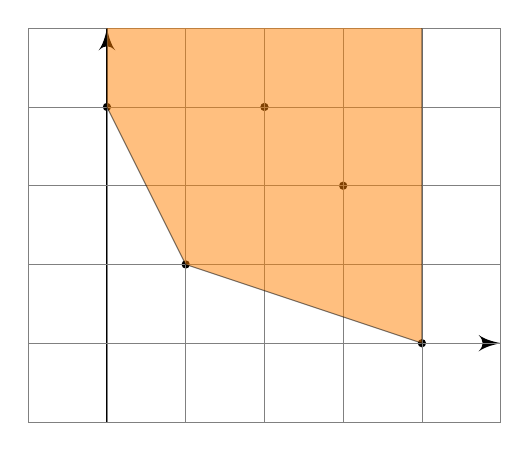
\begin{tikzpicture}
      \draw [->] (-1, 0) -- (5, 0);
      \draw [->] (0, -1) -- (0, 4);

      \node [circ] at (0, 3) {};
      \node [circ] at (1, 1) {};
      \node [circ] at (2, 3) {};
      \node [circ] at (3, 2) {};
      \node [circ] at (4, 0) {};

      \draw [step=1,gray, very thin] (-1, 4) grid (5, -1);
      \draw [fill=morange, opacity=0.5] (0, 4) -- (0, 3) -- (1, 1) -- (4, 0) -- (4, 4);
    \end{tikzpicture}
  \end{center}
\end{eg}

\begin{defi}[Newton polygon]\index{Newton polygon}
  Let $f(x) = a_0 + a_1 x + \cdots + a_n x^n \in K[x]$, where $(K, v)$ is a valued field. Then the \emph{Newton polygon} of $f$ is the lower convex hull of $\{(i, v(a_i)): i = 0, \cdots, n, a_i \not= 0\}$.
\end{defi}
This is the formal definition, so in our first example, the Newton polygon really should be the shaded area shown above, but most of the time, we only care about the lower line.

\begin{defi}[Break points]\index{break points}
  Given a polynomial, the points $(i, v(a_i))$ lying on the boundary of the Newton polygon are known as the \emph{break points}.
\end{defi}

\begin{defi}[Line segment]\index{line segment}
  Given a polynomial, the line segment between two adjacent break points is a \term{line segment}.
\end{defi}

\begin{defi}[Multiplicity/length]\index{multiplicity}\index{length}
  The \emph{length} or \emph{multiplicity} of a line segment is the horizontal length.
\end{defi}

\begin{defi}[Slope]\index{slope}
  The \emph{slope} of a line segment is its slope.
\end{defi}

\begin{eg}
  Consider again $(\Q_2, v_2)$ with the polynomial
  \[
    4t^4 + 5t^3 + \frac{7}{2}t + \frac{9}{2}.
  \]
  \begin{center}
    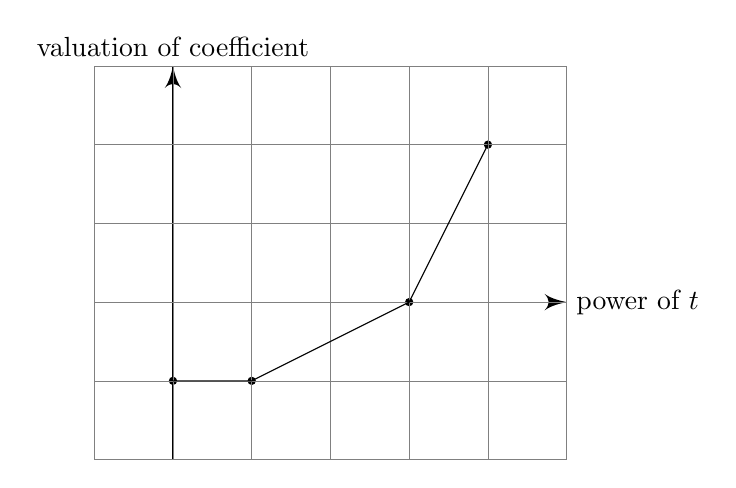
\begin{tikzpicture}
      \draw [->] (-1, 0) -- (5, 0) node [right] {power of $t$};
      \draw [->] (0, -2) -- (0, 3) node [above] {valuation of coefficient};

      \node [circ] at (0, -1) {};
      \node [circ] at (1, -1) {};
      \node [circ] at (3, 0) {};
      \node [circ] at (4, 2) {};

      \draw [step=1,gray, very thin] (-1, 3) grid (5, -2);
      \draw (0, -1) -- (1, -1) -- (3, 0) -- (4, 2);
    \end{tikzpicture}
  \end{center}
  The middle segment has length $2$ and slope $1/2$.
\end{eg}
\begin{eg}
  In the following Newton polygon:
  \begin{center}
    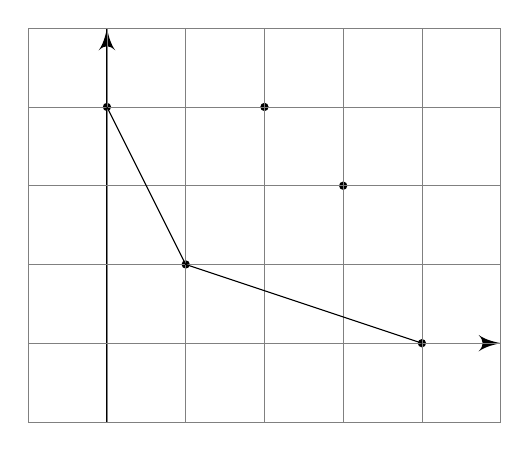
\begin{tikzpicture}
      \draw [->] (-1, 0) -- (5, 0);
      \draw [->] (0, -1) -- (0, 4);

      \node [circ] at (0, 3) {};
      \node [circ] at (1, 1) {};
      \node [circ] at (2, 3) {};
      \node [circ] at (3, 2) {};
      \node [circ] at (4, 0) {};

      \draw [step=1,gray, very thin] (-1, 4) grid (5, -1);
      \draw (0, 3) -- (1, 1) -- (4, 0);
    \end{tikzpicture}
  \end{center}
  The second line segment has length $3$ and slope $-\frac{1}{3}$.
\end{eg}

It turns out the Newton polygon tells us something about the roots of the polynomial.
\begin{thm}
  Let $K$ be complete valued field, and $v$ the valuation on $K$. We let
  \[
    f(x) = a_0 + a_1 x + \cdots + a_n x^n \in K[x].
  \]
  Let $L$ be the splitting field of $f$ over $K$, equipped with the unique extension $w$ of $v$.

  If $(r, v(a_r)) \to (s, v(a_s))$ is a line segment of the Newton polygon of $f$ with slope $-m \in \R$, then $f$ has precisely $s - r$ roots of valuation $m$.
\end{thm}
Note that by lower convexity, there can be at most one line segment for each slope. So this theorem makes sense.

\begin{proof}
  Dividing by $a_n$ only shifts the polygon vertically, so we may wlog $a_n = 1$. We number the roots of $f$ such that
  \begin{align*}
    w(\alpha_1) &= \cdots = w(\alpha_{s_1}) = w_1\\
    w(\alpha_{s_1 + 1}) &= \cdots = w(\alpha_{s_2}) = w_2\\
    &\vdots\\
    w(\alpha_{s_t}) &= \cdots = w(\alpha_n) = w_{t + 1},
  \end{align*}
  where we have
  \[
    w_1 < w_2 < \cdots < w_{t + 1}.
  \]
  Then we know
  \begin{align*}
    v(a_n) &= v(1) = 0\\
    v(a_{n - 1}) &= w\left(\sum \alpha_i\right) \geq \min_i w(\alpha_i) = w_1\\
    v(a_{n - 2}) &= w\left(\sum \alpha_i\alpha_j\right) \geq \min_{i \not= j} w(\alpha_i \alpha_j) = 2 m_1\\
    &\vdots\\
    v(a_{n - s_1}) &= w\left(\sum_{i_1\not=\ldots \not=i_{s_1}} \alpha_{i_1 \ldots \alpha_{i_{s_1}}}\right) = \min w(\alpha_{i_1}\cdots\alpha_{i_{s_1}}) = s_1 m_1.
  \end{align*}
  It is important that in the last one, we have equality, not an inequality, because there is one term in the sum whose valuation is less than all the others.

  We can then continue to get
  \[
    v(\alpha_{n - s_1 - 1}) \geq \min w(\alpha_{i_1} \cdots \alpha_{i_{s_1 + 1}}) = s_1 m_1 + m_2,
  \]
  until we reach
  \[
    v(\alpha_{n - s_1 - s_2}) = s_1 m_1 + (s_2 - s_1) m_2.
  \]
  We keep going on.

  We draw the Newton polygon.
  \begin{center}
    \begin{tikzpicture}
      \draw [->] (-1, 0) -- (8, 0);
      \draw [->] (0, -2) -- (0, 2);

      \node [circ] at (7, 0) {};
      \node [above] at (7, 0) {$(n, 0)$};

      \node [circ] at (5, -1) {};
      \node [right] at (5, -1) {$(n - s_1, s_1 m_1)$};

      \node [circ] at (3, -1.5) {};
      \node [below] at (3, -1.5) {$(n - s_1 - s_2, s_1 m_1 + (s_2 - s_1) m_1)$};

      \node at (2, -1.5) {$\cdots$};

      \draw (7, 0) -- (5, -1) -- (3, -1.5);
    \end{tikzpicture}
  \end{center}
  We don't know where exactly the other points are, but the inequalities imply that the $(i, v(a_i))$ are above the lines drawn. So this is the Newton polygon.

  Counting from the right, the first line segment has length $n - (n - s_1) = s_1$ and slope
  \[
    \frac{0 - s_1 m_1}{n - (n - s_1)} = -m_1.
  \]
  In general, the $k$th segment has length $(n - s_{k - 1}) - (n - s_k) = s_k - s_{k - 1}$, and slope
  \begin{align*}
    &\frac{\left(s_1 m_1 + \sum_{i = 1}^{k - 2} (s_{i + 1} - s_i) m_{i + 1}\right) - \left(s_1 m_1 + \sum_{i = 1}^{k - 1} (s_{i + 1} - s_i) m_{i + 1}\right)}{s_k - s_{k - 1}} \\
    ={}& \frac{-(s_k - s_{k - 1})m_k}{s_k - s_{k - 1}} = - m_k.
  \end{align*}
  and the others follow similarly.
\end{proof}

\begin{cor}
  If $f$ is irreducible, then the Newton polygon has a single line segment.
\end{cor}

\begin{proof}
  We need to show that all roots have the same valuation. Let $\alpha, \beta$ be in the splitting field $L$. Then there is some $\sigma \in \Aut(L/K)$ such that $\sigma(\alpha) = \beta$. Then $w(\alpha) = w(\sigma(\alpha)) = \beta$. So done.
\end{proof}

Note that Eisenstein's criterion is a (partial) converse to this!

\section{Discretely valued fields}
We are now going to further specialize. While a valued field already has some nice properties, we can't really say much more about them without knowing much about their valuations.

Recall our previous two examples of valued fields: $\Q_p$ and $\F_p((T))$. The valuations had the special property that they take values in $\Z$. Such fields are known as \emph{discretely valued fields}.

\begin{defi}[Discretely valued field]\index{discretely valued field}\index{valued field!discretely}\index{DVF}
  Let $K$ be a valued field with valuation $v$. We say $K$ is a \emph{discretely valued field} (DVF) if $v(k^\times) \subseteq \R$ is a discrete subgroup of $\R$, ie. $v(k^\times)$ is infinite cyclic.
\end{defi}
Note that we do not require the image to be exactly $\Z \subseteq \R$. So we allow scaled versions of the valuation. This is useful because the property of mapping to $\Z$ is not preserved under field extensions in general, as we will later see. We will call those that do land in $\Z$ \emph{normalized valuations}.

\begin{defi}[Normalized valuation]\index{normalized valuation}\index{valuation!normalized}
  Let $K$ be a DVF. The \emph{normalized valuation} $V_K$ on $K$ is the unique valuation on $K$ in the given equivalence class of valuations whose image is $\Z$.
\end{defi}

Note that the normalized valuation does not give us a preferred choice of absolute value, since to obtain an absolute value, we still have to arbitrarily pick the base $c > 1$ to define $|x| = c^{-v(x)}$.

\begin{defi}[Uniformizer]\index{uniformizer}
  Let $K$ be a discrete valued field. We say $\pi \in K$ is \emph{uniformizer} if $v(\pi) > 0$ and $v(\pi)$ generates $v(k^\times)$ (iff $v(\pi)$ has minimal positive valuation).
\end{defi}
So with a normalized valuation, we have $v_K(\pi)$.

\begin{eg}
  The usual valuation on $\Q_p$ is normalized, and so is the usual valuation on $k((T))$. $p$ is a uniformizer for $\Q_p$ and $t$ is a uniformizer for $k((T))$.
\end{eg}

The kinds of fields we will be interested are \emph{local fields}. The definition we have here might seem rather ad hoc. This is just one of the many equivalent characterizations of a local field, and the one we pick here is the easiest to state.
\begin{defi}[Local field]\index{local field}
  A complete discretely valued field with a finite residue field is called a \emph{local field}.
\end{defi}

\begin{eg}
  $\Q$ and $\Q_p$ with $v_p$ are both discretely valued fields, and $\Q_p$ is a local field. $p$ is a uniformizer.
\end{eg}

\begin{eg}
  The Laurent series field $k((T))$ with valuation
  \[
    v\left(\sum a_n T^n\right) = \inf\{n: a_n \not= 0\}
  \]
  is a discrete valued field, and is a local field if and only if $k$ is finite field, as the residue field is exactly $k$. We have
  \[
    \mathcal{O}_{k((T))} = k[[T]] = \left\{\sum_{n = 0}^\infty a_n T^n: a_n \in k\right\}.
  \]
  Here $T$ is a uniformizer.
\end{eg}

These discretely valued field are pretty much like the $p$-adic numbers.
\begin{prop}
  Let $K$ be a discretely valued field with uniformizer $\pi$. Let $S \subseteq \mathcal{O}_K$ be a set of coset representatives of $\mathcal{O}_k/\mathfrak{m}_k = k_K$ containing $0$. Then
  \begin{enumerate}
    \item The non-zero ideals of $\mathcal{O}_K$ are $\pi^n \mathcal{O}_K$ for $n \geq 0$.
    \item The ring $\mathcal{O}_K$ is a PID with unique prime $\pi$ (up to units), and $\mathfrak{m}_K = \pi\mathcal{O}_K$.
    \item The topology on $\mathcal{O}_K$ induced by the absolute value is the $\pi$-adic topology.
    \item If $K$ is complete, then $\mathcal{O}_K$ is $\pi$-adically complete
    \item if $K$ is complete, then any $x \in K$ can be written uniquely as
      \[
        x = \sum_{n \gg -\infty}^\infty a_n \pi^n,
      \]
      where $a_n \in S$, and
      \[
        |x| = |\pi|^{-\inf\{n: a_n \not= 0\}}.
      \]
    \item The completion $\hat{K}$ is also discretely valued and $\pi$ is a uniformizer, and moreover the natural map
      \[
        \begin{tikzcd}
          \displaystyle\frac{\mathcal{O}_k}{\pi^n \mathcal{O}_k} \ar[r, "\sim"] & \displaystyle\frac{\mathcal{O}_{\hat{K}}}{\pi^n \mathcal{O}_{\hat{K}}}
        \end{tikzcd}
      \]
      is an isomorphism.
  \end{enumerate}
\end{prop}

\begin{proof}
  The same as for $\Q_p$ and $\Z_p$, with $\pi$ instead of $p$.
\end{proof}

\begin{prop}
  Let $K$ be a discretely valued field. Then $K$ is a local field iff $\mathcal{O}_K$ is compact.
\end{prop}

\begin{proof}
  If $\mathcal{O}_K$ is compact, then $\pi^{-n}\mathcal{O}_K$ is compact for all $n \geq 0$ (where $\pi$ is the uniformizer), and in particular complete. So
  \[
    K = \bigcup_{n \geq 0}^\infty \pi^{-n} \mathcal{O}_K
  \]
  is complete, as this is an increasing union, and Cauchy sequences are bounded. Also, we know the quotient map $\mathcal{O}_K \to k_K$ is continuous when $k_K$ is given the discrete topology, by definition of the $\pi$-adic topology. So $k_K$ is compact and discrete, hence finite.

  In the other direction, if $K$ is local, then we know $\mathcal{O}_K/\pi^n \mathcal{O}_K$ is finite for all $n \geq 0$ (by induction and finiteness of $k_K$). We let $(x_i)$ be a sequence in $\mathcal{O}_K$. Then by finiteness of $\mathcal{O}_K/\pi \mathcal{O}_K$, there is a subsequence $(x_{1, i})$ which is constant modulo $\pi$. We keep going, choosing a subsequence $(x_{n + 1, i})$ of $(x_{n_i})$ such that $(x_{n + 1, i})$ is constant modulo $\pi^{n + 1}$. Then $(x_{i, i})_{i = 1}^\infty$ converges, since it is Cauchy as
  \[
    |x_{ii} - x_{jj}| \leq |\pi|^j
  \]
  for $j \leq i$. So $\mathcal{O}_K$ is sequentially compact, hence compact.
\end{proof}

Now the valuation ring $\mathcal{O}_K$ inherits a valuation from $K$, and this gives it a structure of a \emph{discrete valuation ring}. We will define a discrete valuation ring in a funny way, but there are many equivalent definitions that we will not list.

\begin{defi}[Discrete valuation ring]\index{discrete valuation ring}\index{DVR}
  A ring $R$ is called a \emph{discrete valuation ring} (DVR) if it is a PID with a unique prime element up to units.
\end{defi}

\begin{prop}
  $R$ is a DVR iff $R \cong \mathcal{O}_K$ for some DVF $K$.
\end{prop}

\begin{proof}
  We have already seen that valuation rings of discrete valuation fields are DVRs. In the other direction, let $R$ be a DVR, and $\pi$ a prime. Let $x \in \R \setminus \{0\}$. Then we can find a unique unit $u \in R^\times$ and $n \in \Z_{\geq 0}$ such that $x = \pi^n u$ (say, by unique factorization of PIDs). We define
  \[
    v(x) =
    \begin{cases}
      n & x \not= 0\\
      \infty & x = 0
    \end{cases}
  \]
  This is then a discrete valuation of $R$. This extends uniquely to the field of fractions $K$. It remains to show that $R = \mathcal{O}_K$. First note that
  \[
    K = R\left[\frac{1}{\pi}\right].
  \]
  This is since any non-zero element in $R\left[\frac{1}{\pi}\right]$ looks like $\pi^n u, u \in R^\times, n \in \Z$, and is already invertible. So it must be the field of fractions. Then we have
  \[
    v(\pi^n u) = n \in \Z_{\geq 0} \Longleftrightarrow \pi^n u \in R.
  \]
  So we have $R = \mathcal{O}_K$.
\end{proof}

Now recall our two ``standard'' examples of valued fields --- $\F_p((T))$ and $\Q_p$. Both of their residue fields are $\F_p$, and in particular has characteristic $p$. However, $\F_p((T))$ itself is \emph{also} of characteristic $p$, while $\Q_p$ has characteristic $0$. It would thus be helpful to split these into two different cases:

\begin{defi}[Equal and mixed characteristic]\index{equal characteristic}\index{mixed characteristic}
  Let $K$ be a valued field with residue field $k_K$. Then $K$ has \emph{equal characteristic} if
  \[
    \Char K = \Char k_K.
  \]
  Otherwise, we have $K$ has \emph{mixed characteristic}.
\end{defi}
If $K$ has mixed characteristic, then necessarily $\Char K = 0$, and $\Char k_K > 0$.

\begin{eg}
  $\Q_p$ has mixed characteristic, since $\Char \Q_p = 0$ but $\Char k_{\Q_p} = \Z/p\Z = p$.
\end{eg}

We will also need the following definition:
\begin{defi}[Perfect ring]\index{perfect ring}
  Let $R$ be a ring of characteristic $p$. We say $R$ is \emph{perfect} if the Frobenius map $x \mapsto x^p$ is an automorphism of $R$, ie. every element of $R$ has a $p$th root.
\end{defi}

\begin{fact}
  Let $F$ be a field of characteristic $p$. If $F$ is perfect if and only if every finite extension of $F$ is separable.
\end{fact}

\begin{eg}
  $\F_q$ is perfect for every $q = p^n$.
\end{eg}

\subsection{\texorpdfstring{Teichm\"uller}{Teichmuller} lifts}
Take our favorite discretely valued ring $\Z_p$. This is $p$-adically complete, so we can write each element as
\[
  x = a_0 + a_1 p + a_2 p^2 + \cdots,
\]
where each $a_i$ is in $\{0, 1, \cdots, p - 1\}$. The reason this works is that $0, 1, \cdots, p - 1$ are coset representatives of the ring $\Z_p/p \Z_p \cong \Z/p\Z$. While these coset representatives might feel like a ``natural'' thing to do in this context, this is because we have implicitly identified with $\Z_p/p\Z_p \cong \Z/p\Z$ as a particular subset of $\Z \subseteq \Z_p$. However, this identification respects effectively no algebraic structure at all. For example, we cannot multiplying the cosets simply by multiplying the representatives as elements of $\Z_p$, because, say, $(p - 1)^2 = p^2 - 2p + 1$, which is not $1$. So this is actually quite bad, at least theoretically.

It turns out that we can actually construct ``natural'' lifts in a very general scenario.
\begin{lemma}
  Let $R$ be a ring, and let $x \in R$. Assume that $R$ is $x$-adically complete and that $R/xR$ is perfect of characteristic $p$. Then there is a unique map $[-]: R/xR \to R$ such that
  \[
    [a] \equiv a \mod x
  \]
  and
  \[
    [ab] = [a][b].
  \]
  for all $a, b \in R/xR$. Moreover, if $R$ has characteristic $p$, then $[-]$ is a ring homomorphism.
\end{lemma}

\begin{defi}[Teichm\"uller map]\index{Teichm\"uller map}\index{Teichm\"uller lift}\index{Teichm\"uller representative}
  The map $[-]: R/xR \to R$ is called the \emph{Teichm\:uller map}. $[x]$ is called the \emph{Teichm\"uller lift} or \emph{representative} of $x$.
\end{defi}

The idea of the proof is as follows: suppose we have an $a \in R/xR$. If we randomly picked a lift $\alpha$, then chances are it would be a pretty ``bad'' choice, since any two such choices can differ by a multiple of $x$.

Suppose we instead lifted a $p$th root of $a$ to $R$, and then take the $p$th power of it. We claim that this is a better way of picking a lift. Suppose we have picked two lifts of $a^{p^{-1}}$, say, $\alpha_1$ and $\alpha_1'$. Then $\alpha_1' = xc + \alpha_1$ for some $c$. So we have
\[
  (\alpha_1')^p - \alpha_1^p = \alpha_1^p + pxc + O(x^2) - \alpha_1^p = pxc + O(x^2),
\]
where we abuse notation and write $O(x^2)$ to mean terms that are multiples of $x^2$.

We now recall that $R/xR$ has characteristic $p$, so $p \in xR$. Thus in fact $pxc = O(x^2)$. So we have
\[
  (\alpha_1')^p - \alpha_1^p = O(x^2).
\]
So while the lift is still arbitrary, any two arbitrary choices can differ by at most $x^2$. Alternatively, our lift is now a well-defined element of $R/x^2 R$.

We can, of course, do better. We can lift the $p^2$th root of $a$ to $R$, then take the $p^2$th power of it. Now any two lifts can differ by at most $O(x^3)$. More generally, we can try to lift the $p^n$th root of $a$, then take the $p^n$th power of it. We keep picking a higher and higher $n$, take the limit, and hopefully get something useful out!

\begin{proof}
  Let $a \in R/xR$. For each $n$, there is a unique $a^{p^{-n}} \in R/xR$. We lift this arbitrarily to some $\alpha_n \in R$ such that
  \[
    \alpha_n \equiv a^{p^{-n}} \mod x.
  \]
  We define
  \[
    \beta_n = \alpha_n^{p^n}.
  \]
  The claim is that
  \[
    [a] = \lim_{n \to \infty}\beta_n
  \]
  exists and is independent of the choices.

  Note that if the limit exists no matter how we choose the $\alpha_n$, then it must be independent of the choices. Indeed, if we had choices $\beta_n$ and $\beta_n'$, then $\beta_1, \beta_2', \beta_3, \beta_4', \beta_5, \beta_6', \cdots$ is also a respectable choice of lifts, and thus must converge. So $\beta_n$ and $\beta_n'$ must have the same limit.

  Since the ring is $x$-adically complete and is discretely valued, to show the limit exists, it suffices to show that $\beta_{n + 1} - \beta_n \to 0$ $x$-adically. Indeed, we have
  \[
    \beta_{n + 1} - \beta_n = (\alpha_{n + 1}^p)^{p^n} - \alpha_n^{p^n}.
  \]
  We now notice that
  \[
    \alpha_{n + 1}^p \equiv (a^{p^{-n - 1}})^p = a^{p^{-n}} \equiv \alpha_n \mod x.
  \]
  Using the fact that $R/xR$ has characteristic $p$, so that $p \in xR$, the binomial theorem give
  \[
    (\alpha_{n + 1}^p)^{p^n} \equiv \alpha_n^{p^n} \mod x^{n + 1}.
  \]
  So $\beta_{n + 1} - \beta_n \in x^{n + 1} R$. So $\lim \beta_n$ exists.

  To see $[a] = a\mod x$, we just have to note that
  \[
    \lim_{n \to \infty} \alpha_n^{p^n} \equiv \lim_{n \to \infty} (a^{p^{-n}})^{p^n} = \lim a = a \mod x.
  \]
  (here we are using the fact that the map $R \to R/xR$ is continuous when $R$ is given the $x$-adic topology and $R/xR$ is given the discrete topology)

  The remaining properties then follow trivially from the uniqueness of the above limit.

  For multiplicativity, if we have another element $b \in R/xR$, with $\gamma_n \in R$ lifting $b^{p^{-n}}$ for all $n$, then $\alpha_n \gamma_n$ lifts $(ab)^{p^{-n}}$. So
  \[
    [ab] = \lim\alpha_n^{p^n} \gamma_n^{p^n} = \lim \alpha_n^{p^n} \lim \gamma_n^{p^n} = [a][b].
  \]
  If $R$ has characteristic $p$, then $\alpha_n + \gamma_n$ lifts $a^{p^{-n}} + b^{p^{-n}} = (a + b)^{p^{-n}}$. So
  \[
    [a + b] = \lim (\alpha_n + \gamma_n)^{p^n} = \lim \alpha_n^{p^n} + \lim \gamma_n^{p^n} = [a] + [b].
  \]
  Since $1$ is a lift of $1$ and $0$ is a lift of $0$, it follows that this is a ring homomorphism.

  Finally, to show uniqueness, suppose $\phi: R/xR \to R$ is a map with these properties. Then we note that $\phi(a^{p^{-n}}) \equiv a^{p^{-n}} \mod x$, and is thus a valid choice of $\alpha_n$. So we have
  \[
    [a] = \lim_{n \to \infty} \phi(a^{p^{-n}})^{p^n} = \lim \phi(a) = \phi(a).
  \]
\end{proof}

\begin{eg}
  Let $R = \Z_p$ and $x = p$. Then $[-]: \F_p \to \Z_p$ satisfies
  \[
    [x]^{p - 1} = [x^{p - 1}] = [1] = 1.
  \]
  So the image of $[x]$ must be the unique $p - 1$th root of unity lifting $x$ (recall we proved their existence via Hensel's lemma).
\end{eg}

When proving theorems about these rings, the Teichm\"uller lifts would be very handy and natural things to use. However, when we want to do actual computations, there is absolutely no reason why these would be easier!

As an application, we can prove the following characterization of equal characteristic complete DVF's.
\begin{thm}
  Let $K$ be a complete discretely valued field of equal characteristic $p$, and assume that $k_K$ is perfect. Then $K \cong k_K((T))$.
\end{thm}

\begin{proof}
  Let $K$ be a complete DVF. Since every DVF the field of fractions of its valuation ring, it suffices to prove that $\mathcal{O}_K \cong k_K[[T]]$. We know $\mathcal{O}_K$ has characteristic $p$. So $[-]: k_K \to \mathcal{O}_K$ is an injective ring homomorphism. We choose a uniformizer $\pi \in \mathcal{O}_K$, and define
  \[
    k_K[[T]] \to \mathcal{O}_K
  \]
  by
  \[
    \sum_{n = 0}^\infty a_n T^n \mapsto \sum_{n = 0}^\infty [a_n] \pi^n.
  \]
  Then this is a ring homomorphism since $[-]$ is. The bijectivity follows from property (v) in our list of properties of complete DVF's.
\end{proof}

\begin{cor}
  Let $K$ be a local field of equal characteristic $p$. Then $k_K \cong \F_q$ for some $q$ a power of $p$, and $K \cong F_q((T))$.
\end{cor}

\subsection{Witt vectors*}
We are now going to look at the mixed characteristic analogue of this result. We want something that allows us to go from characteristic $p$ to characteristic $0$. This is known as \emph{Witt vectors}, which is non-examinable.

We start with the notion of a \emph{strict $p$-ring}. Roughly this is a ring that satisfies all the good properties whose name has the word ``$p$'' in it.
\begin{defi}[Strict $p$-ring]\index{strict $p$-ring}
  Let $A$ be a ring. A is called a \emph{strict $p$-ring} if it is $p$-torsion free, $p$-adically complete, and $A/pA$ is a perfect ring.
\end{defi}

Note that a strict $p$-ring in particular satisfies the conditions for the Teichm\"uller lift to exist, for $x = p$.
\begin{eg}
  $\Z_p$ is a strict $p$-ring.
\end{eg}

The next example we are going to construct is more complicated. This is in some sense a generalization of the usual polynomial rings $\Z[x_1, \cdots, x_n]$, or more generally,
\[
  \Z[x_i \mid i \in I],
\]
for $I$ possibly infinite. To construct the ``free'' strict $p$-ring, after adding all these variables $x_i$, to make it a strict $p$-ring, we also need to add their $p$th roots, and the $p^2$th roots etc, and then take the $p$-adic completion, and hope for the best.

\begin{eg}
  Let $X = \{x_i: i \in I\}$ be a set. Let
  \[
    B = \Z[x_i^{p^{-\infty}}\mid i \in I] = \bigcup_{n = 0}^\infty \Z[x_i^{p^{-n}}\mid i \in I].
  \]
  Here the union on the right is taken by treating
  \[
    \Z[x_i \mid i \in I] \subseteq \Z [x_i^{p^{-1}} \mid i \in I] \subseteq \cdots
  \]
  in the natural way.

  We let $A$ be the $p$-adic completion of $B$. We claim that $A$ is a strict $p$-ring and $A/pA \cong \F_p[x_i^{p^{-\infty}}\mid i \in I]$.

  Indeed, we see that $B$ is $p$-torsion free. By Exercise 13 on Sheet 1, we know $A$ is $p$-adically complete and torsion free. Moreover,
  \[
    A/pA \cong B/pB \cong \F_p[x_i^{p^{-\infty}}\mid i \in I],
  \]
  which is perfect since every element has a $p$-th root. % why % definition
\end{eg}

If $A$ is a strict $p$-ring, then we know that we have a Teichm\"uller map
\[
  [-]: A/pA \to A,
\]
\begin{lemma}
  Let $A$ be a strict $p$-ring. Then any element of $A$ can be written uniquely as
  \[
    a = \sum_{n = 0}^\infty [a_n] p^n,
  \]
  for a \emph{unique} $a_n \in A/pA$.
\end{lemma}

\begin{proof}
  We recursively construct the $a_n$ by
  \begin{align*}
    a_0 &= a \pmod p\\
    a_1 &\equiv p^{-1}(a - [a_0]) \pmod p\\
    &\vdots
  \end{align*}
\end{proof}

\begin{lemma}
  Let $A$ and $B$ be strict $p$-rings and let $f: A/pA \to B/pB$ be a ring homomorphism. Then there is a unique homomorphism $F: A \to B$ such that $f = F \bmod p$, given by
  \[
    F\left(\sum [a_n]p^n\right) = \sum [f(a_n)] p^n.
  \]
\end{lemma}

\begin{proof}[Proof sketch]
  We define $F$ by the given formula and check that it works. First of all, by the formula, $F$ is continuous is $p$-adically continuous, and the key thing is to check that it is additive (which is slightly messy). Multiplicativity then follows formally from the continuity and additivity.

  To show uniqueness, suppose that we have some $\psi$ lifting $f$. Then $\psi(p) = p$. So $\psi$ is $p$-adically continuous. So it suffices to show that $\psi([a]) = [\psi(a)]$.

  We take $\alpha_n \in A$ lifting $a^{p^{-n}} \in A/pA$. Then $\psi(\alpha_n)$ lifts $f(a)^{p^{-n}}$. So
  \[
    \psi([a]) = \lim \psi(\alpha_n^{p^{-n}}) = \lim \psi(\alpha_n)^{p^n} = [f(a)].
  \]
  So done.
\end{proof}

There is a generalization of this result which we shall not prove:
\begin{prop}
  Let $A$ be a strict $p$-ring and $B$ be a ring with an element $x$ such that $B$ is $x$-adically complete and $B/xB$ is perfect of characteristic $p$. If $f: A/pA \to B/xB$ is a ring homomorphism. Then there exists a ring homomorphism $F: A \to B$ with $f = F \mod x$, ie. the following diagram commutes:
  \[
    \begin{tikzcd}
      A \ar[r, "F"] \ar[d] & B \ar[d]\\
      A/pA \ar[r, "f"] & B/xB
    \end{tikzcd}.
  \]
\end{prop}

We can now state the main theorem about strict $p$-rings.

\begin{thm}
  Let $R$ be a perfect ring. Then there is a unique (up to isomorphism) strict $p$-ring $W(B)$\index{$W(R)$} called the \term{Witt vector}\emph{s} of $R$ such that $W(R)/p W(R) \cong R$.

  Moreover, for any other perfect ring $R$, the reduction mod $p$ map gives a bijection
  \[
    \begin{tikzcd}
      \Hom_{\mathrm{Ring}}(W(R), W(R')) \ar[r, "\sim"] & \Hom_{\mathrm{Ring}}(R, R')
    \end{tikzcd}.
  \]
\end{thm}

\begin{proof}[Proof sketch]
  If $W(R)$ and $W(R')$ are such strict $p$-rings, then the second part follows from the previous lemma. Indeed, if $C$ is a strict $p$-ring with $C/pC \cong R \cong W(R)/pW(R)$, then the isomorphism $\bar{\alpha}: W(R)/pW(R) \to C/pC$ and its inverse $\bar{\alpha}^{-1}$ have unique lifts $\gamma: W(R) \to C$ and $\gamma^{-1}: C \to W(R)$, and these are inverses by uniqueness of lifts.

  To show existence, let $R$ be a perfect ring. We form
  \begin{align*}
    \F_p[x_r^{p^{-\infty}}\mid r \in R] &\to R\\
    x_r&\mapsto r
  \end{align*}
  Then we know that the $p$-adic completion of $\Z[x_r^{p^{-\infty}}\mid r \in R]$, written $A$, is a strict $p$-ring with
  \[
    A/pA \cong \F_p[x_r^{p^{-\infty}}\mid r \in R].
  \]
  We write
  \[
    I = \ker(\F_p[x_r^{p^{-\infty}}\mid r \in R] \to R).
  \]
  Then define
  \[
    J = \left\{\sum_{n = 0}^\infty [a_k] p^n \in A: a_n \in I\text{ for all $n$}\right\}.
  \]
  This turns out to be an ideal.

  We put $W(R) = A/J$. We can then painfully check that this has all the required properties. For example, if
  \[
    x = \sum_{n = 0}^\infty [a_n] p^n \in A,
  \]
  and
  \[
    px = \sum_{n = 0}^\infty [a_n] p^{n + 1} \in J,
  \]
  then by definition of $J$, we know $[a_n] \in I$. So $x \in J$. So $W(R)/J$ is $p$-torsion free. By a similar calculation, one checks that
  \[
    \bigcap_{n = 0}^\infty p^n W(R) = \{0\}.
  \]
  This implies that $W(R)$ injects to its $p$-adic completion. Using that $A$ is $p$-adically complete, one checks the surjectivity by hand.

  Also, we have
  \[
    \frac{W(R)}{p W(R)} \cong \frac{A}{J + pA}.
  \]
  But we know
  \[
    J + pA = \left\{\sum_n [a_n] p^n \mid a_0 \in I\right\}.
  \]
  So we have
  \[
    \frac{W(R)}{pW(R)} \cong \frac{\F_p[x_r^{p^{-\infty}}\mid r \in R]}{I} \cong R.
  \]
  So we know that $W(R)$ is a strict $p$-ring.
\end{proof}

\begin{eg}
  $W(\F_p) = \Z_p$, since $\Z_p$ satisfies all the properties $W(\F_p)$ is supposed to satisfy.
\end{eg}

\begin{prop}
  A complete DVR $A$ of mixed characteristic with perfect residue field and such that $p$ is a uniformizer is the same as a strict $p$-ring $A$ such that $A/pA$ is a field.
\end{prop}

\begin{proof}
  Let $A$ be a complete DVR such that $p$ is a uniformizer and $A/pA$ is perfect. Then $A$ is $p$-torsion free, as $A$ is an integral domain of characteristic $0$. Since it is also $p$-adically complete, it is a strict $p$-ring.

  Conversely, if $A$ is a strict $p$-ring, and $A/pA$ is a field, then we have $A^\times \subseteq A \setminus pA$, and we claim that $A^\times = A \setminus pA$. Let
  \[
    x = \sum_{n = 0}^\infty [x_n] p^n
  \]
  with $x_0 \not= 0$, ie. $x \not\in pA$. We want to show that $x$ is a unit. Since $A/pA$ is a field, we can multiply by $[x_0^{-1}]$, so we may wlog $x_0 = 1$. Then $x = 1 - py$ for some $y \in A$. So we can invert this with a geometric series
  \[
    x^{-1} = \sum_{n = 0}^\infty p^n y^n.
  \]
  So $x$ is a unit. Now, looking at Teichm\"uller expansions and factoring out multiple of $p$, any non-zero element $z$ can be written as $p^n u$ for a unique $n \geq \Z_{\geq 0}$ and $u \in A^\times$. Then we have
  \[
    v(z) =
    \begin{cases}
      n & z \not= 0\\
      \infty & z = 0
    \end{cases}
  \]
  is a discrete valuation on $A$.
\end{proof}

\begin{defi}[Absolute ramification index]\index{absolute ramification index}
  Let $R$ be a DVR with mixed characteristic $p$ with normalized valuation $v_R$. The integer $v_R(p)$ is called the \emph{absolute ramification index} of $R$.
\end{defi}

\begin{cor}
  Let $R$ be a complete DVR of mixed characteristic with absolute ramification index $1$ and perfect residue field $k$. Then $R \cong W(k)$.
\end{cor}

\begin{proof}
  Having absolute ramification index $1$ is the same as saying $p$ is a uniformizer. So $R$ is a strict $p$-ring with $R/pR \cong k$. By uniqueness of the Witt vector, we know $R \cong W(k)$.
\end{proof}

\begin{thm}
  Let $R$ be a complete DVR of mixed characteristic $p$ with a perfect residue field $k$ and uniformizer $\pi$. Then $R$ is finite over $W(k)$.
\end{thm}

\begin{proof}
  We need to first exhibit $W(k)$ as a subring of $R$. We know that $\id: k \to k$ lifts to a homomorphism $W(k) \to R$. The kernel is a prime ideal because $R$ is an integral domain. So it is either $0$ or $p W(k)$. But $R$ has characteristic $0$. So it can't be $pW(k)$. So this must be an injection.

  Let $e$ be the absolute ramification index of $R$. We want to prove that
  \[
    R = \bigoplus_{i = 0}^{e - 1} \pi^i W(k).
  \]
  Looking at valuations, one sees that $1, \pi, \pi, \cdots, \pi^{e - 1}$ are linearly independent over $W(k)$. So we can form
  \[
    M = \bigoplus_{i = 0}^{e - 1} \pi^i W(k) \subseteq R.
  \]
  We consider $R/pR$. Looking at Teichm\"uller expansions
  \[
    \sum_{n = 0}^\infty [x_n] \pi^n \equiv \sum_{n = 0}^{e - 1} [x_n]\pi^n \mod pR,
  \]
  we see that $1, \pi, \cdots, \pi^{e - 1}$ generate $R/pR$ as $W(k)$-modules (all the Teichm\"uller lifts live in $W(k)$). Therefore $R = M + pR$. We iterate to get
  \[
    R = M + p(M + pR) = M + p^2 r = \cdots = M + p^m R
  \]
  for all $m \geq 1$. So $M$ is dense in $R$. But $M$ is also $p$-adically complete, hence closed in $R$. So $M = R$.
\end{proof}

The important statement to take away is
\begin{cor}
  Let $K$ be a mixed characteristic local field. Then $K$ is a finite extension of $\Q_p$.
\end{cor}

\begin{proof}
  Let $\F_q$ be the residue field of $K$. Then $\mathcal{O}_K$ is finite over $W(\F_q)$ by the previous theorem. So it suffices to show that $W(\F_q)$ is finite over $W(\F_p) = \Z_p$. Again the inclusion $\F_p \subseteq \F_q$ gives an injection $W(\F_p) \hookrightarrow W(\F_q)$. Write $q = p^d$, and let $x_1, \cdots, x_d \in W(F_q)$ be lifts of an $\F_p$-bases of $\F_q$.. Then we have
  \[
    W(\F_q) = \bigoplus_{i = 1}^d x_d \Z_p + p W(\F_q),
  \]
  and then argue as in the end of the previous theorem to get
  \[
    W(\F_q) = \bigoplus_{i = 1}^d x_d \Z_p. \qedhere
  \]
\end{proof}

\section{Some \texorpdfstring{$p$}{p}-adic analysis}
We are now going to do some fun things that is not really related to the course. In ``normal'' analysis, the applied mathematicians hold the belief that every function can be written as a power series
\[
  f(x) = \sum_{n = 0}^\infty a_n x^n.
\]
When we move on to $p$-adic numbers, we do not get such a power series expansion. However, we obtain an analogous result using binomial coefficients.

Before that, we have a quick look at our familiar functions $\exp$ and $\log$, which we shall continue to define as a power series:
\[
  \exp(x) = \sum_{n = 0}^\infty \frac{x^n}{n!},\quad \log(1 + x) = \sum_{n = 1}^\infty (-1)^{n - 1}\frac{x^n}{n}
\]
The domain will no longer be all of the field. Instead, we have the following result:
\begin{prop}
  Let $K$ be a complete valued field with an absolute value $|\ph|$ and assume that $K \supseteq \Q_p$ and $|\ph|$ restricts to the usual $p$-adic norm on $\Q_p$. Then $\exp(x)$ converges for $|x| < p^{-1/(p - 1)}$ and $\log(1 + x)$ converges for $|x| < 1$, and then define continuous maps
  \begin{align*}
    \exp: \{x \in K: |x| < p^{-1/(p - 1)}\} &\to \mathcal{O}_K\\
    \log: \{1 + x \in K: |x| < 1 \} &\to K.
  \end{align*}
\end{prop}

\begin{proof}
  We let $v = -\log_p |\ph|$ be a valuation extending $v_p$. Then we have the dumb estimate
  \[
    v(n) \leq \log_p n.
  \]
  Then we have
  \[
    v\left(\frac{x^n}{n}\right) \geq n \cdot v(x) - \log_p n \to \infty
  \]
  if $v(x) > 0$. So $\log$ converges.

  For $\exp$, we have
  \[
    v(n!) = \frac{n - s_p(n)}{p - 1},
  \]
  where $s_p(n)$ is the sum of the $p$-adic digits of $n$. Then we have
  \[
    v\left(\frac{x^n}{n!}\right) \geq n\cdot v(x) - \frac{n}{p - 1} = n\cdot\left(v(x) - \frac{1}{p - 1}\right)\to \infty
  \]
  if $v(x) > 1/(p - 1)$. Since $v\left(\frac{x^n}{n!}\right) \geq 0$, this lands in $\mathcal{O}_K$.

  For the continuity, we just use uniform convergence as in the real case.
\end{proof}

What we really want to talk about is binomial coefficients. Let $n \geq 1$. Then we know that
\[
  \binom{x}{n} = \frac{x(x - 1) \cdots (x - n + 1)}{n!}
\]
is a polynomial in $x$, and so defines a continuous function $\Z_p \to \Q_p$ by $x \mapsto \binom{x}{n}$. When $n = 0$, we set $\binom{x}{n} = 1$ for all $x \in \Z_p$.

We know $\binom{x}{n} \in \Z$ if $x \in \Z_{\geq 0}$. So by density of $\Z_{\geq 0} \subseteq \Z_p$, we must have $\binom{x}{n} \in \Z_p$ for all $x \in \Z_p$.

We will eventually want to prove the following result:
\begin{thm}[Mahler's theorem]\index{Mahler's theorem}
  Let $f: \Z_p \to \Q_p$ be any continuous function. Then there is a unique sequence $(a_n)_{n \geq 0}$ with $a_n \in \Q_p$ and $a_n \to 0$ such that
  \[
    f(x) = \sum_{n = 0}^\infty a_n \binom{x}{n},
  \]
  and moreover
  \[
    \sup_{x \in \Z_p}|f(x)| = \max_{k \in \N} |a_k|.
  \]
\end{thm}

We write $C(\Z_p, \Q_p)$\index{$C(\Z_p, \Q_p)$} for the set of continuous functions $\Z_p \to \Q_p$ as usual. This is a $\Q_p$ vector space as usual, with
\[
  (\lambda f + \mu g)(x) = \lambda f(x) + \mu g(x)
\]
for all $\lambda, \mu \in \Q_p$ and $f, g \in C(\Z_p, \Q_p)$ and $x \in \Z_p$.

If $f \in C(\Z_p, \Q_p)$, we set
\[
  \|f\| = \sup_{x \in \Z_p} |f(x)|_p.
\]
Since $\Z_p$ is compact, we know that $f$ is bounded. So the supremum exists and is attained.

\begin{prop}
  The norm $\|\ph\|$ defined above is in fact a (non-archimedean) norm, and that $C(\Z_p, \Q_p)$ is complete under this norm.
\end{prop}

Let $c_0$\index{$c_0$} denote the set of sequences $(a_n)_{n = 0}^\infty$ in $\Q_p$ such that $a_n \to 0$. This is a $\Q_p$-vector space with a norm
\[
  \|(a_n)\| = \max_{n \in \N} |a_n|_p,
\]
and $c_0$ is complete. So what Mahler's theorem gives us is an isometric isomorphism between $c_0$ and $C(\Z_p, \Q_p)$.

We define
\[
  \Delta: C(\Z_p, \Q_p) \to C(\Z_p, \Q_p)
\]
by
\[
  \Delta f(x) = f(x + 1) - f(x).
\]
By induction, we have
\[
  \Delta^n f(x) = \sum_{i = 0}^n (-1)^i \binom{n}{i} f(x + n - i).
\]
Note that $\Delta$ is a linear operator on $C(\Z_p, \Q_p)$, and moreover
\[
  |\Delta f(x)|_p = |f(x + 1) - f(x)|_p \leq \|f\|.
\]
So we have
\[
  \|\Delta f\| \leq \|f\|.
\]
In other words, we have
\[
  \|\Delta\| \leq 1.
\]
\begin{defi}[Mahler coefficient]\index{Mahler coefficient}
  Let $f \in C(\Z_p, \Q_p)$. Then $n$th-Mahler coefficient $a_n(f) \in \Q_p$ is defined by the formula
  \[
    a_n(f) = \Delta^n(f)(0) = \sum_{i = 0}^n (-1)^i \binom{n}{i} f(n - i).
  \]
\end{defi}
We will eventually show that these are the $a_n$'s that appear in Mahler's theorem. The first thing to prove is that these coefficients do tend to $0$. We already know that they don't go up, so we just have to show that they always eventually go down.

\begin{lemma}
  Let $f \in C(\Z_p, \Q_p)$. Then there exists some $k\geq 1$ such that
  \[
    \|\Delta^{p^k}f\| \leq \frac{1}{p} \|f\|.
  \]
\end{lemma}

\begin{proof}
  If $f =0 $, there is nothing to prove. So we will wlog $\|f\| = 1$ by scaling (this is possible since the norm is attained at some $x_0$, so we can just divide by $f(x_0)$). We want to find some $k$ such that
  \[
    \Delta^{p^k}f(x) \equiv 0 \mod p
  \]
  for all $x$. To do so, we use the explicit formula
  \[
    \Delta^{p^k} f(x) = \sum_{i = 0}^{p^k} (-1)^i \binom{p^k}{i} f(x + p^k - i) \equiv f(x + p^k) - f(x)\pmod p
  \]
  because the binomial coefficients $\binom{p^k}{i}$ are divisible by $p$ for $i \not= 0, p^k$. Note that we do have a negative sign in front of $f(x)$ because $(-1)^{p^k}$ is $-1$ as long as $p$ is odd, and $1 = -1$ if $p = 2$.

  Now $\Z_p$ is compact. So $f$ is uniformly continuous. So there is some $k$ such that $|x - y|_p \leq p^{-k}$ implies $|f(x) - f(y)|_p \leq p^{-1}$ for all $x, y \in \Z_p$. So take this $k$, and we're done.
\end{proof}

We can now prove that the Mahler's coefficients tend to $0$.

\begin{prop}
  The map $f \mapsto (a_n(f))_{n = 0}^\infty$ defines an injective norm-decreasing linear map $C(\Z_p, \Q_p) \to c_0$.
\end{prop}

\begin{proof}
  First we prove that $a_n(f) \to 0$. We know that
  \[
    \|a_n(f)\|_p \leq \|\Delta^n f\|.
  \]
  So it suffices to show that $\|\Delta^n f\| \to 0$. Since $\|\Delta\| \leq 1$, we know $\|\Delta^n f\|$ is monotonically decreasing. So it suffices to find a subsequence that tends to $0$. To do so, we simply apply the lemma repeatedly to get $k_1, k_2, \cdots$ such that
  \[
    \norm{\Delta^{p^{^k_1 + \ldots + k_n}}} \leq \frac{1}{p^n}\|f\|.
  \]
  This gives the desired sequence.

  Note that
  \[
    |a_n(f)|_p \leq \|\Delta^n\| \leq \|f\|.
  \]
  So we know
  \[
    \|(a_n(f))_n\| = \max |a_n(f)|_p \leq \|f\|.
  \]
  So the map is norm-decreasing. Linearity follows from linearity of $\Delta$. To finish, we have to prove injectivity.

  Suppose $a_n(f) = 0$ for all $n \geq 0$. Then
  \[
    a_0(f) = f(0) = 0,
  \]
  and by induction,we have that
  \[
    f(n) = \Delta^k f(0) = a_n (f) = 0.
  \]
  for all $n \geq 0$. So $f$ is constantly zero on $\Z_{\geq 0}$. By continuity, it must be zero everywhere on $\Z_p$.
\end{proof}

We are almost at Mahler's theorem. We have found some coefficients already, and we want to see that it works. We start by proving a small, familiar, lemma.
\begin{lemma}
  We have
  \[
    \binom{x}{n} + \binom{x}{n - 1} = \binom{x + 1}{n}
  \]
  for all $n \in \Z_{\geq 1}$ and $x \in \Z_p$.
\end{lemma}

\begin{proof}
  It is well known that this is true when $x \in \Z_{\geq n}$. Since the expressions are polynomials in $x$, them agreeing on infinitely many values implies that they are indeed the same.
\end{proof}

\begin{prop}
  Let $a = (a_n)_{n = 0}^\infty \in c_0$. We define $f_a: \Z_p \to \Q_p$ by
  \[
    f_a(x) = \sum_{n = 0}^\infty a_n \binom{x}{n}.
  \]
  This defines a norm-decreasing linear map $c_0 \to C(\Z_p, \Q_p)$. Moreover $a_n(f_a) = a_n$ for all $n \geq 0$.
\end{prop}

\begin{proof}
  Linearity is clear. Norm-decreasing follows from
  \[
    |f_a(x)| = \abs{\sum a_n \binom{x}{n}} \leq \sup_n |a_n|_p \abs{\binom{x}{n}}_p \leq \sup_n |a_n|_p = \|a_n\|,
  \]
  where we used the fact that $\binom{x}{n} \in \Z_p$, hence $\abs{\binom{x}{n}}_p \leq 1$.

  Taking the supremum, we know that
  \[
    \|f_a\| \leq \|a\|.
  \]
  For the last statement, for all $k \in \Z_{\geq 0}$, we define
  \[
    a^{(k)} = (a_k, a_{k + 1},a_{k + 1}, \cdots).
  \]
  Then we have
  \begin{align*}
    \Delta f_a(x) &= f_a(x + 1) - f_a(x) \\
    &= \sum_{n = 1}^\infty a_n \left(\binom{x + 1}{n} - \binom{x}{n}\right)\\
    &= \sum_{n = 1}^\infty a_n \binom{x}{n - 1} \\
    &= \sum_{n = 0}^\infty a_{n + 1} \binom{x}{n}\\
    &= f_{a^(1)}(x)
  \end{align*}
  Iterating, we have
  \[
    \Delta^k f_a = f_{a^{(k)}}.
  \]
  So we have
  \[
    a_n(f_a) = \Delta^n f_a(0) = f_{a^{(n)}}(0) = a_n.
  \]
\end{proof}
Summing up, we now have maps
\[
  \begin{tikzcd}
    C(\Z_p, \Q_p) \ar[r, yshift=2, "F"] & c_0 \ar[l, yshift=-2, "G"]
  \end{tikzcd}
\]
with
\begin{align*}
  F(f) &= (a_n(f))\\
  G(a) &= f_a.
\end{align*}
We now that $F$ is injective and norm-decreasing, and $G$ is norm-decreasing and $FG = \id$. It then follows formally that $GF = \id$ and the maps are norm-preserving.

\begin{lemma}
  Suppose $V, W$ are normed spaces, and $F: V \to W$, $G: W \to V$ are maps such that $F$ is injective and norm-decreasing, and $G$ is norm-decreasing and $FG = \id_W$. Then $GF = \id_V$ and $F$ and $G$ are norm-preserving.
\end{lemma}

\begin{proof}
  Let $v \in V$. Then
  \[
    F(v - GFv) = Fv - FGF v = F - Fv = 0.
  \]
  Since $F$ is injective, we have
  \[
    v = GF v.
  \]
  Also, we have
  \[
    \|v\| \leq \|Fv\| \leq \|GFv\| = \|v\|.
  \]
  So we have equality throughout. Similarly, we have $\|v\| = \|Gv\|$.
\end{proof}
This finishes the proof Mahler's theorem, and also finishes this section on $p$-adic analysis.

\section{Ramification theory for local fields}
From now on, the characteristic of the residue field of any local field will be denoted $p$, unless stated otherwise.

\subsection{Ramification index and inertia degree}
Suppose we have an extension $L/K$ of local fields. Then since $\mathfrak{m}_K \subseteq \mathfrak{m}_L$, and $\mathcal{O}_L \subseteq \mathcal{O}_L$, we obtain an injection
\[
  k_K = \frac{\mathcal{O}_K}{\mathfrak{m}_k} \hookrightarrow \frac{\mathcal{O}_L}{\mathfrak{m}_L} = k_L.
\]
So we also get an extension of residue fields $k_L/k_K$. The question we want to ask is how much of the extension is ``due to'' the extension of residue fields $k_L/k_K$, and how much is ``due to'' other things happening.

It turns out these are characterized by the following two numbers:
\begin{defi}[Inertia degree]\index{inertia degree}
  Let $L/K$ be a finite extension of local fields. The \emph{inertia degree} of $L/K$ is
  \[
    f_{L/K} = [k_L:k_K].
  \]
\end{defi}

\begin{defi}[Ramification index]\index{ramification index}
  Let $L/K$ be a finite extension of local fields, and let $v_L$ be the normalized valuation of $L$ and $\pi_K$ a uniformizer of $K$. The integer
  \[
    e_{L/K} = v_L(\pi_K)
  \]
  is the \emph{ramification index} of $L/K$.
\end{defi}

The goal of the section is to show the following result:
\begin{thm}
  Let $L/K$ be a finite extension. Then
  \[
    [L:K] = e_{L/K}f_{L/K}.
  \]
\end{thm}

We then have two extreme cases of ramification:
\begin{defi}[Unramified extension]\index{unramified extension}
  Let $L/K$ be a finite extension of local fields. We say $L/K$ is \emph{unramified} if $e_{L/K} = 1$, ie. $f_{L/K} = [L:K]$.
\end{defi}

\begin{defi}[Totally ramified extension]\index{totally ramified extension}
  Let $L/K$ be a finite extension of local fields. We say $L/K$ is \emph{totally ramified} if $f_{L/K} = 1$, ie. $e_{L/K} = [L:K]$.
\end{defi}

In the next section we will, amongst many things, show that every extension of local fields can be written as an unramified extension followed by a totally ramified extension.

Recall the following: let $R$ be a PID and $M$ a finitely-generated $R$-module. Assume that $M$ is torsion-free. Then there is a unique integer $n \geq 0$ such that $M \cong R^n$. We say $n$ has \term{rank} $n$. Moreover, if $N \subseteq M$ is a submodule, then $N$ is finitely-generated, so $N\cong R^m$ for some $m \leq n$.

\begin{prop}
  Let $K$ be a local field, and $L/K$ a finite extension of degree $n$. Then $\mathcal{O}_L$ is a finitely-generated and free $\mathcal{O}_K$ module of rank $n$, and $k_L/k_K$ is an extension of degree $\leq n$.

  Moreover, $L$ is also a local field.
\end{prop}

\begin{proof}
  Choose a $K$-basis $\alpha_1, \cdots, \alpha_n$ of $L$. Let $\|\ph\|$ denote the maximum norm on $L$.
  \[
    \norm{\sum_{i = 1}^n x_i \alpha_i} = \max_{i = 1, \ldots, n} |x_i|
  \]
  as before. Again, we know that $\|\ph\|$ is equivalent to the extended norm $|\ph|$ on $L$ as $K$-norms. So we can find $r > s > 0$ such that
  \[
    M = \{x \in L: \|x\| \leq s\} \subseteq \mathcal{O}_L \subseteq N = \{x \in L : \|x\| \leq r\}.
  \]
  Increasing $r$ and decreasing $s$ if necessary, we wlog $r = |a|$ and $s = |b|$ for some $a, b \in K$.

  Then we can write
  \[
    M = \bigoplus_{i = 1}^n \mathcal{O}_k b \alpha_i \subseteq \mathcal{O}_L \subseteq N = \bigoplus_{i = 1}^n \mathcal{O}_K a \alpha_i.
  \]
  We know that $N$ is finitely generated and free of rank $n$ over $\mathcal{O}_K$, and so is $M$. So $\mathcal{O}_L$ must be finitely generated and free of rank $n$ over $\mathcal{O}_K$.

  Since $\mathfrak{m}_k = \mathfrak{m}_k \cap \mathcal{O}_K$, we have a natural injection
  \[
    \frac{\mathcal{O}_K}{\mathfrak{m}_k} \hookrightarrow \frac{\mathcal{O}_L}{\mathfrak{m}_L} = k_L.
  \]
  Since $\mathcal{O}_L$ is generated over $\mathcal{O}_K$ by $n$ elements, we know that $k_K$ is generated by $n$ elements over $k_K$, so it has rank at most $n$.

  To see that $L$ is a local field, we know that $k_L/k_K$ is finite and $k_K$ is finite, so $k_L$ is finite. It is complete under the norm because it is a finite-dimensional vector space over a complete field.

  Finally, to see that the valuation is discrete, suppose we have a normalized valuation on $K$, and $w$ the unique extension of $v_K$ to $L$. Then we have
  \[
    w(\alpha) = \frac{1}{n} v_K(N_{L/K}(\alpha)).
  \]
  So we have
  \[
    w(L^\times) \subseteq \frac{1}{n} v(K^\times) = \frac{1}{n} \Z.
  \]
  So it is discrete.
\end{proof}

Note that we cannot just pick an arbitrary basis of $L/K$ and scale it to give a basis of $\mathcal{O}_L/\mathcal{O}_K$. For example, $\Q_2(\sqrt{2})/\Q_2$ has basis $1, \sqrt{2}$, but $|\sqrt{2}| = \frac{1}{\sqrt{2}}$ and cannot be scaled to $1$ by an element in $\Q_2$.

Even if such a scaled basis exists, it doesn't necessarily give a basis of the integral rings. For example, $\Q_3(\sqrt{-1}) / \Q_3$ has a $\Q_3$-basis $1, 1 + 3\sqrt{-1}$ and $|1 + 3\sqrt{-1}| = 1$, but
\[
  \sqrt{-1} \not\in \Z_3 + \Z_3(1 + 3\sqrt{-1}).
\]
So this is not a basis of $\mathcal{O}_{\Q_3(\sqrt{-1})}$ over $\Z_3$.


\begin{thm}
  Let $L/K$ be a finite extension. Then
  \[
    [L:K] = e_{L/K}f_{L/K},
  \]
  and there is some $\alpha \in \mathcal{O}_L$ such that $\mathcal{O}_L = \mathcal{O}_K[\alpha]$.
\end{thm}

\begin{proof}
  We will be lazy and write $e = e_{L/K}$ and $f = f_{L/K}$. We first note that $k_L/k_K$ is separable, so there is some $\bar{\alpha} \in k_L$ such that $k_L = k_K(\bar{\alpha})$ by the primitive element theorem. Let
  \[
    \bar{f}(x) \in k_K[x]
  \]
  be the minimal polynomial of $\bar{\alpha}$ over $k_K$ and let $f \in \mathcal{O}_L[x]$ be a monic lift of $\bar{f}$ with $\deg f = \deg \bar{f}$.

  We first claim that there is some $\alpha \in \mathcal{O}_L$ lifting $\bar{\alpha}$ such that $v_L(f(\alpha)) = 1$ (note that it is always $\geq 1$). To see this, we just take any lift $\beta$. If $v_L(f(\beta)) = 1$, then we are happy and set $\alpha = \beta$. If it doesn't work, we set $\alpha = \beta + \pi_L$, where $\pi_L$ is the uniformizer of $L$.

  Then we have
  \[
    f(\alpha) = f(\beta + \pi_L) = f(\beta) + f'(\beta) \pi_L + b \pi_L^2
  \]
  for some $b \in \mathcal{O}_L$, by Taylor expansion around $\beta$. Since $v_L(f(\beta)) \geq 2$ and $v_L(f'(\beta)) = 0$ (since $\bar{f}$ is separable, we know $f'(\beta)$ does not vanish when we reduce mod $\mathfrak{m}$), we know $v_L(f(\alpha)) = 1$. So $f(\alpha)$ is a uniformizer of $L$.

  We now claim that the elements $\alpha^i \pi^j$ for $i = 0, \cdots, f - 1$ and $j = 0, \cdots, e - 1$ are an $\mathcal{O}_K$-basis of $\mathcal{O}_L$. Suppose we have
  \[
    \sum_{i, j} a_{ij} \alpha^i \pi^j = 0
  \]
  for some $a_{ij} \in K$ not all $0$. We put
  \[
    s_j = \sum_{i = 0}^{f - 1} a_{ij}\alpha^i.
  \]
  We know that $1, \alpha, \cdots, \alpha^{f - 1}$ are linearly independent over $K$ since their reductions are linearly independent over $k_K$. So there must be some $j$ such that $s_j \not= 0$.

  The next claim is that if $s_j \not= 0$, then $e \mid v_L(s_j)$. We let $k$ be an index for which $|a_{kj}|$ is maximal. Then we have
  \[
    a_{kj}^{-1}s_j = \sum_{i = 0}^{f - 1} a_{kj}^{-1} a_{ij} \alpha^i.
  \]
  Now note that by assumption, the coefficients on the right have absolute value $\leq 1$, and is $1$ when $i = k$. So we know that
  \[
    a_{kj}^{-1} s_j \not\equiv 0 \mod \pi_L,
  \]
  because $1, \bar{\alpha}, \cdots, \bar{\alpha}^{f - 1}$ are linearly independent. So we have
  \[
    v_L(a_{kj}^{-1} s_j) = 0.
  \]
  So we must have
  \[
    v_L(s_j) = v_L(a_{kj}) + v_L(a_{kj}^{-1} s_j) \in v_L(K^\times) = e v_L(L^\times) = e\Z.
  \]
  Now we write
  \[
    \sum a_{ij} \alpha^i \pi^j = \sum_{j = 0}^{e - 1} s_j \pi^j = 0.
  \]
  If $s_j \not= 0$, then we have $v_L(s_j \pi^j) = v_L(s_j) + j \in j + e\Z$. So no two non-zero terms in $\sum_{j = 0}^{e - 1} s_j \pi^j$ have the same valuation. This implies that $\sum_{j = 0}^{e - 1} s_j \pi^j \not= 0$, which is a contradiction.

  We now want to prove that
  \[
    \mathcal{O}_L = \bigoplus_{i, j} \mathcal{O}_K \alpha^i \pi^j.
  \]
  We let
  \[
    M = \bigoplus_{i, j} \mathcal{O}_K \alpha^i \pi^j,
  \]
  and put
  \[
    N = \bigoplus_{i = 0}^{f - 1} \mathcal{O}_L \alpha^i.
  \]
  Then we have
  \[
    M = N + \pi N + \pi^2 N + \cdots + \pi^{e - 1}N.
  \]
  We are now going to use the fact that $1, \bar{\alpha}, \cdots, \bar{\alpha}^{f - 1}$ span $k_L$ over $k_K$. So we must have that $\mathcal{O}_L = N + \pi \mathcal{O}_L$. We iterate this to obtain
  \begin{align*}
    \mathcal{O}_L &= N + \pi(N + \mathcal{O}_L) \\
    &= N + \pi N + \pi^2 \mathcal{O}_L \\
    &= \cdots \\
    &= N + \pi N + \pi^2 N + \cdots + \pi^{e - 1}N + \pi^n \mathcal{O}_L\\
    &= M + \pi_K \mathcal{O}_L,
  \end{align*}
  using the fact that $\pi_K$ and $\pi^e$ have the same valuation, and thus they differ by a unit in $\mathcal{O}_L$. Iterating this again, we have
  \[
    \mathcal{O}_L = M + \pi_k^n \mathcal{O}_L
  \]
  for all $n \geq 1$. So $M$ is dense in $\mathcal{O}_L$. But $M$ is the closed unit ball in the subspace
  \[
    \bigoplus_{i, j}K \alpha^i \pi^j \subseteq l
  \]
  with respect to the maximum norm with respect to the given basis. So it must be complete, and thus $M = \mathcal{O}_L$.

  Finally, since $\alpha^i \pi^j = \alpha^i f(\alpha)^j$ is a polynomial in $\alpha$, we know that $\mathcal{O}_L = \mathcal{O}_K[\alpha]$.
\end{proof}

\begin{cor}
  If $M/L/K$ is a tower of finite extensions of local fields, then
  \begin{align*}
    f_{M/K} &= f_{L/K}f_{M/L}\\
    e_{M/K} &= e_{L/K}e_{M/L}
  \end{align*}
\end{cor}

\begin{proof}
  The multiplicativity of $f_{M/K}$ follows from the tower law for the residue fields, and the multiplicativity of $e_{M/K}$ follows from the tower law for the local fields and that $f_{M/K}e_{M/K} = [M:K]$.
\end{proof}
\subsection{Unramified extensions}
Unramified extensions are easy to classify, since they just correspond to extensions of the residue field.
\begin{thm}
  Let $K$ be a local field. For every finite extension $\ell /k_K$, there is a \emph{unique} (up to isomorphism) finite unramified extension $L/K$ with $k_L \cong \ell$ over $k_K$. Moreover, $L/K$ is Galois with
  \[
    \Gal(L/K) \cong \Gal(\ell/k_K).
  \]
\end{thm}

\begin{proof}
  We start with existence. Let $\bar{\alpha}$ be a primitive element of $\ell/k_K$ with minimal polynomial $\bar{f} \in k_K[x]$. Take a monic lift $f \in \mathcal{O}_K[x]$ of $\bar{f}$ such that $\deg f = \deg \bar{f}$. Note that since $\bar{f}$ is irreducible, we know $f$ is irreducible. So we can take $L = K(\alpha)$, where $\alpha$ is a root of $f$ (ie. $L = K[x]/f$). Then we have
  \[
    [L:K] = \deg f = \deg(\bar{f}) = [\ell:k_K].
  \]
  Moreover, $k_L$ contains a root of $\bar{f}$, namely the reduction $\alpha$. So there is an embedding $\ell \hookrightarrow k_L$, sending $\bar{\alpha}$ to the reduction of $\alpha$. So we have
  \[
    [k_L:k_K] \geq [\ell:k_L] = [L:K].
  \]
  So $L/K$ must be unramified and $k_L \cong \ell$ over $k_K$.

  Uniqueness and the Galois property follow from the following lemma:
\end{proof}

\begin{lemma}
  Let $L/K$ be a finite unramified extension of local fields and let $M/K$ be a finite extension. Then there is a natural bijection
  \[
    \Hom_{K\operatorname{-}\mathrm{Alg}}(L, M) \longleftrightarrow \Hom_{k_K\operatorname{-}\mathrm{Alg}} (k_L, k_M)
  \]
  given in one direction by restriction followed by reduction.
\end{lemma}

\begin{proof}
  By the uniqueness of extended absolute values, any $K$-algebra homomorphism $\varphi: L \hookrightarrow M$ is an isometry for the extended absolute values. In particular, we have $\varphi(\mathcal{O}_L) \subseteq \mathcal{O}_M$ and $\varphi(\mathfrak{m}_L) \subseteq \mathfrak{m}_M$. So we get an induced $k_K$-algebra homomorphism $\bar\varphi: k_L \to k_M$.

  So we obtain a map
  \[
    \Hom_{K\operatorname{-}\mathrm{Alg}}(L, M) \to \Hom_{k_K\operatorname{-}\mathrm{Alg}} (k_L, k_M)
  \]
  To see this is bijective, we take a primitive element $\bar{\alpha} \in k_L$ over $k_K$, and take a minimal polynomial $\bar{f} \in k_K[x]$. We take a monic lift of $\bar{f}$ to $\mathcal{O}_k[x]$, and $\alpha \in \mathcal{O}_L$ the unique root of $f$ which lifts $\bar{\alpha}$, which exists by Hensel's lemma. Then by counting dimensions, the fact that the extension is unramified tells us that
  \[
    k_L = k_K(\bar{\alpha}),\quad L = K(\alpha).
  \]
  So we can construct the following diagram:
  \[
    \begin{tikzcd}
      \varphi \ar[d, maps to] & \Hom_{K\operatorname{-}\mathrm{Alg}} \ar[d, "\cong"] \ar[r, "\text{reduction}"] & \Hom_{k_K\operatorname{-}\mathrm{Alg}} (k_L, k_M) \ar[d, "\cong"] & \bar{\varphi} \ar[d, maps to]\\
      \varphi(\alpha) & \{x \in M: f(x) = 0\} \ar[r, "\text{reduction}"] & \{\bar{x} \in k_M: \bar{f}(\bar{x})\} & \bar\varphi(\bar{\alpha})
    \end{tikzcd}
  \]
  But the bottom map is a bijection by Hensel's lemma. So done.
\end{proof}
Alternatively, given a map $\bar\varphi: k_L \to k_M$, we can lift it to the map $\varphi: L \to M$ given by
\[
  \varphi\left(\sum [a_n] \pi_k^n\right) = \sum [\bar\varphi(a_n)] \pi_k^n,
\]
using the fact that $\pi_k^n$ is a uniformizer in $L$ since the extension is unramified. So we get an explicit inverse.

\begin{proof}[Proof of theorem (continued)]
  To finish off the proof of the theorem, we just note that an isomorphism $\bar\varphi: k_L \cong k_M$ over $k_K$ between unramified extensions. Then $\bar{\varphi}$ lifts to a $K$-embedding $\varphi: L \hookrightarrow M$ and $[L:K] = [M:K]$ implies that $\varphi$ is an isomorphism.

  To see that the extension is Galois, we just notice that
  \[
    |\Aut_K(L)| = |\Aut_{k_K}(k_L)| = [k_L:k_K] = [L:K].
  \]
  So $L/K$ is Galois. Moreover, the map $\Aut_K(L) \to \Aut_{k_K}(k_L)$ is really a homomorphism, hence an isomorphism.
\end{proof}

\begin{prop}
  Let $K$ be a local field, and $L/K$ a finite unramified extension, and $M/K$ finite. Say $L, M$ are subfields of some fixed algebraic closure $\bar{K}$ of $K$. Then $LM/M$ is unramified. Moreover, any subextension of $L/K$ is unramified over $K$. If $M/K$ is unramified as well, then $LM/K$ is unramified.
\end{prop}

\begin{proof}
  Let $\bar{\alpha}$ be a primitive element of $k_K/k_L$, and $\bar{f} \in k_K[x]$ a minimal polynomial of $\bar{\alpha}$, and $f \in \mathcal{O}_k[x]$ a monic lift of $\bar{f}$, and $\alpha \in \mathcal{O}_L$ a unique lift of $f$ lifting $\bar{\alpha}$. Then $L = K(\alpha)$. So $LM = M(\alpha)$.

  Let $\bar{g}$ be the minimal polynomial of $\bar{\alpha}$ over $k_M$. Then $\bar{g} \mid \bar{f}$. By Hensel's lemma, we can factorize $f = gh$ in $\mathcal{O}_M[x]$, where $g$ is monic and lifts $\bar{g}$. Then $g(\alpha) = 0$ and $g$ is irreducible in $M[x]$. So $g$ is the minimal polynomial of $\alpha$ over $M$. So we know that
  \[
    [LM:M] = \deg g = \deg \bar{g} \leq [k_{LM}:k_M] \leq [LM:M].
  \]
  So we have equality throughout and $LM/M$ is unramified.

  The second assertion follows from the multiplicativity of $f_{L/K}$, as does the third.
\end{proof}

\begin{cor}
  Let $K$ be a local field, and $L/K$ finite. Then there is a unique maximal subfield $K \subseteq T \subseteq L$ such that $T/K$ is unramified. Moreover, $[T:K] = f_{L/K}$.
\end{cor}

\begin{proof}
% For the existence of $T$, we just take it to be the composite of all unramified subextensions. Then we have
% \[
% [T:K] = f_{T/K} \leq f_{L/K}
% \]
% by multiplicativity.
  Let $T/K$ be the unique unramified extension with residue field extension $k_L/k_K$. Then $\id: k_T = k_L \to k_L$ lifts to a $K$-embedding $T \hookrightarrow L$. Identifying $T$ with its image, we know
  \[
    [T:K] = f_{L/K}.
  \]
  Now if $T'$ is any other unramified extension, then $T'T$ is an unramified extension over $K$, so
  \[
    [T:K] \leq [TT':K] \leq f_{L/K} = [T:K].
  \]
  So we have equality throughout, and $T' \subseteq T$. So this is maximal.
\end{proof}

\subsection{Totally ramified extensions}
We now quickly look at totally ramified extensions. Recall the following irreducibility criterion:
\begin{thm}[Eisenstein criterion]\index{Eisenstein criterion}
  Let $K$ be a local field, and $f(x) = x^n + a_{n - 1} x^{n - 1} + \cdots + a_0 \in \mathcal{O}_K[x]$. Let $\pi_K$ be the uniformizer of $K$. If $\pi_K \mid a_{n - 1}, \cdots, a_0$ and $\pi_K^2 \nmid a_0$, then $f$ is irreducible.
\end{thm}

\begin{proof}
  Left as an exercise. You've probably seen this already in a much more general context, but in this case there is a neat proof using Newton polygons.
\end{proof}

We will need to use the following characterization of the ramification index:
\begin{prop}
  Let $L/K$ be an extension of local fields, and $v_K$ be the normalized valuation. Let $w$ be the unique extension of $v_K$ to $L$. Then the ramification index $e_{L/K}$ is given by
  \[
    e_{L/K}^{-1} = w(\pi_L) = \min \{w(x): x \in \mathfrak{m}_L\},
  \]
\end{prop}

\begin{proof}
  We know $w$ and $v_L$ differ by a constant. To figure out what this is, we have
  \[
    1 = w(\pi_K) = e_{L/K}^{-1} v_L(\pi_K).
  \]
  So for any $x \in L$, we have
  \[
    w(x) = e_{L/K}^{-1} v_L(x).
  \]
  In particular, putting $x = \pi_L$, we have
  \[
    w(\pi_L) = e_{L/K}^{-1} v_L(\pi_L) = e_{L/K}^{-1}.
  \]
  The equality
  \[
    w(\pi_L) = \min \{w(x): x \in \mathfrak{m}_L\},
  \]
  is trivially true because the minimum is attained by $\pi_L$.
\end{proof}

\begin{defi}[Eisenstein polynomial]\index{Eisenstein polynomial}
  A polynomial $f(x) \in \mathcal{O}_K[x]$ satisfying the assumptions of Eisenstein's criterion is called an \term{Eisenstein polynomial}.
\end{defi}
We can now state the proposition:
\begin{prop}
  Let $L/K$ be a totally ramified extension of local fields. Then $L = K(\pi_L)$ and the minimal polynomial of $\pi_L$ over $K$ is Eisenstein.

  Conversely, if $L = K(\alpha)$ and the minimal polynomial of $\alpha$ over $K$ is Eisenstein, then $L/K$ is totally ramified and $\alpha$ is a uniformizer of $L$.
\end{prop}

\begin{proof}
  Let $n = [L:K]$, $v_K$ be the valuation of $K$, and $w$ the unique extension to $L$. Then
  \[
    [K(\pi_L): K]^{-1} \leq e_{K(\pi_L)/K}^{-1} = \min_{x \in \mathfrak{m}_{K(\pi_L)}} w(c) \leq \frac{1}{n},
  \]
  where the last inequality follows from the fact that $\pi_L \in \mathfrak{m}_{L(\pi_L)}$.

  But we also know that
  \[
    [K(\pi_L):K] \leq [L:K].
  \]
  So we know that $L = K(\pi_L)$.

  Now let $f(x) = x^n + a_{n - 1} x^{n - 1} + \cdots + a_0 \in \mathcal{O}_K[x]$ be the minimal polynomial of $\pi_L/K$. Then we have
  \[
    \pi_L^n = -(a_0 + a_1 \pi_L + \cdots + a_{n - 1}\pi_L^{n - 1}).
  \]
  So we have
  \[
    1 = w(\pi_L^n) = w(a_0 + a_1 \pi_L + \cdots + a_{n - 1}\pi_L^{n - 1}) = \min_{i = 0, \ldots, n - 1} \left(v_k(a_i) + \frac{i}{n}\right).
  \]
  This implies that $v_K(a_i) \geq 1$ for all $i$, and $v_K(x_0) = 1$. So it is Eisenstein.

  For the converse, if $K = K(\alpha)$ and $n = [L:K]$, take
  \[
    g(x) = x^n + b_{n - 1} x^{n - 1} + .. + b_0 \in \mathcal{O}_K[x]
  \]
  be the minimal polynomial of $\alpha$. So all roots have the same valuation. So we have
  \[
    1 = w(b_0) = n \cdot w(\alpha).
  \]
  So we have $w(\alpha) = \frac{1}{n}$. So we have
  \[
    e_{L/K}^{-1} = \min_{x \in \mathfrak{m}_L} w(x) \leq \frac{1}{n} = [L:K]^{-1}.
  \]
  So $[L:K] = e_{L/K} = n$. So $L/K$ is totally ramified and $\alpha$ is a uniformizer.
\end{proof}
In fact, more is true. We have $\mathcal{O}_L = \mathcal{O}_K[\pi_L]$.

\section{Further ramification theory}
\subsection{Some filtrations}
If we have a field $K$, then we have a unit group $U_K = \mathcal{O}_K^\times$. We would like to come up with a \emph{filtration} of subgroups of the unit group, namely a sequence
\[
  \cdots \subseteq U_K^{(2)} \subseteq U_K^{(1)} \subseteq U_K^{(0)} = U_K
\]
of subgroups that tells us how close a unit is to being $1$. The further down we are in the chain, the closer we are to being $1$.

Similarly, given a field extension $L/K$, we want a filtration on the Galois group (the indexing is conventional)
\[
  \cdots\subseteq G_2(L/K) \subseteq G_1(L/K) \subseteq G_0(L/K) \subseteq G_{-1}(L/K) = \Gal(L/K).
\]
This time, the filtration tells us how close the automorphisms are to being the identity map.

The key thing about these filtrations is that we can figure out information about the quotients $U_K^{(s)}/U_K^{(s + 1)}$ and $G_s(L/K)/G_{s + 1}(L/K)$, which is often easier. Later, we might be able to patch these up to get more useful information about $U_K$ and $\Gal(L/K)$.

We start with the filtration of the unit group.

\begin{defi}[Higher unit groups]\index{higher unit groups}\index{$U_k^{(s)}$}
  We define the \emph{higher unit groups} to be
  \[
    U_K^{(s)} = U^{(s)} = 1 + \pi_K^s\mathcal{O}_K.
  \]
  We also put
  \[
    U_K = U_K^{(0)} = U^{(0)} = \mathcal{O}_K^\times.
  \]
\end{defi}

The quotients of these units groups are surprisingly simple:
\begin{prop}
  We have
  \begin{align*}
    U_K/U_K^{(1)} &\cong (k_K^\times, \ph),\\
    U_K^{(s)}/U_K^{(s + 1)} &\cong (k_K, +).
  \end{align*}
  for $s \geq 1$.
\end{prop}

\begin{proof}
  We have a surjective homomorphism $\mathcal{O}_K^\times \to k_K^\times$ which is just reduction mod $\pi_K$, and the kernel is just things that are $1$ modulo $\pi_K$, ie. $U_K^{(1)}$. So this gives the first part.

  For the second part, we define a surjection $U_K^{(s)} \to k_K$ given by
  \[
    1 + \pi_K^s x \mapsto x \mod \pi_k.
  \]
  This is a group homomorphism because
  \[
    (1 + \pi_K^s x)(1 + \pi_K^s y) = 1 + \pi^S(x + y + \pi^s xy),
  \]
  and this gets mapped to
  \[
    x + y + \pi^s x + y \cong x + y \mod \pi_K.
  \]
  Then almost by definition, the kernel is $U_K^{(s + 1)}$.
\end{proof}

The next thing to consider is a filtration of the Galois group.
\begin{defi}[Higher ramification group]\index{$s$th ramification group}\index{ramification group}
  Let $L/K$ be a finite Galois extension of local fields, and $v_L$ the normalized valuation of $L$.

  Let $s \in \R_{\geq -1}$. We define the \emph{$s$th ramification group} by
  \[
    G_s(L/K) = \{\sigma \in \Gal(L/K): v_L(\sigma(x) - x) \geq s + 1\text{ for all }x \in \mathcal{O}_L\}.
  \]
\end{defi}
So if you belong to $G_s$ for a large $s$, then you move things less. Note that we could have defined these only for $s \in \Z_{\geq -1}$, but allowing fractional indices will be helpful in the future.

Now since $\sigma(x) - x \in \mathcal{O}_L$ for all $x \in \mathcal{O}_L$, we know
\[
  G_{-1}(L/K) = \Gal(L/K).
\]
We next consider the case of $G_0(L/K)$. This is, by definition
\begin{align*}
  G_0(L/K) &= \{\sigma \in \Gal(L/K): v_L(\sigma(x) - x) \geq 1\text{ for all }x \in \mathcal{O}_L\}\\
  &= \{\sigma \in \Gal(L/K): \sigma(x) \equiv x \bmod \mathfrak{m}\text{ for all }x \in \mathcal{O}_L\}.
\end{align*}
In other words, these are all the automorphisms that reduce to the identity when we reduce it to $\Gal(k_L/k_K)$.

\begin{defi}[Inertia group]\index{inertia group}\index{$L/K$}
  Let $L/K$ be a finite Galois extension of local fields. Then the \emph{inertia group} of $L/K$ is the kernel of the natural homomorphism
  \[
    \Gal(L/K) \to \Gal(k_L/k_K)
  \]
  given by reduction. We write this as
  \[
    I(L/K) = G_0(L/K).
  \]
\end{defi}

\begin{prop}
  Let $L/K$ be a finite Galois extension of local fields. Then the homomorphism
  \[
    \Gal(L/K) \to \Gal(k_L/k_K)
  \]
  given by reduction is surjective.
\end{prop}

\begin{proof}
  Let $T/K$ be maximal unramified subextension. Then by Galois theory, the map $\Gal(L/K) \to \Gal(T/K)$ is a surjection. Moreover, we know that $k_T = k_L$. So we have a commutative diagram
  \[
    \begin{tikzcd}
      \Gal(L/K) \ar[r] \ar[d, two heads] & \Gal(k_L/k_K) \ar[d, equals]\\
      \Gal(T/K) \ar[r, "\sim"] & \Gal(k_T/k_K).
    \end{tikzcd}
  \]
  So the map $\Gal(L/K) \to \Gal(k_L/k_K)$ is surjective.
\end{proof}

Then the inertia group is trivial iff $L/K$ is unramified. The field $T$ is sometimes called the \term{inertia field}.

\begin{lemma}
  Let $L/K$ be a finite Galois extension of local fields, and let $\sigma \in I(L/K)$. Then $\sigma([x]) = [x]$ for all $x$.

  More generally, let $x \in k_L$ and $\sigma \in \Gal(L/K)$ with image $\bar{\sigma} \in \Gal(k_L/k_K)$. Then we have
  \[
    [\bar{\sigma}(x)] = \sigma([x]).
  \]
\end{lemma}

\begin{proof}
  Consider the map $k_L \to \mathcal{O}_L$ given by
  \[
    f: x \mapsto \sigma^{-1}([\bar{\sigma}(x)]).
  \]
  This is multiplicative, because every term is multiplicative, and
  \[
    \sigma^{-1}([\bar{\sigma}(x)]) \equiv x\mod \pi_L.
  \]
  So this map $f$ has to be the Teichm\"uller lift by uniqueness.
\end{proof}

That's all we're going to say about the inertia group. We now consider the general properties of this filtration.
\begin{prop}
  Let $L/K$ be a finite Galois extension of local fields, and $v_L$ the normalized valuation of $L$. Let $\pi_L$ be the uniformizer of $L$. Then $G_{s + 1}(L/K)$ is a normal subgroup of $G_s(L/K)$ for $s \in \Z_{\geq 0}$, and the map
  \[
    \frac{G_s(L/K)}{G_{s + 1}(L/K)} \to \frac{U_L^{(s)}}{U_L^{(s + 1)}}
  \]
  given by
  \[
    \sigma \mapsto \frac{\sigma(\pi_L)}{\pi_L}
  \]
  is a well-defined injective group homomorphism, independent of the choice of $\pi_L$.
\end{prop}

\begin{proof}
  We define the map
  \begin{align*}
    \phi: G_s(L/K) &\to \frac{U_L^{(s)}}{U_L^{(s + 1)}}\\
    \sigma &\mapsto \sigma(\pi_L)/\pi_L.
  \end{align*}
  We want to show that this has kernel $G_{s + 1}(L/K)$.

  First we show it is well-defined. If $\sigma \in G_s(L/K)$, we know
  \[
    \sigma(\pi_L) = \pi_L + \pi_L^{s + 1}x
  \]
  for some $x \in \mathcal{O}_L$. So we know
  \[
    \frac{\sigma(\pi_L)}{\pi_L} = 1 + \pi_L^s x \in U_L^{(s)}.
  \]
  So it has the right image. To see this is independent of the choice of $\pi_L$, we let $u \in \mathcal{O}_L^\times$. Then $\sigma(u) = u + \pi_L^{s + 1}y$ for some $y \in \mathcal{O}_L$.

  Since any other uniformizer must be of the form $\pi_L u$, we can compute
  \begin{align*}
    \frac{\sigma(\pi_L u)}{\pi_L u} &= \frac{(\pi_L + \pi_L^{s + 1})(u + \pi_L^{s + 1}y)}{\pi_L u} \\
    &= (1 + \pi_L^s x) (1 + \pi_L^{s + 1} u^{-1}y) \\
    &\equiv 1 \pi_L^s x \pmod {U_L^{s + 1}}.
  \end{align*}
  So they represent the same element in in $U_L^{(s)}/U_L^{(s + 1)}$.

  To see this is a group homomorphism, we know
  \[
    \phi(\sigma\tau) = \frac{\sigma(\tau(\pi_L))}{\pi_L} = \frac{\sigma(\tau(\pi_L))}{\tau(\pi_L)} \frac{\tau(\pi_L)}{\pi_L} = \phi(\sigma)\phi(t),
  \]
  using the fact that $\tau(\pi_L)$ is also a uniformizer.

  Finally, we have to show that $\ker \phi = G_{s + 1}(L/K)$. We write down
  \[
    \ker \phi = \{\sigma \in G_s(L/K): v_L(\sigma(\pi_L) - \pi_L) \geq s + 2\}.
  \]
  On the other hand, we have
  \[
    G_{s + 1}(L/K) = \{\sigma \in G_s(L/K): v_L(\sigma(z) - z) \geq s + 2\text{ for all }z \in \mathcal{O}_L\}.
  \]
  So we trivially have $G_{s + 1}(L/K) \subseteq \ker \phi$. To show the converse, let $x \in \mathcal{O}_L$ and write
  \[
    x = \sum_{n = 0}^\infty [x_n] \pi_L^n.
  \]
  Take $\sigma \in \ker \phi \subseteq G_s(L/K) \subseteq I(L/K)$. Then we have
  \[
    \sigma(\pi_L) = \pi_L + \pi_L^{s + 2} y,\quad y \in \mathcal{O}_L.
  \]
  Then by the previous lemma, we know
  \begin{align*}
    \sigma(x) - x &= \sum_{n = 1}^\infty [x_n] \left((\sigma (\pi_L))^n - \pi_L^n\right)\\
    &= \sum_{n = 1}^\infty [x_n] \left((\pi_L + \pi_L^{s + 2} y)^n - \pi_L^n\right)\\
    &= \pi_L^{s + 2}(\text{things}).
  \end{align*}
  So we know $v_L(\sigma(x) - x) \geq s + 2$.
\end{proof}

\begin{cor}
  $\Gal(L/K)$ is solvable.
\end{cor}

\begin{proof}
  Note that
  \[
    \bigcap_s G_s(L/K) = \{\id\}.
  \]
  So $(G_s(L/K))_{s \in \Z_{\geq -1}}$ is a subnormal series of $\Gal(L/K)$, and all quotients are abelian, because they embed into $\frac{U_L^{(s)}}{U_L^{(s + 1)}} \cong (k_K, +)$ (and $s = -1$ can be checked separately).
\end{proof}

Thus if $L/K$ is a finite extension of local fields, then we have, for $s \geq 1$, injections
\[
  \frac{G_s(L/K)}{G_{s + 1}(L/K)} \hookrightarrow k_L.
\]
Since $k_L$ is a $p$-group, it follows that
\[
  \frac{|G_s(L/K)|}{|G_{s + 1}(L/K)|}
\]
is a $p$th power. So it follows that for any $t$, the quotient
\[
  \frac{|G_1(L/K)|}{|G_t(L/K)|}
\]
is also a $p$th power. However, we know that the intersection of all $G_s(L/K)$ is $\{\id\}$, and also $\Gal(L/K)$ is finite. So for sufficiently large $t$, we know that $|G_t(L/K)| = 1$. So we conclude that
\begin{prop}
  $G_1(L/K)$ is always a $p$-group.
\end{prop}

We now use the injection
\[
  \frac{G_0(L/K)}{G_1(L/K)} \hookrightarrow k_L^\times,
\]
and the fact that $k_L^\times$ has order prime to $p$. So $G_1(L/K)$ must be the Sylow $p$-subgroup of $G_0(L/K)$. Since it is normal, it must be the unique $p$-subgroup.

\begin{defi}[Wild inertia group and tame quotient]\index{wild inertia group}\index{tame quotient}
  $G_1(L/K)$ is called the \term{wild inertia group}, and the quotient $G_0(L/K)/G_1(L/K)$ is the \term{tame quotient}.
\end{defi}

\subsection{Multiple extensions}
Suppose we have tower $M/L/K$ of finite extensions of local fields. How do the ramification groups of the different extensions relate? We first do the easy case.

\begin{prop}
  Let $M/L/K$ be finite extensions of local fields, and $M/K$ Galois. Then
  \[
    G_s(N/K) \cap \Gal(M/L) = G_s(M/L).
  \]
\end{prop}

\begin{proof}
  We have
  \[
    G_s(M/K) = \{\sigma \in \Gal(M/L): v_M(\sigma x - x) \geq s + 1\} = G_s(M/K) \cap \Gal(M/L).
  \]
\end{proof}
This is trivial, because the definition uses the valuation $v_M$ of the bigger field all the time. What's more difficult and interesting is quotients, namely going from $M/K$ to $L/K$.

We want to prove the following theorem:
\begin{thm}[Herbrand's theorem]
  Let $M/L/K$ be finite extensions of local fields with $M/K$ and $L/K$ Galois. Then there is some function $\eta_{M/L}$ such that
  \[
    G_t(L/K) \cong \frac{G_s(M/K)}{G_s(M/L)}
  \]
  for all $s$, where $t = \eta_{M/L}(s)$.
\end{thm}

To better understand the situation, it helps to provide an alternative characterization of the Galois group.

\begin{defi}[$i_{L/K}$]\index{$i_{L/K}$}
  We define
  \[
    i_{L/K}(\sigma) = \min_{x \in \mathcal{O}_L} v_L(\sigma(x) - x).
  \]
\end{defi}
It is then immediate that
\[
  G_s(L/K) = \{\sigma \in \Gal(L/K): i_{L/K}(\sigma) \geq s + 1\}.
\]
This is not very helpful. We now claim that we can compute $i_{L/K}$ using the following formula:
\begin{prop}
  Let $L/K$ be a finite Galois extension of local fields, and pick $\alpha \in \mathcal{O}_L$ such that $\mathcal{O}_L = \mathcal{O}_K[\alpha]$. Then
  \[
    i_{L/K}(\sigma) = v_L(\sigma(\alpha) - \alpha).
  \]
\end{prop}

\begin{proof}
  Fix a $\sigma$. It is clear that $i_{L/K}(\sigma) \leq v_L(\sigma(\alpha) - \alpha)$. Conversely, for any $x \in \mathcal{O}_L$, we can find a polynomial $g \in \mathcal{O}_K[t]$ such that
  \[
    x = g(\alpha) = \sum b_i \alpha^i,
  \]
  where $b_i \in \mathcal{O}_K$. In particular, $b_i$ is fixed by $\sigma$.

  Then we have
  \begin{align*}
    v_L(\sigma (x) - x) &= v_L(\sigma g(\alpha) - g(\alpha)) \\
    &= v_L\left( \sum_{i = 1}^n b_i (\sigma(\alpha)^i - \alpha^i)\right)\\
    &\geq v_L(\sigma(\alpha) - \alpha),
  \end{align*}
  using the fact that $\sigma(\alpha) - \alpha \mid \sigma(\alpha)^i - \alpha^i$ for all $i$. So done.
\end{proof}

Now if $M/L/K$ are finite Galois extensions of local fields, then $\mathcal{O}_M = \mathcal{O}_K[\alpha]$ implies $\mathcal{O}_M = \mathcal{O}_L[\alpha]$. So for $\sigma \in \Gal(M/L)$, we have
\[
  i_{M/L}(\sigma) = i_{M/K}(\sigma).
\]
Going in the other direction is more complicated.
\begin{prop}
  Let $M/L/K$ be a finite extension of local fields, such that $M/K$ and $L/K$ are Galois. Then for $\sigma \in \Gal(L/K)$, we have
  \[
    i_{L/K}(\sigma) = e_{M/L}^{-1} \sum_{\substack{\tau \in \Gal(M/K)\\ \tau|_L = \sigma}} i_{M/K}(\tau).
  \]
\end{prop}
Here $e_{M/L}$ is just to account for the difference between $v_L$ and $v_M$. So the real content is that the value of $i_{L/K}(\sigma)$ is the sum of the values of $i_{M/K}(\tau)$ for all $\tau$ that restrict to $\sigma$.

\begin{proof}
  If $\sigma = 1$, then both sides are infinite by convention, and equality holds. So we assume $\sigma \not= 1$. Let $\mathcal{O}_M = \mathcal{O}_L[\alpha]$ and $\mathcal{O}_L = \mathcal{O}_K[\beta]$, where $\alpha \in \mathcal{O}_M$ and $\beta \in \mathcal{O}_L$. Then we have
  \[
    e_{M/L} i_{L/K}(\sigma) = e_{M/L} v_L(\sigma \beta - \beta) = v_M(\sigma \beta - \beta).
  \]
  Now if $\tau \in \Gal(M/K)$, then
  \[
    i_{M/K}(\tau) = v_M(\tau \alpha - \alpha)
  \]
  Now fix a $\tau$ such that $\tau|_L = \sigma$. We set $H = \Gal(M/L)$. Then we have
  \[
    \sum_{\tau' \in \Gal(M/K), \tau'|_L = \sigma} i_{M/K}(\tau') = \sum_{g\in H}v_M(\tau g(\alpha) - \alpha) = v_M\left(\prod_{g \in H} (\tau g(\alpha) - \alpha)\right).
  \]
  We let
  \[
    b = \sigma(\beta) - \beta = \tau(\beta) - \beta
  \]
  and
  \[
    a = \prod_{g \in H} (\tau g(\alpha) - \alpha).
  \]
  We want to prove that $v_M(b) = v_M(a)$. We will prove that $a \mid b$ and $b \mid a$.

  We start with a general observation about elements in $\mathcal{O}_L$. Given $z \in \mathcal{O}_L$, we can write
  \[
    z = \sum_{i = 1}^n z_i \beta^i,\quad z_i \in \mathcal{O}_K.
  \]
  Then we know
  \[
    \tau(z) - z = \sum_{i = 1}^n z_i(\tau(\beta)^i - \beta^i)
  \]
  is divisible by $\tau(\beta) - \beta = b$.

  Now let $F(x) \in \mathcal{O}_L[x]$ be the minimal polynomial of $\alpha$ over $L$. Then explicitly, we have
  \[
    F(x) = \prod_{g \in H}(x - g(\alpha)).
  \]
  Then we have
  \[
    (\tau F)(x) = \prod_{g \in H} (x - \tau g(\alpha)),
  \]
  where $\tau F$ is obtained from $F$ by applying $\tau$ to all coefficients of $F$. Then all coefficients of $\tau F - F$ are of the form $\tau(z) - z$ for some $z \in \mathcal{O}_L$. So it is divisible by $b$. So $b$ divides every value of this polynomial, and in particular
  \[
    b \mid (\tau F - F)(\alpha) = \prod_{g \in H}(\alpha - g(\alpha)) = \pm a,
  \]
  So $b \mid a$.

  In other direction, we pick $f \in \mathcal{O}_K[x]$ such that $f(\alpha) = \beta$. Then $f(\alpha) - \beta = 0$. This implies that the polynomial $f(x) - \beta$ divides the minimal polynomial of $\alpha$ in $\mathcal{O}_L[x]$. So we have
  \[
    f(x) - \beta = F(x) h(x)
  \]
  for some $h \in \mathcal{O}_L[x]$.

  Then noting that $f$ has coefficients in $\mathcal{O}_K$, we have
  \[
    (f - \tau \beta)(x) = (\tau f - \tau b) (x) = (\tau F)(x) (\tau h)(x).
  \]
  Finally, set $x = \alpha$. Then
  \[
    -b = \beta - \tau \beta = \pm a (\tau h)(\alpha).
  \]
  So $a \mid b$.
\end{proof}

Now that we understand how the $i_{L/K}$ behave when we take field extensions, we should be able to understand how the ramification groups behave!

We now write down the right choice of $\eta_{L/K}: [-1, \infty) \to [-1, \infty)$:\index{$\eta_{L/K}$}
\[
  \eta_{L/K}(s) = \left(e_{L/K}^{-1} \sum_{\sigma \in G} \min(i_{L/K}(\sigma), s + 1)\right) - 1.
\]
\begin{thm}[Herbrand's theorem]\index{Herbrand's theorem}
  Let $M/L/K$ be a finite extension of local fields with $M/K$ and $L/K$ Galois. We set
  \[
    H = \Gal(M/L),\quad t = \eta_{M/L}(s).
  \]
  Then we have
  \[
    \frac{G_s(M/K)H}{H} = G_t(L/K).
  \]
  By some isomorphism theorem, and the fact that $H \cap G_s(M/K) = G_s(M/L)$, this is equivalent to saying
  \[
    G_t(L/K) \cong \frac{G_s(M/K)}{G_s(M/L)}.
  \]
\end{thm}

\begin{proof}
  Let $G = \Gal(M/K)$. Fix a $\sigma \in \Gal(L/K)$. We let $\tau \in \Gal(M/K)$ be an extension of $\sigma$ to $M$ that maximizes $i_{M/K}$, ie.
  \[
    i_{M/K}(\tau) \geq i_{M/K}(\tau g)
  \]
  for all $g \in H$. This is possible since $H$ is finite.

  We claim that
  \[
    i_{L/K}(\sigma) - 1 = \eta_{M/L}(i_{M/K}(\tau) - 1).
  \]
  If this were true, then we would have
  \begin{align*}
    \sigma \in \frac{G_s(M/K)H}{H} &\Leftrightarrow \tau \in G_s(M/K)\\
    &\Leftrightarrow i_{M/K}(\tau) - 1 \geq s\\
    \intertext{Since $\eta_{M/L}$ is strictly increasing, we have}
    &\Leftrightarrow \eta_{M/L}(i_{M/K}(\tau) - 1) \geq \eta_{M/L}(s) = t\\
    &\Leftrightarrow i_{L/K}(\sigma) - 1 \geq t \\
    &\Leftrightarrow \sigma \in G_t(L/K),
  \end{align*}
  and we are done.

  To prove the claim, we now use our known expressions for $i_{L/K}(\sigma)$ and $\eta_{M/L}(i_{M/K}(\tau) - 1)$ to rewrite it as
  \[
    e^{-1}_{M/L} \sum_{g \in H} i_{M/K}(\tau g) = e_{M/L}^{-1} \sum_{g \in H} \min (i_{M/L}(g), i_{M/K}(\tau)).
  \]
  We then make the \emph{stronger} claim
  \[
    i_{M/K}(\tau g) = \min (i_{M/L}(g), i_{M/K}(\tau)).
  \]
  We first note that
  \begin{align*}
    i_{M/K}(\tau g) &= v_M(\tau g(\alpha) - \alpha) \\
    &= v_M(\tau g(\alpha) - g(\alpha) + g(\alpha) - \alpha) \\
    &\geq \min(v_M(\tau g(\alpha) - g(\alpha)), v_M(g(\alpha) - \alpha))\\
    &= \min(i_{M/K}(\tau), i_{M/K}(g))
  \end{align*}
  We cannot conclude our (stronger) claim yet, since we have a $\geq$ in the middle. We now have to split into two cases.
  \begin{enumerate}
    \item If $i_{M/K}(g) \geq i_{M/K}(\tau)$, then the above shows that $i_{M/K}(\tau g) \geq i_{M/K}(\tau)$. But we also know that it is bounded above by $m$. So $i_{M/K}(\tau g) = i_{M/K}(\tau)$. So our claim holds.
    \item If $i_{M/K}(g) < i_{M/K}(\tau)$, then the above inequality is in fact an equality as the two terms have different valuations. So our claim also holds.
  \end{enumerate}
  So done.
\end{proof}

We now prove an alternative characterization of the function $\eta_{L/K}$, using a funny integral.
\begin{prop}
  Write $G = \Gal(L/K)$. Then
  \[
    \eta_{L/K}(s) = \int_0^s \frac{\d x}{(G_0(L/K): G_x(L/K))}.
  \]
  When $-1 \leq x < 0$, our convention is that
  \[
    \frac{1}{(G_0(L/K):G_x(L/K))} = (G_x(L/K): G_0(L/K)),
  \]
  which is just equal to $1$ when $-1 < x < 0$. So
  \[
    \eta_{L/K}(s) = s\text{ if }-1 \leq s \leq 0.
  \]
\end{prop}

\begin{proof}
  We denote the RHS by $\theta(s)$. It is clear that both $\eta_{L/K}(s)$ and $\theta(s)$ are piecewise linear and the break points are integers (since $i_{L/K}(\sigma)$ is always an integer). So to see they are the same, we see that they agree at a point, and that they have equal derivatives. We have
  \[
    \eta_{L/K}(0) = \frac{|\{\sigma \in G: i_{L/K}(\sigma) \geq 1\}|}{e_{L/K}} - 1 = 0 = \theta(0),
  \]
  since the numerator is the size of the inertia group.

  If $s \in [-1, \infty) \setminus \Z$, then
  \begin{align*}
    \eta_{L/K}'(s) &= e_{L/K}^{-1} (|\{\sigma \in G: i_{L/K}(\sigma) \geq s + 1\}|) \\
    &= \frac{|G_s(L/K)|}{|G_0(L/K)|} \\
    &= \frac{1}{(G_0(L/K):G_s(L/K))} \\
    &= \theta'(s).
  \end{align*}
  So done.
\end{proof}


We now tidy up the proof by inventing a different numbering of the ramification groups. Recall that
\[
  \eta_{L/K}: [-1, \infty) \to [-1, \infty)
\]
is continuous, strictly increasing, and
\[
  \eta_{L/K}(-1) = -1,\quad \eta_{L/K}(s) \to \infty\text{ as } s \to \infty.
\]
So this is invertible. We set
\begin{notation}\index{$\psi_{L/K}$}
  \[
    \psi_{L/K} = \eta_{L/K}^{-1}.
  \]
\end{notation}

\begin{defi}[Upper numbering]\index{upper numbering of ramification group}\index{ramification group!upper numbering}\index{lower numbering of ramification group}\index{ramification group!lower numbering}
  Let $L/K$ be a Galois extension of local fields. Then the \emph{upper numbering} of the ramification groups of $L/K$ is defined by
  \[
    g^t(L/K) = G_{\psi_{L/K}(t)} (L/K)
  \]
  for $t \in [-1, \infty)$. The original number is called the \emph{lower numbering}.
\end{defi}

To rephrase our previous theorem using the upper numbering, we need a little lemma:
\begin{lemma}
  Let $M/L/K$ be a finite extension of local fields, and $M/K$ and $L/K$ be Galois. Then
  \[
    \eta_{M/K} = \eta_{L/K} \circ \eta_{M/L}.
  \]
  Hence
  \[
    \psi_{M/K} = \psi_{M/L} \circ \psi_{L/K}.
  \]
\end{lemma}

\begin{proof}
  Let $s \in [-1 , \infty)$, and let $t = \eta_{M/L}(s)$, and $H = \Gal(M/L)$. By Herbrand's theorem, we know
  \[
    G_t(L/K) \cong \frac{G_s(M/K)H}{H} \cong \frac{G_s(M/K)}{H\cap G_s(M/K)} = \frac{G_s(M/K)}{G_s(M/L)}.
  \]
  Thus by multiplicativity of the inertia degree, we have
  \[
    \frac{|G_s(M/K)|}{e_{M/K}} = \frac{|G_t(L/K)|}{e_{L/K}} \frac{|G_s(M/L)|}{e_{M/L}}.
  \]
  By the fundamental theorem of calculus, we know that whenever the derivatives make sense, we have
  \[
    \eta_{M/K}'(s) = \frac{|G_s(M/K)|}{e_{M/K}}.
  \]
  So putting this in, we know
  \[
    \eta'_{M/K}(s) = \eta'_{L/K}(t) \eta_{M/L}'(s) = (\eta_{L/K} \circ \eta_{M/L})'(s).
  \]
  Since $\eta_{M/K}$ and $\eta_{L/K} \circ \eta_{M/L}$ agree at $0$ (they both take value $0$), we know that the functions must agree everywhere. So done.
\end{proof}

\begin{cor}
  Let $M/L/K$ be finite Galois extensions of local fields, and $H = \Gal(M/L)$. Let $t \in [-1, \infty)$. Then
  \[
    \frac{G^t(M/K)H}{H} = G^t(L/K).
  \]
\end{cor}

\begin{proof}
  Put $s = \eta_{L/K}(t)$. Then by Herbrand's theorem, we have
  \begin{align*}
    \frac{G^t(M/K)H}{H} &= \frac{G_{\psi_{M/K}(t)}(M/K) H}{H} \\
    &\cong G_{\eta_{M/L}(\psi_{M/K}(t))}(L/K)\\
    &= G_s(L/K)\\
    &= G^t(L/K).
  \end{align*}
\end{proof}

This upper numbering might seem like an unwieldy beast that was invented just so that our theorem looks nice. However, it turns out that often the upper numberings are rather natural, as we could see in the example below:
\begin{eg}
  Consider $\zeta_{p^n}$ a primitive $p^n$th root of unity, and $K = \Q_p(\zeta_{p^n})$. The minimal polynomial of $\zeta_{p^n}$ is the $p^n$th cyclotomic polynomial
  \[
    \Phi_{p^n}(x) = x^{p^{n - 1}(p - 1)} + x^{p^{n - 1}(p - 2)} + \cdots + 1.
  \]
  It is an exercise on the example sheet to show that this is indeed irreducible. So $K/\Q_p$ is a Galois extension of degree $p^{n - 1}(p - 1)$. Moreover, it is totally ramified by question 6 on example sheet 2, with uniformizer
  \[
    \pi = \zeta_{p^n} - 1
  \]
  is a uniformizer. So we know
  \[
    \mathcal{O}_K = \Z_p[\zeta_{p^n} - 1] = \Z_p[\zeta_{p^n}].
  \]
  We then have an isomorphism
  \[
    \left(\frac{\Z}{p^n \Z}\right)^\times \to \Gal(L/\Q_p)
  \]
  obtained by sending $m \to \sigma_m$, where
  \[
    \sigma_m(\zeta_{p^n}) = \zeta_{p^n}^m.
  \]
  We have
  \begin{align*}
    i_{K/\Q_p}(\sigma_m) &= v_K(\sigma_m (\zeta_{p^n}) - \zeta_{p^n})\\
    &= v_K(\zeta_{p^n}^m - \zeta_{p^n})\\
    &= v_K(\zeta_{p^n}^{m - 1} - 1)
  \end{align*}
  since $\zeta_{p^n}$ is a unit. If $m = 1$, then this thing is infinity. If it is not $1$, then $\zeta_{p^n}^{m - 1}$ is a primitive $p^{n - k}$th root of unity for the maximal $k$ such that $p^k \mid m- 1$. So by Q6 on example sheet 2, we have
  \[
    v_K(\zeta_{p^n}^{m - 1} - 1) = \frac{p^{n - 1}(p - 1)}{p^{n - k - 1}(p - 1)} = p^k.
  \]
  Thus we have
  \[
    v_K(\zeta_{p^n}^{m - 1} - 1) \geq p^k \Leftrightarrow m \equiv 1\bmod {p^k}.
  \]
  It then follows that for
  \[
    p^k \geq s + 1 \geq p^{k - 1} + 1,
  \]
  we have
  \[
    G_s(K/\Q_p) \cong \{m \in (\Z/p^n)^\times: m \equiv 1 \bmod p^k\}.
  \]
  Now $m \equiv 1 \bmod p^k$ iff $\sigma_m(\zeta_{p^k}) = \zeta_{p^k}$. So in fact
  \[
    G_s(K/\Q_p) \cong \Gal(K/\Q_p(\zeta_{p^k})).
  \]
  Finally, when $s \geq p^{n - 1}$, we have
  \[
    G_s(K/\Q_p) = 1.
  \]
  We claim that
  \[
    \eta_{K/\Q_p}(p^k - 1) = k.
  \]
  So we have
  \[
    G^k(K/\Q_p) = \Gal(K/\Q_p(\zeta_{p^k})).
  \]
  This actually looks much nicer!

  To actually compute $\eta_{K/\Q_p}$, we have notice that the function we integrate to get $\eta$ looks something like this (not to scale):
  \begin{center}
    \begin{tikzpicture}
      \draw [->] (-1, 0) -- (7, 0);
      \draw [->] (0, -1) -- (0, 3);

      \draw (0, 2) -- (2, 2) node [pos=0.5, above] {$\frac{1}{p - 1}$} node [circ] {};
      \draw (2, 1) -- (4, 1) node [pos=0.5, above] {$\frac{1}{p(p - 1)}$} node [circ] {};
      \draw (4, 0.5) -- (6, 0.5) node [pos=0.5, above] {$\frac{1}{p^2(p - 1)}$} node [circ] {};

      \node [circ] at (2, 0) {};
      \node [below] at (2, 0) {$p - 1$};
      \node [circ] at (4, 0) {};
      \node [below] at (4, 0) {$p^2 - 1$};
      \node [circ] at (6, 0) {};
      \node [below] at (6, 0) {$p^3 - 1$};
    \end{tikzpicture}
  \end{center}
  The jumps in the lower numbering are at $p^k - 1$ for $k = 1, \cdots, n -1 $. So we have
  \begin{align*}
    \eta_{K/\Q_p}(p^k - 1) &= (p - 1)\frac{1}{p - 1} + ((p^2 - 1) - (p - 1))\frac{1}{p(p - 1)} \\
    &\quad\quad+ \cdots + ((p^k - 1) - (p^{k - 1} - 1)) \frac{1}{p^{k - 1}(p - 1)} \\
    &= k.
  \end{align*}
\end{eg}

\section{Local class field theory}
Local class field theory is the study of abelian extensions of local fields, ie. a Galois extension whose Galois group is abelian.

\subsection{Infinite Galois theory}
It turns out that the best way of formulating this theory is to not only use finite extensions, but infinite extensions as well. So we need to begin with some infinite Galois theory. We will mostly just state the relevant results instead of proving them, because this is not a course on Galois theory.

In this section, we will work with any field.
\begin{defi}[Separable and normal extensions]\index{separable extension}\index{normal extension}
  Let $L/K$ be an algebraic extension of fields. We say that $L/K$ is \emph{separable} if, for every $\alpha \in L$, the minimal polynomial $f_\alpha \in K[\alpha]$ is separable. We say $L/K$ is \emph{normal} if $f_\alpha$ splits in $L$ for every $\alpha \in L$.
\end{defi}

\begin{defi}[Galois extension]\index{Galois extension}
  Let $L/K$ be an algebraic extension of fields. Then it is \emph{Galois} if it is normal and separable. If so, we write
  \[
    \Gal(L/K) = \Aut_K(L).
  \]
\end{defi}
These are all the same definitions as in the finite case.

In finite Galois theory, the subgroups of $\Gal(L/K)$ match up with the intermediate extensions, but this is no longer true in the infinite case. The Galois group has too many subgroups. To fix this, we need to give $\Gal(L/K)$ a topology, and talk about closed subgroups.

\begin{defi}[Krull topology]\index{Krull topology}
  Let $M/K$ be a Galois extension. We define the \emph{Krull topology} on $M/K$ by the basis
  \[
    \{\Gal(M/L): L/K\text{ is finite}\}.
  \]
  More explicitly, we say that $U \subseteq \Gal(M/K)$ is open if for every $\sigma \in U$, we can find a finite subextension $L/K$ of $M/K$ such that $\sigma \Gal(M/L) \subseteq U$.
\end{defi}
Note that any open subgroup of a topological group is automatically closed, but the converse does not hold.

Note that when $M/K$ is finite, then the Krull topology is discrete, since we can just take the finite subextension to be $M$ itself.

\begin{prop}
  Let $M/K$ be a Galois extension. Then $\Gal(M/K)$ is compact and Hausdorff, and if $U \subseteq \Gal(M/K)$ is an open subset such that $1 \in U$, then there is an open normal subgroup $N \subseteq \Gal(M/K)$ such that $N \subseteq U$.
\end{prop}
Groups with properties in this proposition are known as \term{profinite groups}.

\begin{proof}
  We will not prove the first part.

  For the last part, note that by definition, there is a finite subextension of $M/K$ such that $\Gal(M/L) \subseteq U$. We then let $L'$ be the Galois closure of $L$ over $K$. Then $\Gal(M/L') \subseteq \Gal(M/L) \subseteq U$, and $\Gal(M/L')$ is open and normal.
\end{proof}

Recall that we previously defined the inverse limit of a sequence rings. More generally, we can define such an inverse limit for any sufficiently nice poset of things. Here we are going to do it for topological groups (for those doing Category Theory, this is the filtered limit of topological groups).
\begin{defi}[Directed system]\index{directed system}
  Let $I$ be a set with a partial order. We say that $I$ is a \emph{directed system} if for all $i, j \in I$, there is some $k \in I$ such that $i \leq k$ and $j \leq k$.
\end{defi}

\begin{eg}
  Any total order is a directed system.
\end{eg}

\begin{eg}
  $\N$ with divisibility $\mid$ as the partial order is a directed system.
\end{eg}

\begin{defi}[Inverse limit]\index{inverse system}\index{inverse limit}
  Let $I$ be a directed system. An \emph{inverse system} (of topological groups) indexed by $I$ is a collection of topological groups $G_i$ for each $i \in I$ and continuous homomorphisms
  \[
    f_{ij}: G_j \to G_i
  \]
  for all $i, j \in I$ such that $i \leq j$, such that
  \[
    f_{ii} = \id_{G_i}
  \]
  and
  \[
    f_{ik} = f_{ij} \circ f_{jk}
  \]
  whenever $i \leq j \leq k$.

  We define the \emph{inverse limit} on the system $(G_i, f_{ij})$ to be
  \[
    \varprojlim_{i \in I} G_i = \left\{(g_i) \in \prod_{i \in I} G_i: f_{ij} (g_j) = g_i\text{ for all }i \leq j\right\} \subseteq \prod_{i \in I} g_i,
  \]
  which is a group under coordinate-wise multiplication and a topological space under the subspace topology of the product topology on $\prod_{i \in I} G_i$. This makes $\varprojlim_{i \in I} G_i$ into a topological group.
\end{defi}

\begin{prop}
  Let $M/K$ be a Galois extension. The set $I$ of finite Galois subextensions $L/K$ is a directed system under inclusion. If $L, L' \in I$ and $L \subseteq L'$, then we have a restriction map
  \[
    \ph |_L^{L'} : \Gal(L'/K) \to \Gal(L/K).
  \]
  Then $(\Gal(L/K), \ph|_L^{L'})$ is an inverse system, and the map
  \begin{align*}
    \Gal(M/K) &\to \varprojlim_{i \in I} \Gal(L/K)\\
    \sigma &\mapsto (\sigma|_L)_{i \in I}
  \end{align*}
  is an isomorphism of topological groups.
\end{prop}

We now state the main theorem of Galois theory.
\begin{thm}[Fundamental theorem of Galois theory]\index{fundamental theorem of Galois theory}
  Let $M/K$ be a Galois extension. Then the map $L \mapsto \Gal(M/L)$ defines a bijection between subextensions $L/K$ of $M/K$ and closed subgroups of $\Gal(M/K)$, with inverse given by sending $H \mapsto M^H$, the fixed field of $H$.

  Moreover, $L/K$ is finite if and only if $\Gal(M/L)$ is open, and $L/K$ is Galois iff $\Gal(M/L)$ is normal, and then
  \[
    \frac{\Gal(L/K)}{\Gal(M/L)} \to \Gal(L/K)
  \]
  is an isomorphism of topological groups.
\end{thm}

\begin{proof}
  This follows easily from the fundamental theorem for finite field extensions. We will only show that $\Gal(M/L)$ is closed and leave the rest as an exercise. We can write
  \[
    L = \bigcup_{\substack{L' \subseteq L\\L'/K\text{ finite}}} L'.
  \]
  Then we have
  \[
    \Gal(M/L) = \bigcap_{\substack{L' \subseteq L\\L'/K\text{ finite}}} \Gal(M/L'),
  \]
  and each $\Gal(M/L')$ is open, hence closed. So the whole thing is closed. % finish proof
\end{proof}

\subsection{Unramified extensions and Weil group}
We first define what it means for an infinite extension to be unramified or totally ramified. To do so, we unexcitingly patch up the definitions for finite cases.
\begin{defi}[Unramified extension]\index{unramified extension}
  Let $K$ be a local field, and $M/K$ be algebraic. Then $M/K$ is unramified if $L/K$ is unramified for every finite subextension $L/K$ of $M/K$.
\end{defi}
Note that since the extension is not necessarily finite, in general $M$ will not be a local field, since chances are its residue field would be infinite.

\begin{defi}[Totally ramified extension]\index{totally ramified extension}
  Let $K$ be a local field, and $M/K$ be algebraic. Then $M/K$ is totally ramified if $L/K$ is totally ramified for every finite subextension $L/K$ of $M/K$.
\end{defi}

\begin{prop}
  Let $M/K$ be an unramified extension of local fields. Then $M/K$ is Galois, and
  \[
    \Gal(M/K) \cong \Gal(k_M/k_K)
  \]
  via the reduction map.
\end{prop}

\begin{proof}
  Every finite subextension of $M/K$ is unramified, so in particular is Galois. So $M/K$ is Galois (because normality and separability is checked for each element). Then we have a commutative diagram
  \[
    \begin{tikzcd}[column sep=large]
      \Gal(M/K) \ar[r, "\text{reduction}"] \ar[d, "\sim"] & \Gal(k_M/k_K) \ar[d, "\sim"]\\
      \displaystyle\varprojlim_{L/K} \Gal(L/K) \ar[r, "\text{reduction}", "\sim"'] & \displaystyle\varprojlim_{L/K} \Gal(k_L/k_K)
    \end{tikzcd}
  \]
  The left hand map is an isomorphism by (infinite) Galois theory, and since all finite subextensions of $k_M/k_K$ are of the form $k_L/k_K$ by our finite theory, we know the right-hand map is an isomorphism. The bottom map is an isomorphism since it is an isomorphism in each component. So the top map must be an isomorphism.
\end{proof}

Since the compositor of unramified extensions is unramified, it follows that any algebraic extension $M/K$ has a maximal unramified subextension
\[
  T = T_{M/K}/K.
\]
We now try to understand unramified extensions. For a finite unramified extension $L/K$, we have an isomorphism
\[
  \begin{tikzcd}
    \Gal(L/K) \ar[r, "\sim"] & \Gal(k_L/k_K)
  \end{tikzcd},
\]
By general field theory, we know that $\Gal(k_L/k_K)$ is a cyclic group generated by
\[
  \Frob_{L/K}: x \mapsto x^q,
\]
where $q = |k_K|$ is the size of $k_K$. So by the isomorphism, we obtain a generator of $\Gal(L/K)$.

\begin{defi}[Arithmetic Frobenius]\index{arithmetic Frobenius}
  Let $L/K$ be a finite unramified extension of local fields, the \emph{(arithmetic) Frobenius} of $L/K$ is the lift of $\Frob_{L/K} \in \Gal(k_L/k_K)$ under the isomorphism $\Gal(L/K) \cong \Gal(k_L/k_K)$.
\end{defi}
There is also a geometric Frobenius, which is its inverse, but we will not use that in this course.

We know $\Frob$ is compatible in towers, ie. if $M/L/K$ is a tower of finite unramified extension of local fields, then $\Frob_{M/K}|_L = \Frob_{L/K}$, since they both reduce to the map $x \mapsto x^{|k_K|}$ in $\Gal(k_L/k_K)$, and the map between $\Gal(k_L/k_K)$ and $\Gal(L/K)$ is a bijection.

So if $M/K$ is an arbitrary unramified extension, then we have an element
\[
  (\Frob_{L/K}) \in \varprojlim_{L/K} \Gal(L/K) \cong \Gal(M/K).
\]
So we get an element $\Frob_{M/K} \in \Gal(M/K)$. By tracing through the proof of $\Gal(M/K) \cong \Gal(k_M/k_K)$, we see that this is the unique lift of $x \mapsto x^{|k_K|}$.

Note that the Galois group $\Gal(M/K)$ need not be generated by the Frobenius in the case of an infinite extension. We are now going to restrict to the subgroup of $\Gal(M/K)$ that consists of things generated by the Frobenius.

\begin{defi}[Weil group]\index{Weil group}\index{$W(M/K)$}
  Let $K$ be a local field and $M/K$ be Galois. Let $T = T_{M/K}$ be the maximal unramified subextension of $M/K$. The \emph{Weil group} of $M/K$ is
  \[
    W(M/K) = \{\sigma \in \Gal(M/K): \sigma|_T = \Frob_{T/K}^n\text{ for some }n \in \Z\}.
  \]
  We define a topology on $W(M/K)$ by saying that $U$ is open iff there is a finite extension $L/T$ such that $\sigma \Gal(L/T) \subseteq U$.
\end{defi}
In particular, if $M/K$ is unramified, then $W(M/K) = \Frob_{T/K}^\Z$.

It is helpful to put these groups into a diagram of topological groups to see what is going on.
\[
  \begin{tikzcd}
    \Gal(M/T) \ar[d, equals] \ar[r, hook] & W(M/K)\ar[d, hook] \ar[r, two heads] & \Frob_{T/K}^\Z \ar[d, hook]\\
    \Gal(M/T) \ar[r, hook] & \Gal(M/K) \ar[r, two heads] & \Gal(T/K)
  \end{tikzcd}
\]
Here we put the discrete topology on the subgroup generated by the Frobenius. The topology of $W(M/K)$ is then chosen so that all these maps are continuous homomorphisms of groups.

In many ways, the Weil group works rather like the Galois group.
\begin{prop}
  Let $K$ be a local field, and $M/K$ Galois. Then $W(M/K)$ is dense in $\Gal(M/K)$. Equivalently, for any finite Galois subextension $L/K$ of $M/K$, the restriction map $W(M/K) \to \Gal(L/K)$ is surjective.

  If $L/K$ is a finite subextension of $M/K$, then
  \[
    W(M/L) = W(M/K) \cap \Gal(M/L).
  \]
  If $L/K$ is also Galois, then
  \[
    \frac{W(M/K)}{W(M/L)} \cong \Gal(L/K)
  \]
  via restriction.
\end{prop}

\begin{proof}
  We first prove density. To see that density is equivalent to $W(M/K) \to \Gal(L/K)$ being surjective for all finite subextension $L/K$, note that by the topology on $\Gal(M/K)$, we know density is equivalent to saying that $W(M/K)$ hits every coset of $\Gal(M/L)$, which means that $W(M/K) \to \Gal(L/K)$ is surjective.

  Let $L/K$ be a subextension. We let $T = T_{M/K}$. Then $T_{L/K} = T \cap L$. Then we have a diagram
  \[
    \begin{tikzcd}
      \Gal(M/T) \ar[r] \ar[d, two heads] & W(M/K) \ar[r]\ar[d] & \Frob_{T/K}^\Z \ar[d, two heads]\\
      \Gal(L/T \cap L) \ar[r] & \Gal(L/K) \ar[r] & \Gal(T \cap L/K)
    \end{tikzcd}
  \]
  Here the surjectivity of the left vertical arrow comes from field theory, and the right hand vertical map is surjective because $T \cap L/K$ is finite and hence the Galois group is generated by the Frobenius. Since the top and bottom rows are short exact sequences (top by definition, bottom by Galois theory), by diagram chasing (half of the five lemma), we get surjectivity in the middle.

  \separator

  To prove the second part, we again let $L/K$ be a finite subextension. Then $L \cdot T_{M/K} \subseteq T_{M/L}$. We then have maps
  \[
    \begin{tikzcd}
      \Frob_{T_{M/K}/K}^\Z \ar[r, hook] & \Gal(T_{M/K}/K) \ar[r, "\cong"] & \Gal(k_M/k_K)\\
      \Frob_{T_{M/L}/L}^\Z \ar[r, hook] \ar[u] & \Gal(T_{M/L}/L)\ar[u, hook] \ar[r, "\cong"] & \Gal(k_M/k_L) \ar[u, hook]
    \end{tikzcd}
  \]
  So the left hand vertical map is an inclusion. So we know
  \[
    \Frob_{T_{M/L}/L}^\Z = \Frob_{T_{M/K}/K}^\Z \cap \Gal(T_{M/L}/L).
  \]
  Now if $\sigma \in \Gal(M/L)$, then we have
  \begin{align*}
    \sigma \in W(M/L) &\Leftrightarrow \sigma|_{T_{M/L}/L} \in \Frob_{T_{M/L}/L}^\Z\\
    &\Leftrightarrow \sigma|_{T_{M/K}/K} \in \Frob_{T_{M/K}/K}^\Z\\
    &\Leftrightarrow \sigma \in W(M/K).
  \end{align*}
  So this gives the second part.

  \separator

  Now $L/K$ is Galois as well. Then $\Gal(M/L)$ is normal in $\Gal(M/K)$. So $W(M/L)$ is normal in $W(M/K)$ by the second part. Then we can compute
  \begin{align*}
    \frac{W(M/K)}{W(M/L)} &= \frac{W(M/K)}{W(M/K) \cap \Gal(M/L)}\\
    &\cong \frac{W(M/K)\Gal(M/L)}{\Gal(M/L)} \\
    &= \frac{\Gal(M/K)}{\Gal(M/L)}\\
    &\cong \Gal(L/K).
  \end{align*}
  The only non-trivial part in this chain is the assertion that $W(M/K) \Gal(M/L) = \Gal(M/K)$, ie. that $W(M/K)$ hits every coset of $\Gal(M/L)$, which is what density tells us.
\end{proof}

\subsection{Main theorems of local class field theory}
We now come to the main theorems of local class field theory.
\begin{defi}[Abelian extension]\index{abelian extension}
  Let $K$ be a local field. A Galois extension $L/K$ is \emph{abelian} if $\Gal(L/K)$ is abelian.
\end{defi}

We will fix an algebraic closure $\bar{K}$ of $K$, and all algebraic extensions we will consider will be taken to be subextensions of $\bar{K}/K$. We let $K^{\mathrm{sep}}$ be the separable closure of $K$ inside $\bar{K}$.

If $M/K$ and $M/K$ are Galois extensions, then $LM/K$ is Galois, and the map given by restriction
\[
  \Gal(LM/K) \hookrightarrow \Gal(L/K) \times \Gal(M/K).
\]
is an injection. In particular, if $L/K$ and $M/K$ are both abelian, then so is $LM/K$. This implies that there is a maximal abelian extension $K^{\mathrm{ab}}$.

Finally, note that we know an example of an abelian extension, namely the maximal unramified extension $K^{\mathrm{ur}} = T_{K^{\mathrm{sep}}/K} \subseteq K^{\mathrm{ab}}$, and we put $\Frob_K = \Frob_{K^{\mathrm{ur}}/K}$.

\begin{thm}[Local Artin reciprocity]
  There exists a unique topological isomorphism
  \[
    \Art_K: K^\times \to W(K^{\mathrm{ab}}/K)
  \]
  characterized by the properties
  \begin{enumerate}
    \item $\Art_K(\pi_K)|_{K^{\mathrm{ur}}} = \Frob_K$, where $\pi_K$ is \emph{any} uniformizer.
    \item We have
      \[
        \Art_K(N_{L/K}(x))|_L = \id_L
      \]
      for all $L/K$ finite abelian and $x \in L^\times$.
  \end{enumerate}
  Moreover, if $M/K$ is finite, then for all $x \in M^\times$, we know $\Art_M(x)$ is an automorphism of $M^{\mathrm{ab}}/M$, and restricts to an automorphisms of $K^{\mathrm{ab}}/K$. Then we have
  \[
    \Art_M(x)|_K^{K^{\mathrm{ab}}} = \Art_K(N_{M/K}(x)).
  \]
  Moreover, $\Art_K$ induces an isomorphism
  \[
    \frac{K^\times}{N_{M/K}(M^\times)} \to \Gal\left(\frac{M\cap K^{\mathrm{ab}}}{K}\right).
  \]
\end{thm}

To simplify this, we will write $N(L/K) = N_{L/K}(L^\times)$ for $L/K$ finite\index{$N(L/K)$}. From this theorem, we can deduce a lot of more precise statements.
\begin{cor}
  Let $L/K$ be finite. Then $N(L/K) = N((L \cap K^{ab})/K)$, and
  \[
    (K^\times : N(L/K)) \leq [L:K]
  \]
  with equality iff $L/K$ is abelian.
\end{cor}

\begin{proof}
  To see this, we let $M = L \cap K^{\mathrm{ab}}$. Applying the isomorphism twice gives
  \[
    \frac{K^\times}{N(L/K)} \cong \Gal(M/K) \cong \frac{K^\times}{N(M/K)}.
  \]
  Since $N(L/K) \subseteq N(M/K)$, and $[L:K] \geq [M:K] = |\Gal(M/K)|$, we are done.
\end{proof}

Now the really important result is the Galois correspondence between subgroups of the unit group and finite abelian extensions:
\begin{thm}
  Let $K$ be a local field. Then there is an isomorphism of posets
  \[
    \begin{tikzcd}[/tikz/column 1/.append style={anchor=base east}
                  ,/tikz/column 2/.append style={anchor=base west}
                  ,row sep=tiny]
      \left\{\parbox{3cm}{\centering open finite index\\subgroups of $K^\times$}\right\} \ar[r, leftrightarrow] & \left\{\parbox{3cm}{\centering finite abelian\\extensions of $L/K$}\right\}\\
      H \ar[r, maps to] & (K^{\mathrm{ab}})^{\Art_K(H)}\\
      N(L/K) & L/K \ar[l, maps to]
    \end{tikzcd}.
  \]
  In particular, for $L/K$ and $M/K$ finite abelian extensions, we have
  \begin{align*}
    N(LM/K) &= N(L/K) \cap N(M/K),\\
    N(L\cap M/K) &= N(L/K)N(M/K).
  \end{align*}
\end{thm}

We will only prove part of it. The remaining are left as an exercise on the example sheet.

\begin{thm}
  Let $L/K$ be a finite extension, and $M/K$ abelian. Then $N(L/K) \subseteq N(M/K)$ iff $M \subseteq L$.
\end{thm}

\begin{proof}
  By the previous theorem, we may wlog $L/K$ abelian by replacing with $L \cap K^{\mathrm{ab}}$. The $\Leftarrow$ direction is clear by the last part of Artin reciprocity.

  For the other direction, we assume that we have $N(L/K) \subseteq N(M/K)$, and let $\sigma \in \Gal(K^{\mathrm{ab}}/L)$. We want to show that $\sigma|_M = \id_M$. This would then imply that $M$ is a subfield of $L$ by Galois theory.

  We know $W(K^{\mathrm{ab}}/L)$ is dense in $\Gal(K^{\mathrm{ab}}/L)$. So it suffices to show this for $\sigma \in W(K^{\mathrm{ab}}/L)$. Then we have % why
  \[
    W(K^{\mathrm{ab}}/L) \cong \Art_K(N(L/K)) \subseteq \Art_K(N(M/K)).
  \]
  So we can find $x \in M^\times$ such that $\sigma = \Art_K(N_{M/K}(x))$. So $\sigma|_M = \id_M$ by local Artin reciprocity.
\end{proof}

Side note: Why is this called ``class field theory''? Usually, we call the field corresponding to the subgroup $H$ the \term{class field} of $H$. Historically, the first type of theorems like this are proved for number fields. The groups that appear on the left would be different, but in some cases, they are the class group of the number field.

\section{Lubin-Tate theory}
For the rest of the course, we will indicate how one can explicitly construct the field $K^{\mathrm{ab}}$ and the map $\Art_K$.

There are many ways we can approach local class field theory. The approach we use, using Lubin-Tate theory, is the most accessible one. Another possible approach is via Galois cohomology. This, however, relies on more advanced machinery, namely Galois cohomology.

\subsection{Motivating example}
We will work out the details of local Artin reciprocity in the case of $\Q_p$ as a motivating example for the proof we are going to come up with later. Here we will need the results of local class field theory to justify our claims, but this is not circular since this is not really part of the proof.

\begin{lemma}
  Let $L/K$ be a finite abelian extension. Then we have
  \[
    e_{L/K} = (\mathcal{O}_K^\times : N_{L/K}(\mathcal{O}_L^\times)).
  \]
\end{lemma}

\begin{proof}
  Pick $x \in L^\times$, and $w$ the valuation on $L$ extending $v_K$, and $n = [L:K]$. Then by construction of $w$, we know
  \[
    v_K(N_{L/K}(x)) = n w(x) = f_{L/K}v_L(x).
  \]
  So we have a surjection
  \[
    \begin{tikzcd}
      \displaystyle\frac{K^\times}{N(L/K)} \ar[r, "v_K", two heads] & \displaystyle\frac{\Z}{f_{L/K}\Z}
    \end{tikzcd}.
  \]
  The kernel of this map is equal to
  \[
    \frac{\mathcal{O}_K^\times N(L/K)}{N(L/K)} \cong \frac{\mathcal{O}_K^\times}{\mathcal{O}_K^\times \cap N(L/K)} = \frac{\mathcal{O}_K^\times}{N_{L/K}(\mathcal{O}_L^\times)}.
  \]
  So by local class field theory, we know
  \[
    n = (K^\times : N(L/K)) = f_{L/K} (\mathcal{O}_K^\times : N_{L/K}(\mathcal{O}_L^\times)),
  \]
  and this implies what we want.
\end{proof}

\begin{cor}
  Let $L/K$ be a finite abelian extension. Then $L/K$ is unramified if and only if $N_{L/K}(\mathcal{O}_L^\times) = \mathcal{O}_K^\times$.
\end{cor}

Now we fix a uniformizer $\pi_K$. Then we have a topological group isomorphism
\[
  K^\times \cong \bra \pi_K\ket \times \mathcal{O}_K^\times.
\]
Since we know that the finite abelian extensions correspond exactly to finite index subgroups of $K^\times$ by taking the norm groups, we want to understand subgroups of $K^\times$. Now consider the subgroups of $K^\times$ of the form
\[
  \bra \pi_K^m\ket \times U_K^{(n)}.
\]
We know these form a basis of the topology of $K^\times$, so it follows that finite-index open subgroups must contain one of these guys. So we can find the maximal abelian extension as the union of all fields corresponding to these guys.

Since we know that $N(LM/K) = N(L/K) \cap N(M/K)$, it suffices to further specialize to the cases
\[
  \bra \pi_K\ket \times U_K^{(n)}
\]
and
\[
  \bra \pi_K^m\ket \times \mathcal{O}_K
\]
separately. The second case is easy, because this corresponds to an unramified extension by the above corollary, and unramified extensions are completely characterized by the extension of the residue field. Note that the norm group and the extension are both independent of the choice of uniformizer. The extensions corresponding to the first case are much more difficult to construct, and they depend on the choice of $\pi_K$. We will get them from Lubin-Tate theory.% Elaborated and fixed original mistake.

\begin{lemma}
  Let $K$ be a local field, and let $L_m/K$ be the extension corresponding to $\bra \pi_K^m \ket \times \mathcal{O}_K$. Let
  \[
    L = \bigcup_m L_m. % find out correct notation % This is correct
  \]
  Then we have
  \[
    K^{\mathrm{ab}} = K^{\mathrm{ur}}L,
  \]
\end{lemma}

\begin{lemma}
  We have isomorphisms
  \begin{align*}
    W(K^{\mathrm{ab}}/K) &\cong W(K^{\mathrm{ur}} L/K) \\
    &\cong W(K^{\mathrm{ur}}/K) \times \Gal(L/K)\\
    &\cong \Frob_K^\Z \times \Gal(L/K)
  \end{align*}
\end{lemma}

\begin{proof}
  The first isomorphism follows from the previous lemma. The second follows from the fact that $K^{\mathrm{ur}} \cap L = K$ as $L$ is totally ramified. The last isomorphism follows from the fact that $T_{K^{\mathrm{ur}}/K} = K^{\mathrm{ur}}$ trivially, and then by definition $W(K^{\mathrm{ur}/K}) \cong \Frob_K^\Z$.
\end{proof}

%Now we want to study the abelian extensions of $K$ by looking at the norm groups. Given any finite extension $L/K$, we can similarly decompose
%\[
% L^\times \cong \bra \pi_L\ket \times \mathcal{O}_L^\times.
%\]
%Since the norm map is multiplicative, we know
%\[
% N_{L/K}(L^\times) \cong N_{L/K}(\bra \pi_L\ket) \times N_{L/K}(\mathcal{O}_L^\times).
%\]
%Since $v_K(N_{L/K}(x)) = f_{L/K}v_L(x)$, we know $N_{L/K}$ maps $\mathcal{O}_L^\times$ to $\mathcal{O}_M^\times$. By picking a good uniformizer, we can also assume $N_{L/K}(\bra \pi_L\ket) \subseteq \bra \pi_K\ket$.
%
%We know they are subgroups of $K^\times$.
%
%To construct $K^{\mathrm{ab}}$, we need extensions with norm groups $\bra \pi_K^m\ket \times U_K^{(n)}$ for $m, n \in \Z_{\geq 0}$. It suffices to consider the $m$ and the $n$ separately, ie. $\bra \pi_K^m\ket \times \mathcal{O}_K^\times$ and $\bra \pi_K\ket \times U_K^{(n)}$, as intersection of groups correspond to taking compositor fields.
%
%By the lemma, we know that $\bra \pi_K^m\ket \times \mathcal{O}_K^\times$ is the norm group of the unique unramified extension of degree $m$. So we need to focus on $\bra \pi_K\ket \times U_K^{(n)}$.
%
%(Note that the groups $\bra \pi_K^m\ket \times \mathcal{O}_K^\times$ are independent of the choice of uniformizer, because they differ by something in $\mathcal{O}_K^\times$, but the groups $\bra \pi_K\ket \times U_k^{(n)}$ do)
%
\begin{eg}
  We consider the special case of $K = \Q_p$ and $\pi_K = p$. We let
  \[
    L_n = \Q_p (\zeta_{p^n}),
  \]
  where $\zeta_{p^n}$ is the primitive $p^n$th root of unity. Then by question 6 on example sheet 2, we know this is a field with norm group
  \[
    N(\Q_p(\zeta_{p^n})/\Q_p) = \bra p\ket \times(1 + p^n\Z_p) = \bra p \ket \times U_{\Q_p}^{(n)},
  \]
  and thus this is a totally ramified extension of $\Q_p$.

  We put
  \[
    \Q_p(\zeta_{p^\infty}) = \bigcup_{n = 1}^\infty \Q_p(\zeta_{p^n}).
  \]
  Then again this is totally ramified extension, since it is the nested union of totally ramified extensions.

  Then we have
  \begin{align*}
    \Gal(\Q_p(\zeta_{p^\infty})/\Q_p) &\cong \varprojlim_n \Gal(\Q_p(\zeta_{p^n})/\Q_p)\\
    &= \varprojlim_n (\Z/p^n \Z)^\times \\
    &= \Z_p^\times.
  \end{align*}
  Note that we are a bit sloppy in this deduction. While we know that it is true that $\Z_p^\times \cong \varprojlim_n (\Z/p^n\Z)^\times$, the inverse limit depends not only on the groups $(\Z/p^n\Z)^\times$ themselves, but also on the maps we use to connect the groups together. Fortunately, from the discussion below, we will see that the maps
  \[
    \Gal(\Q_p(\zeta_{p^n})/\Q_p) \to \Gal(\Q_p(\zeta_{p^{n - 1}})/\Q_p)
  \]
  indeed correspond to the usual restriction maps
  \[
    (\Z/p^n \Z)^\times \to (\Z/p^{n - 1}\Z)^\times.
  \]
  It is a fact that this is the \emph{inverse} of the Artin map of $\Q_p$ restricted to $\Z_p^\times$. Note that we have $W(\Q_p(\zeta_{p^\infty})/\Q_p) = \Gal(\Q_p(\zeta_{p^\infty})/\Q_p)$ because its maximal unramified subextension is trivial.

  We can trace through the above chains of isomorphisms to figure out what the Artin map does. Let $m = \Z_p^\times$. Then we can write
  \[
    m = a_0 + a_1p + \cdots,
  \]
  where $a_i \in \{0, \cdots, p - 1\}$ and $a_0 \not= 0$. Now for each $n$, we know
  \[
    m \equiv a_0 + a_1 p + \cdots + a_{n - 1}p^{n - 1} \mod p^n.
  \]
  By the usual isomorphism $\Gal(\Q_p(\zeta_{p^n})/\Q_p) \cong \Z/p^n\Z$, we know $m$ acts as
  \[
    \zeta_{p^n} \mapsto \zeta_{p^n}^{a_0 + a_1 p + \ldots + a_{n - 1} p^{n - 1}} \qeq \zeta_{p^n}^m
  \]
  on $\Q_p(\zeta_{p^n})$, where we abuse notation because taking $\zeta_{p^n}$ to powers of $p$ greater than $n$ gives $1$. It can also be interpreted as $(1+\lambda_{p_n})^m$, where $\lambda_{p_n}=\zeta_{p_n}-1$ is a uniformizer, which makes sense using binomial expansion.

  So the above isomorphisms tells us that $\Art_{\Q_p}$ restricted to $\Z_p^\times$ acts on $\Q_p(\zeta_{p^\infty})$ as
  \[
    \Art_{\Q_p}(m)(\zeta_{p^n}) \equiv \sigma_{m^{-1}} (\zeta_{p^n}) = \zeta_{p^n}^{m^{-1}}.
  \]
  The full Artin map can then be read off from the following diagram:
  \[
    \begin{tikzcd}
      \Q_p^\times \ar[d, "\cong"] \ar[r, "\Art_{\Q_p}"] & W(\Q_p^{\mathrm{ab}}/\Q_p) \ar[d, "\text{restriction}", "\sim"']\\
      \bra p\ket\times \Z_p^\times \ar[r] & W(\Q_p^{\mathrm{ur}} / \Q_p) \times \Gal(\Q_p(\zeta_{p^\infty}) / \Q_p)
    \end{tikzcd}
  \]
  where the bottom map sends
  \[
    \bra p^n, m\ket \mapsto (\Frob_{\Q_p}^n, \sigma_{m^{-1}}).
  \]
\end{eg}

In fact, we have
\begin{thm}[Local Kronecker-Weber theorem]\index{Local Kronecker-Weber theorem}
  \begin{align*}
    \Q_p^{\mathrm{ab}} &= \bigcup_{n \in \Z_{\geq 1}} \Q_p(\zeta_n),\\
    \Q_p^{\mathrm{ur}} &= \bigcup_{\substack{n \in \Z_{\geq 1}\\ (n, p) = 1}} \Q_p(\zeta_n).
  \end{align*}
\end{thm}

\begin{proof}[Not a proof]
  We will comment on the proof of the generalized version later.
\end{proof}

\begin{remark}
  There is another normalization of the Artin map which sends a uniformizer to the \term{geometric Frobenius}, defined to be the inverse of the arithmetic Frobenius. With this convention, $\Art_{\Q_p}(m)|_{\Q_p(\zeta_{p^\infty})}$ is $\sigma_m$.
\end{remark}

We can define higher ramification groups for general Galois extensions.
\begin{defi}[Higher ramification groups]\index{Higher ramification groups}
  Let $K$ be a local field and $L/K$ Galois. We define, for $s \in \R_{\geq -1}$
  \begin{gather*}
    G^s(M/K) = \{ \sigma \in \Gal(M/K): \sigma|_L \in G^s(L/K)\text{ for all finite}\\
    \text{Galois subextension $M/K$}\}.
  \end{gather*}
\end{defi}
This definition makes sense, because the upper number behaves well when we take quotients. This is one of the advantages of upper numbering. Note that we can write the ramification group as the inverse limit
\[
  G^s(M/K) \cong \varprojlim_{L/K}G^s(L/K),
\]
as in the case of the Galois group.

\begin{eg}
  Going back to the case of $K = \Q_p$. We write $\Q_{p^n}$ for the unramified extension of degree $n$ of $\Q_p$. By question 11 of example sheet 3, we know that
  \[
    G^s(\Q_{p^n}(\zeta_{p^m})/\Q_p) =
    \begin{cases}
      \Gal(\Q_{p^n}(\zeta_{p^m}) / \Q_p) & s = -1\\
      \Gal(\Q_{p^n}(\zeta_{p^m}) / \Q_{p^n}) & -1 < s \leq 0\\
      \Gal(\Q_{p^n}(\zeta_{p^m}) / \zeta_{p^k}) & k - 1 < s \leq k \leq m - 1\\
      1 & s > m -1
    \end{cases},
  \]
  which corresponds to
  \[
    \begin{cases}
      \displaystyle \frac{\bra p\ket \times U^{(0)}}{\bra p^n \ket \times U^{(m)}} & s = -1\\
      \displaystyle \frac{\bra p^n\ket \times U^{(0)}}{\bra p^n \ket \times U^{(m)}} & -1 < s \leq 0\\
      \displaystyle \frac{\bra p^n\ket \times U^{(k)}}{\bra p^n \ket \times U^{(m)}} & k - 1 < s \leq k \leq m - 1\\
      1 & s > m - 1
    \end{cases}
  \]
  under the Artin map.
\end{eg}

By taking the limit as $n, m \to \infty$, we get
\begin{thm}
  We have
  \[
    G^s(\Q_p^{\mathrm{ab}}/\Q_p) = \Art_{\Q_p}(1 + p^k \Z_p) = \Art_{\Q_p} (U^{(k)}),
  \]
  where $n$ is chosen such that $k - 1< s \leq k$, $k \in \Z_{\geq 0}$.
\end{thm}

\begin{cor}
  If $L/\Q_p$ is a finite abelian extension, then
  \[
    G^s(L/\Q_p) = \Art_{\Q_p}\left(\frac{N(L/\Q_p)(1 + p^n \Z_p)}{N(L/\Q_p)}\right),
  \]
  where $n - 1 < s \leq n$.
\end{cor}
Here $\Art_{\Q_p}$ induces an isomorphism
\[
  \frac{\Q_p^\times}{N(L/\Q_p)} \to \Gal(L/\Q_p).
\]
So it follows that $L \subseteq \Q_{p^n}(\zeta_{p^m})$ for some $n$ if and only if $G^s(L/\Q_p) = 1$ for all $s > m - 1$. % why? % Basic Galois theory

\subsection{Formal groups}
The proof of local Artin reciprocity will be done by constructing the analogous versions of $L_n$ for an arbitrary local field, and then proving that it works. To do so, we will need the notion of a \emph{formal group}. The idea of a formal group is that a formal group is a rule that specifies how we should multiply two elements via a power series over a ring $R$. Then if we have a complete $R$-module, then the formal group will turn the $R$-module into an actual group. There is then a natural notion of a formal module, which is a formal group $F$ with an $R$-action.

At the end, we will pick $R = \mathcal{O}_K$. The idea is then that we can fix an algebraic closure $\bar{K}$, and then a formal $\mathcal{O}_K$-module will turn $\mathfrak{m}_{\bar{K}}$ into an actual $\mathcal{O}_K$-module. Then if we adjoin the right elements of $\mathfrak{m}_{\bar{K}}$ to $K$, then we obtain an extension of $K$ with a natural $\mathcal{O}_K$ action, and we can hope that this restricts to field automorphisms when we restrict to the unit group.


\begin{notation}
  Let $R$ be a ring. We write
  \[
    \R[[x_1, \cdots, x_n]] = \left\{ \sum_{k_1, \ldots, k_n \in \Z_{\geq 0}} a_{k_1, \ldots, k_n} x_1^{k_1} \cdots x_n^{k_n}: a_{k_1, \ldots, k_n} \in R\right\}
  \]
  for the ring of formal power series in $n$ variables over $R$.
\end{notation}

\begin{defi}[Formal group]\index{formal group}
  A (one-dimensional, commutative) \term{formal group} over $R$ is a power series $F(X, Y) \in R[X, Y]$ such that
  \begin{enumerate}
    \item $F(X, Y) \equiv X + Y \mod (X^2, XY, Y^2)$
    \item Commutativity: $F(X, Y) = F(Y, X)$
    \item Associativity: $F(X, F(Y, Z)) = F(F(X, Y), Z)$.
  \end{enumerate}
\end{defi}
In algebraic geometry, this is used as the generalization of the Lie algebra over a Lie group, where instead of talking about the tangent space of a group, we talk about its infinitesimal neighbourhood, which contains all higher-order information. A lot of the seemingly-arbitrary compatibility conditions we later impose have such geometric motivation that we unfortunately cannot go into.

\begin{eg}
  If $F$ is a formal group over $\mathcal{O}_K$, where $K$ is a complete valued field, then $F(x, y)$ converges for all $x, y \in \mathfrak{m}_K$. So $\mathfrak{m}_K$ becomes a (semi)group under the multiplication
  \begin{align*}
    (x, y) \mapsto F(x, y) \in \mathfrak{m}_k
  \end{align*}
\end{eg}

\begin{eg}
  We can define
  \[
    \hat{\GG}_a(X, Y) = X + Y.
  \]
  This is called the \term{formal additive group}.

  Similarly, we can have
  \[
    \hat{\GG}_m(X, Y) = X + Y + XY.
  \]
  This is called the \term{formal multiplicative group}. Note that
  \[
    X + Y + XY = (1 + X)(1 + Y) - 1.
  \]
  So if $K$ is a complete valued field, then $\mathfrak{m}_K$ bijects with $1 + \mathfrak{m}_k$ by sending $x \mapsto 1 + x$, and the rule sending $(x, y) \in \mathfrak{m}_K^2 \mapsto x + y + xy \in \mathfrak{m}_K$ is just the usual multiplication in $1 + \mathfrak{m}_K$ transported to $\mathfrak{m}_K$ via the bijection above.

  We can think of this as looking at the group in a neighbourhood of the identity $1$.
\end{eg}

Note that we called this a formal \emph{group}, rather than a formal semi-group. It turns out that the existence of identity and inverses is automatic.
\begin{lemma}
  Let $R$ be a ring and $F$ a formal group over $R$. Then
  \[
    F(X, 0) = X.
  \]
  Also, there exists a power series $i(X) \in X \cdot R[[X]]$ such that
  \[
    F(X, i(X)) = 0.
  \]
\end{lemma}

\begin{proof}
  See example sheet 4. % fill in
\end{proof}

The next thing to do is to define homomorphisms of formal groups.

\begin{defi}[Homomorphism of formal groups]\index{homomorphism!formal group}\index{formal group!homomorphism}
  Let $R$ be a ring, and $F, G$ be formal groups over $R$. A \emph{homomorphism} $f: F \to G$ is an element $f \in R[[X]]$ such that $f(X) \equiv 0 \mod X$ and
  \[
    f(F(X, Y)) = G(f(X), f(Y)).
  \]
  The endomorphisms $f: F \to F$ form a ring $\End_R(F)$ with addition $+_F$ given by
  \[
    (f +_F g)(x) = F(f(x), g(x)).
  \]
  and multiplication is given by composition.
\end{defi}

We can now define a formal module in the usual way, plus some compatibility conditions.
\begin{defi}[Formal module]\index{formal module}\index{formal group!module}\index{module!formal group}
  Let $R$ be a ring. A \emph{formal $R$-module} is a formal group $F$ over $R$ with a ring homomorphism $R \to \End_{R}(F)$, written, $a \mapsto [a]_F$, such that
  \[
    [a]_F(X) = aX \mod X^2.
  \]
\end{defi}

Those were all general definitions. We now restrict to the case we really care about. Let $K$ be a local field, and $q = |k_K|$. We let $\pi \in \mathcal{O}_K$ be a uniformizer.
\begin{defi}[Lubin-Tate module]\index{Lubin-Tate module}
  A \emph{Lubin-Tate module} over $\mathcal{O}_K$ with respect to $\pi$ is a formal $\mathcal{O}_K$-module $F$ such that
  \[
    [\pi]_F (X) \equiv X^q\mod \pi.
  \]
\end{defi}
We can think of this condition of saying ``uniformizer corresponds to the Frobenius''.

\begin{eg}
  The formal group $\hat{\GG}_m$ is a Lubin-Tate $\Z_p$ module with respect to $p$ given by the following formula: if $a \in \Z_p$, then we define
  \[
    [a]_{\hat{\GG}_m}(X) = (1 + X)^a - 1 = \sum_{n = 1}^\infty \binom{a}{n} X^n.
  \]
  The conditions
  \[
    (1 + X)^a - 1 \equiv aX \mod X^2
  \]
  and
  \[
    (1 + X)^p - 1 \equiv X^p \mod p
  \]
  are clear.

  We also have to check that $a \mapsto [a]_F$ is a ring homomorphism. This follows from the identities
  \[
    ((1 + X)^a)^b = (1 + X)^{ab},\quad (1 + X)^a (1 + X)^b = (1 + X)^{ab},
  \]
  which are on the second example sheet.
\end{eg}

The objective of the remainder of the section is to show that all Lubin-Tate modules are isomorphic.
\begin{defi}[Lubin-Tate series]\index{Lubin-Tate series}
  A \emph{Lubin-Tate series} for $\pi$ is a power series $e(X) \in \mathcal{O}_K[[X]]$ such that
  \[
    e(X) \equiv \pi X \mod X^2,\quad e(X) \equiv X^q\mod \pi.
  \]
  We denote the set of Lubin-Tate series for $\pi$ by $\mathcal{E}_\pi$.
\end{defi}
Now by definition, if $F$ is a Lubin-Tate $\mathcal{O}_K$ module for $\pi$, then $[\pi]_F$ is a Lubin-Tate series for $\pi$.

\begin{defi}[Lubin-Tate polynomial]\index{Lubin-Tate polynomial}
  A \emph{Lubin-Tate polynomial} is a polynomial of the form
  \[
    uX^q + \pi(a_{q - 1} X^{q - 1} + \cdots + a_2 X^2) + \pi X
  \]
  with $u \in U_K^{(1)}$, and $a_{q-1}, \cdots, a_2 \in \mathcal{O}_K$.

  In particular, these are Lubin-Tate series.
\end{defi}

\begin{eg}
  $X^q + \pi X$ is a Lubin-Tate polynomial.
\end{eg}

\begin{eg}
  If $K = \Q_p$ and $\pi = p$, then $(1 + X)^p - 1$ is a Lubin-Tate polynomial.
\end{eg}

The result that allows us to prove that all Lubin-Tate modules are isomorphic is the following general result:
\begin{lemma}
  Let $e_1, e_2 \in \mathcal{E}_\pi$ and take a linear form
  \[
    L(x_1, \cdots, x_n) = \sum_{i = 1}^n a_i X_i, \quad a_i \in \mathcal{O}_K.
  \]
  Then there is a unique power series $F(x_1, \cdots, x_n) \in \mathcal{O}_K[[x_1, \cdots, x_n]]$ such that
  \[
    F(x_1, \cdots, x_n) \equiv L(x_1, \cdots, x_n)\mod (x_1, \cdots, x_n)^2,
  \]
  and
  \[
    e_1(F(x_1, \cdots, x_n)) = F(e_2(x_1), e_2(x_2), \cdots, e_2(x_n)).
  \]
\end{lemma}
For reasons of time, we will not prove this. We just build $F$ by successive approximation, which is not terribly enlightening.

\begin{cor}
  Let $e \in \mathcal{E}_\pi$ be a Lubin-Tate series. Then there are unique power series $F_e(X, Y) \in \mathcal{O}_K[[X, Y]]$ such that
  \begin{align*}
    F_e(X, Y) &\equiv X + Y \mod (X + Y)^2\\
    e(F_e(X, Y)) &= F_e(e(X), E(Y))
  \end{align*}
\end{cor}

\begin{cor}
  Let $e_1, e_2 \in \mathcal{E}_\pi$ be Lubin-Tate series and $a \in \mathcal{O}_K$. Then there exists a unique power series $[a]_{e_1, e_2} \in \mathcal{O}_K[[X]]$ such that
  \begin{align*}
    [a]_{e_1, e_2}(X) &\equiv aX \mod X^2\\
    e_1([a]_{e_1, e_2}(X)) &= [a]_{e_1, e_2}(e_2(X)).
  \end{align*}
  To simplify notation, if $e_1 = e_2 = e$, we just write $[a]_e = [a]_{e, e}$.
\end{cor}

We now state the theorem that classifies all Lubin-Tate modules in terms of Lubin-Tate series.
\begin{thm}
  The Lubin-Tate $\mathcal{O}_K$ modules for $\pi$ are precisely the series $F_e$ for $e \in \mathcal{E}_\pi$ with formal $\mathcal{O}_K$-module structure given by
  \[
    a \mapsto [a]_e.
  \]
  Moreover, if $e_1, e_2 \in \mathcal{E}_\pi$ and $a \in \mathcal{O}_K$, then $[a]_{e_1, e_2}$ is a homomorphism from $F_{e_2} \to F_{e_1}$.

  If $a \in \mathcal{O}_K^\times$, then it is an isomorphism with inverse $[a^{-1}]_{e_2, e_1}$.
\end{thm}
So in some sense, there is only one Lubin-Tate module.

\begin{proof}[Proof sketch]
  If $F$ is a Lubin-Tate $\mathcal{O}_K$-module for $\pi$, then $e = [\pi]_F \in \mathcal{E}_\pi$ by definition, and $F$ satisfies the properties that characterize the series $F_e$. So $F = F_e$ by uniqueness.

  For the remaining parts, one has to verify the following for all $e, e_1, e_2, e_3 \in \mathcal{E}_\pi$ and $a, b \in \mathcal{O}_K$.
  \begin{enumerate}
    \item $F_e(X, Y) = F_e(Y, X)$.
    \item $F_e(X, F_e(Y, Z)) = F_e(F_e(X, Y), Z)$.
    \item $[a]_{e_1, e_2}(F_e(X, Y)) = F_{e_1}([a]_{e_1, e_2}(X), [a]_{e_1, e_2}(Y))$.
    \item $[ab]_{e_1, e_3}(X) = [a]_{e_1, e_2} ([b]_{e_2, e_3}(X))$.
    \item $[a + b]_{e_1, e_2}(X) = [a]_{e_1, e_2}(X) + [b]_{e_1, e_2}(X)$.
    \item $[\pi]_e(X) = e(X)$.
  \end{enumerate}
  The proof is just repeating the word ``uniqueness'' ten times.
\end{proof}

\subsection{Lubin-Tate extensions}
We now use the Lubin-Tate modules to do things. As before, we fixed an algebraic closure $\bar{K}$ of $K$. We let $\bar{\mathfrak{m}} = \mathfrak{m}_{\bar{K}}$ be the maximal ideal in $\mathcal{O}_{\bar{K}}$.

\begin{prop}
  If $F$ is a formal $\mathcal{O}_K$-module, then $\bar{\mathfrak{m}}$ becomes a (genuine) $\mathcal{O}_K$ module under the operations $+_F$ and $\ph$
  \begin{align*}
    x +_F &= F(x, y)\\
    a\cdot x &= [a]_F(x)
  \end{align*}
  for all $x, y \in \bar{\mathfrak{m}}$ and $a \in \mathcal{O}_K$.

  We denote this $\bar{\mathfrak{m}}_F$.
\end{prop}
This isn't exactly immediate, because $\bar{K}$ need not be complete. However, this is not a problem as each multiplication given by $F$ only involves finitely many things (namely two of them).

\begin{proof}
  If $x, y \in \bar{\mathfrak{m}}$, then $F(x, y)$ is a series in $K(x, y) \subseteq \bar{K}$. Since $K(x, y) $ is a finite extension, we know it is complete. Since the terms in the sum have absolute value $< 1$ and $\to 0$, we know it converges to an element in $\mathfrak{m}_{K(x, y)} \subseteq \bar{\mathfrak{m}}$. The rest then essentially follows from definition.
\end{proof}

To prove local class field theory, we want to find elements with an $U_K/U_K^{(n)}$ action for each $n$, or equivalently elements with an $\mathcal{O}_K/\mathcal{O}_K^{(n)}$ action. Note that the first quotient is a quotient of groups, while the second quotient is a quotient of a ring by an ideal. So it is natural to consider the following elements:

\begin{defi}[$\pi^n$-division points]\index{$\pi^n$-division points}
  Let $F$ be a Lubin-Tate $\mathcal{O}_K$-module for $\pi$. Let $n \geq 1$. The group $F(n)$ of \emph{$\pi^n$-division points of $F$} is defined to be
  \[
    F(n) = \{x \in \bar{\mathfrak{m}}_F \mid [\pi^n]_F x= 0\} = \ker ([\pi^n]_F).
  \]
  This is a group under the operation given by $F$, and is indeed an $\mathcal{O}_K$ module.
\end{defi}

\begin{eg}
  Let $F = \hat{\GG}_m, K = \Q_p$ and $\pi = p$. Then for $x \in \bar{\mathfrak{m}}_{\hat{\GG}_m}$, we have
  \[
    p^n \cdot x = (1 + x)^{p^n} - 1.
  \]
  So we know
  \[
    \hat{\GG}_m(n) = \{\zeta_{p^n}^i - 1 \mid i = 0, 1, \cdots, p^n - 1\},
  \]
  where $\zeta_{p^n} \in \bar{\Q}_p$ is the primitive $p^n$th root of unity.

  So $\hat{\GG}_m(n)$ generates $\Q_p(\zeta_{p^n})$.
\end{eg}

To prove this does what we want, we need the following lemma:
\begin{lemma}
  Let $e(X) = X^q + \pi X$. We let
  \[
    f_n(X) = \underbrace{(e\circ \cdots \circ e)}_{n\text{ times}}(X).
  \]
  Then $f_n$ has no repeated roots. Here we take $f_0$ to be the identity function.
\end{lemma}

\begin{proof}
  Let $x \in \bar{K}$. We claim that if $|f_i(x)| < 1$ for $i = 0, \cdots, n - 1$, then $f_n'(X) \not= 0$.

  We proceed by induction on $n$.
  \begin{enumerate}
    \item When $n = 1$, we assume $|x| < 1$. Then
      \[
        f_1'(x) = e'(x) = q x^{q - 1} + \pi = \pi\left(1 + \frac{q}{\pi} x^{q - 1}\right) \not= 0,
      \]
      since we know $\frac{q}{\pi}$ has absolute value $\leq 1$ ($q$ vanishes in $k_K$, so $q/\pi$ lives in $\mathcal{O}_K$), and $x^{q - 1}$ has absolute value $< 1$.
    \item in the induction step, we have
      \[
        f'_{n + 1}(x) = (q f_n(x)^{q - 1} + \pi) f_n'(x) = \pi\left(1 + \frac{q}{\pi}f_n(x) ^{q - 1}\right) f_n'(x).
      \]
      By induction hypothesis, we know $f_n'(x) \not= 0$, and by assumption $|f_n(x)| < 1$. So the same argument works.
  \end{enumerate}
  We now prove the lemma. We assume that $f_n(x) = 0$. We want to show that $|f_i(x)| < 1$ for all $i = 0, \cdots, n - 1$. By induction, we have
  \[
    f_n(x) = x^{q^n} + \pi g_n(x)
  \]
  for some $g_n(x) \in \mathcal{O}_K[x]$. It follows that if $f_n(x) = 0$, then $|x| < 1$. So $|f_i(x)| < 1$ for all $i$. So $f'_n(x) \not= 0$.
\end{proof}

The point of the lemma is to prove the following proposition:
\begin{prop}
  $F(n)$ is a free $\mathcal{O}_K/\pi^n \mathcal{O}_K$ module of rank $1$. In particular, it has $q^n$ elements.
\end{prop}

\begin{proof}
  By definition, we know
  \[
    \pi^n \cdot F(n) = 0.
  \]
  So $F(n)$ is indeed an $\mathcal{O}_K/\pi^n \mathcal{O}_K$-module.

  To prove that it is free of rank $1$, we note that all Lubin-Tate modules for $\pi$ are isomorphic. This implies that all the honest $\mathcal{O}_K$ modules $F(n)$ are isomorphic. We choose $F = F_e$, where $e = X^q + \pi X$. Then $F(n)$ consists of the roots of the polynomial $f_n = e^n(X)$, which is of degree $q^n$ and has no repeated roots. So $|F(n)| = q^n$. To show that it is actually the right thing, if $\lambda_n \in F(n) \setminus F(n - 1)$, then we have a homomorphism
  \[
    \mathcal{O}_K \to F(n)
  \]
  given by $A \mapsto a \cdot \lambda_n$. Its kernel is $\pi^n \mathcal{O}_K$ by our choice of $\lambda_n$. By counting, we get an $\mathcal{O}_K$-module isomorphism
  \[
    \frac{\mathcal{O}_K}{\pi^n \mathcal{O}_K} \to F(n)
  \]
  as desired.
\end{proof}

\begin{cor}
  We have isomorphisms
  \begin{align*}
    \frac{\mathcal{O}_K}{\pi^n \mathcal{O}_K}&\cong \End_{\mathcal{O}_K}(F(n))\\
    \frac{U_K}{U_K^{(n)}} &\cong \Aut_{\mathcal{O}_K}(F(n)).
  \end{align*}
\end{cor}

Given a Lubin-Tate $\mathcal{O}_K$-module $F$ for $\pi$, we consider
\[
  L_{n, \pi} = L_n = K(F(n)),
\]
which is the field of $\pi^n$ division points of $F$. From the inclusions $F(n) \subseteq F(n + 1)$ for all $n$, we obtain a corresponding inclusion of fields
\[
  L_n \subseteq L_{n + 1}.
\]
The field $L_n$ depends only in $\pi$, and not on $F$. To see this, we let $G$ be another Lubin-Tate $\mathcal{O}_K$-module, and let $f: F \to G$ be an isomorphism. Then
\[
  G(n) = f(F(n)) \subseteq K(F(n))
\]
since the coefficients of $f$ lie in $K$. So we know
\[
  K(G(n)) \subseteq K(F(n)).
\]
By symmetry, we must have equality.

\begin{thm}
  $L_n/K$ is a totally ramified abelian extension of degree $q^{n - 1}(q - 1)$ with Galois group
  \[
    \Gal(L_n/K) \cong \Aut_{\mathcal{O}_K}(F(n)) \cong \frac{U_K}{U_K^{(n)}}.
  \]
  Explicitly, for any $\sigma \in \Gal(L_n/K)$, there is a unique $u \in U_K/U_K^{(n)}$ such that
  \[
    \sigma(\lambda) = [u]_F(\lambda)
  \]
  for all $\lambda \in F(n)$. Under this isomorphism, for $m \geq n$, we have
  \[
    \Gal(L_m/L_n) \cong \frac{U_K^{(n)}}{U_K^{(m)}}.
  \]
  Moreover, if $F = F_e$, where
  \[
    e(X) = X^q + \pi(a_{q - 1} \pi^{q - 1} + \cdots + a_2 X^2) + \pi X,
  \]
  and $\lambda_n \in F(n) \setminus F(n - 1)$, then $\lambda_n$ is a uniformizer of $L_n$ and
  \[
    \phi_n(X) = \frac{e^n(X)}{e^{n - 1}(X)} = X^{q^{n - 1}(q - 1)} + \cdots + \pi
  \]
  is the minimal polynomial of $\lambda_n$. In particular,
  \[
    N_{L_n/K}(-\lambda_n) = \pi.
  \]
\end{thm}

\begin{proof}
  Consider a Lubin-Tate polynomial
  \[
    e(X) = x^q + \pi(a_{q - 1}X^{q - 1} + \cdots + a_2 X^2) + \pi X.
  \]
  We set $F = F_e$. Then
  \[
    \phi_n(X) = \frac{e^n(X)}{e^{n - 1}(X)} = (e^{n - 1}(X))^{q - 1} + \pi(a_{q_1} e^{n - 1} (X)^{q - 2} + \cdots + a_2 e^{n - 1}(X)) + \pi
  \]
  is an Eisenstein polynomial of degree $q^{n - 1}(q - 1)$ by starting at it long enough. So if $\lambda_n \in F(n) \setminus F(n - 1)$, then $\lambda_n$ is a root of $\phi_n(x)$, so $K(\lambda_n)/K$ is totally ramified of degree $q^{n - 1}(q - 1)$, and $\lambda_n$ is a uniformizer, and
  \[
    N_{K(\lambda_n)/K}(-\lambda_n) = \pi
  \]
  as the norm is just the constant coefficient of the minimal polynomial.

  Now let $\sigma \in \Gal(L_n/K)$. Then $\sigma$ induces a permutation of $F(n)$, as these are the roots of $e^n(X)$, which is in fact $\mathcal{O}_K$-linear, ie.
  \begin{gather*}
    \sigma(x) +_F\sigma(y) = F(\sigma(x), \sigma(y)) = \sigma(F(x, y)) = \sigma(x +_F y)\\
    \sigma(a \cdot x) = \sigma([a]_F(x)) = [a]_F(\sigma(x)) = a \cdot \sigma(x)
  \end{gather*}
  for all $x, y \in \mathfrak{m}_{L_n}$ and $a \in \mathcal{O}_K$.

  So we have an injection of groups
  \[
    \Gal(L_n/K) \hookrightarrow \Aut_{\mathcal{O}_K}(F(n)) = \frac{U_K}{U_K^{(n)}}
  \]
  But we know
  \[
    \left|\frac{U_K}{U_K^{(n)}}\right| = q^{n - 1}(q - 1) = [K(\lambda_n): K] \leq [L_n: K] = |\Gal(L_n/K)|.
  \]
  So we must have equality throughout, the above map is an isomorphism, and $K(\lambda_n) = L_n$.

  It is clear from the construction of the isomorphism that for $m \geq n$, the diagram
  \[
    \begin{tikzcd}
      \Gal(L_m/K) \ar[r, "\sim"] \ar[d, "\text{restriction}"] & U_K/U_K^{(m)} \ar[d, "\text{quotient}"]\\
      \Gal(L_n/K) \ar[r, "\sim"] & U_K/U_K^{(n)}
    \end{tikzcd}
  \]
  commutes. So the isomorphism
  \[
    \Gal(L_m/L_n) \cong \frac{U_K^{(m)}}{U_K^{(n)}}
  \]
  follows by looking at the kernels.
\end{proof}

\begin{eg}
  In the case where $K = \Q_p$ and $\pi = p$, recall that
  \[
    \hat{\GG}_m(n) = \{\zeta_{p^n}^i - 1 \mid i = 0, \cdots, p^{n - 1} - 1\},
  \]
  where $\zeta_{p^n}$ is the principal $p^n$th root of unity. The theorem then gives
  \[
    \Gal(\Q_p(\zeta_{p^n})/\Q_p) \cong (\Z/p^n)^\times
  \]
  given by if $a \in \Z_{\geq 0}$ and $(a, p) = 1$, then
  \[
    \sigma_a(\zeta_{p^n}^i - 1) = [a]_{\hat{\GG}_m(n)} (\zeta_{p^n}^i - 1) = (1 + (\zeta_{p^n}^i - 1))^a - 1 = \zeta_{p^n}^{ai} - 1.
  \]
  This agrees with the isomorphism we previously constructed.
\end{eg}

Back to the general situation, setting
\[
  L_\infty = \bigcup_{n = 1}^\infty L_n,
\]
we know $L_\infty/K$ is Galois, and we have isomorphisms
\[
  \begin{tikzcd}[row sep=tiny]
    \Gal(L_\infty/K) \ar[r, "\sim"] & \varprojlim \Gal(L_n/K) \ar[r, "\sim"] & \varprojlim_n U_K/U_K^{(n)} \cong U_K\\
    \sigma \ar[r, maps to] & (\sigma|_{L_n})_n
  \end{tikzcd}
\]
This map will be the inverse of the Artin map restricted to $L_\infty$.

To complete the proof of Artin reciprocity, we need to use the following theorem without proof:
\begin{thm}[Generalized local Kronecker-Weber theorem]\index{local Kronecker-Weber theorem}\index{generalized local Kronecker-Weber theorem}
  We have
  \[
    K^{\mathrm{ab}} = K^{\mathrm{ur}} L_\infty
  \]
  (for any $\pi$).
\end{thm} % this needs a proof % This is very hard...
\begin{proof}[Comments on the proof]
  One can prove this from the \term{Hasse-Arf theorem}, which states that in an abelian extension, the jumps in the upper ramification groups occur only at integer values. This, together with the calculation of ramification groups done later, easily implies the theorem. Essentially, $L_\infty$ maxed out all possible jumps of the upper ramification groups. However, the Hasse-Arf theorem is difficult to prove.

  Another approach is to prove the existence of the Artin map using other techniques (eg.\ Galois cohomology). Consideration of the norm group (cf.\ the next theorem) then implies the theorem. The content of this section then becomes an explicit construction of a certain family of abelian extensions.
\end{proof}

We can characterize the norm group by
\begin{thm}
  We have
  \[
    N(L_n/K) = \bra \pi\ket \times U_k^{(n)}.
  \]
\end{thm} % insert proof % Also hard
\begin{proof}[Comments on the proof]
   This can be done by defining \term{Coleman operators}, which are power series representations of the norm. Alternatively, assuming the description of the local Artin map given below and local Artin reciprocity, $U_k^{(n)}$ is in the kernel of $\Art|_{L_n}$, so $\bra\pi\ket\times U_k^{(n)}\subseteq N(L_n/K)$. The result follows by comparing order.
\end{proof}

We can then construct the Artin map as follows:
\begin{thm}
  Let $K$ be a local field. Then we have an isomorphism $\Art: K^\times \to W(K^{\mathrm{ab}}/K)$ given by the composition
  \[
    \begin{tikzcd}
      K^\times \ar[d, "\sim"] \ar[r, dashed, "\Art"] & W(K^{\mathrm{ab}}/K) \ar[d, "\sim"]\\
      \bra \pi\ket \times U_K \ar[r] & \Frob_K^\Z \times \Gal(L_\infty/K)
    \end{tikzcd}
  \]
  where the bottom map is given by $(\pi^m, u) \mapsto (\Frob_K^m, \sigma_{u^{-1}})$, where
  \[
    \sigma_u(\lambda) = [u]_F(\lambda)
  \]
  for all $\lambda \in \bigcup_{n = 1}^\infty F(n)$.
\end{thm}
The inverse shows up in the proof to make sure the map defined above is independent of the choice of uniformizer. We will not prove this, nor that the map obtained has the desired properties. Instead, we will end the course by computing the higher ramification groups of these extensions.

\begin{thm}
  We have
  \[
    G_s(L_n/K) =
    \begin{cases}
      \Gal(L_n/K) & -1 \leq s \leq 0\\
      \Gal(L_n/L_k) & q^{k - 1} - 1 < s \leq q^k - 1,\; 1 \leq k \leq n - 1\\
      1 & s > q^{n - 1}
    \end{cases}
  \]
\end{thm}

\begin{proof}
  The case for $-1 \leq s \leq 0$ is clear.

  For $0 \leq s \leq 1$ (which we may wlog is actually $1$), we know that
  \[
    \Gal(L_n/L_k) \cong U_K^{(k)}/U_K^{(n)}
  \]
  under the isomorphism $\Gal(L_n/K) \cong U_K/U_K^{(n)}$. On the other hand, we know $G_1(L_n/K)$ is the Sylow $p$-subgroup of $\Gal(L_n/K)$. So we must have
  \[
    G_1(L_n/K) \cong U_K^{(1)}/U_K^{(n)}.
  \]
  So we know that $G_1(L_n/K) = \Gal(L_n/L_1)$. Thus we know that $G_s(L_n/K) = \Gal(L_n/K)$ for $0 < s \leq 1$.

  \separator

  We now let $\sigma = \sigma_u \in G_1(L_n/K)$ and $u \in U_K^{(1)}/U_K^{(n)}$. We write
  \[
    u = 1 + \varepsilon \pi^k
  \]
  for some $\varepsilon \in U_K$ and some $k = k(u) \geq 1$. Since $\sigma$ is not the identity, we know $k < n$.
  We claim that
  \[
    i_{L_n/K}(\sigma) = v_{L_n}(\sigma(\lambda) - \lambda) = q^k.
  \]
  Indeed, we let $\lambda \in F(n) \setminus F(n - 1)$, where $F$ is a choice of Lubin-Tate module for $\pi$. Then $\lambda$ is a uniformizer of $L_n$ and $\mathcal{O}_{L_n} = \mathcal{O}_K[\lambda]$. We can compute
  \begin{align*}
    \sigma_u(\lambda) &= [u]_F (\lambda) \\
    &= [1 + \varepsilon \pi^k]_F(\lambda) \\
    &= F(\lambda, [\varepsilon \pi^k]_F(\lambda))
  \end{align*}
  Now we can write
  \[
    [\varepsilon \pi^k]_F (\lambda) = [\varepsilon]_F ([\pi^k]_F(\lambda)) \in F(n - k) \setminus F(n - k - 1),
  \]
  since $[\varepsilon]_F$ is invertible, and applying $[\pi^{n - k}]_F$ to $[\pi^k]_F (\lambda)$ kills it, but applying $[\pi^{n - k - 1}]_F$ gives $[\pi^{n- 1}]_F$, which does not kill.

  So we know $[\varepsilon \pi^k]_F(\lambda)$ is a uniformizer of $L_{n - k}$. Since $L_n/L_{n - k}$ is totally ramified of degree $q^k$, we can find $\varepsilon_0 \in \mathcal{O}_{L_n}^\times$ such that
  \[
    [\varepsilon \pi^k]_F(\lambda) = \varepsilon_0 \lambda^{q^k} % why.
  \]
  Recall that $F(X, 0) = X$ and $F(0, Y) = Y$. So we can write
  \[
    F(X, Y) = X + Y + XYG(X, Y),
  \]
  where $G(X, Y) \in \mathcal{O}_K[[X, Y]]$. So we have
  \begin{align*}
    \sigma(\lambda) - \lambda &= F(\lambda, [\varepsilon \pi^k]_F (\lambda)) - \lambda\\
    &= F(\lambda, \varepsilon_0 \lambda^{q^k}) - \lambda\\
    &= \lambda + \varepsilon_0 \lambda^{q^k} + \varepsilon_0 \lambda^{q^k + 1} G(\lambda, \varepsilon_0 \lambda^{q^k}) - \lambda\\
    &= \varepsilon_0 \lambda^{q^k} + \varepsilon_0 \lambda^{q^k + 1} G(\lambda, \varepsilon_0 \lambda^{q^k}).
  \end{align*}
  In terms of valuation, the first term is the dominating term, and
  \[
    i_{L_n/K}(\sigma) = v_{L_n}(\sigma(\lambda) - \lambda) = q^k
  \]
  So we know
  \[
    i_{L_n/K}(\sigma_k) \geq s + 1 \Leftrightarrow q^{k(u)} - 1 \geq s.
  \]
  So we know
  \[
    G_s(L_n/K) = \{\sigma_K \in G_1(L_n/K): q^{k(u)} - 1 \geq s\} = \Gal(L_n/L_k),
  \]
  where $q^{k - 1} - 1 < s \leq q^k - 1$ for $k = 1, \cdots, n - 1$, and $1$ if $s > q^{n - 1} = 1$.
\end{proof}

\begin{cor}
  We have
  \[
    G^t(L_n/K) =
    \begin{cases}
      \Gal(L_n/K) & -1 \leq t \leq 0\\
      \Gal(L_n/L_k) & k - 1 < t \leq k,\quad k = 1, \cdots, n - 1\\
      1 & t > n - 1
    \end{cases}
  \]
  In other words, we have
  \[
    G^t(L_n/K) =
    \begin{cases}
      \Gal(L_n/L_{\lceil t\rceil}) & -1 \leq t \leq n - 1\\
      1 & t > n - 1
    \end{cases},
  \]
  where we set $L_0 = K$.
\end{cor}
Once again, the numbering is a bit more civilized in the upper numbering.

\begin{proof}
  We have to compute the integral of
  \[
    \frac{1}{(G_0(L_n/K): G_x(L_n/K)}.
  \]
  We again plot this out
  \begin{center}
    \begin{tikzpicture}
      \draw [->] (-1, 0) -- (7, 0);
      \draw [->] (0, -1) -- (0, 3);

      \draw (0, 2) -- (2, 2) node [pos=0.5, above] {$\frac{1}{q - 1}$} node [circ] {};
      \draw (2, 1) -- (4, 1) node [pos=0.5, above] {$\frac{1}{q(q - 1)}$} node [circ] {};
      \draw (4, 0.5) -- (6, 0.5) node [pos=0.5, above] {$\frac{1}{q^2(q - 1)}$} node [circ] {};

      \node [circ] at (2, 0) {};
      \node [below] at (2, 0) {$q - 1$};
      \node [circ] at (4, 0) {};
      \node [below] at (4, 0) {$q^2 - 1$};
      \node [circ] at (6, 0) {};
      \node [below] at (6, 0) {$q^3 - 1$};
    \end{tikzpicture}
  \end{center}
  So by the same computation as the ones we did last time, we find that
  \[
    \eta_{L_n/K}(s) =
    \begin{cases}
      s & -1 \leq s \leq 0\\
      (k - 1) + \frac{s - (q^{k - 1} - 1)}{q^{k - 1}(q - 1)} & q^{k - 1} - 1 \leq s \leq q^k - 1, \quad k = 1, \cdots, n - 1\\
      (n - 1) + \frac{s - (q^{n - 1} - 1)}{q^{n - 1}(q - 1)} & s > q^{n - 1} - 1.
    \end{cases}
  \]
  Inverting this, we find that
  \[
    \psi_{L_n/K} =
    \begin{cases}
      t & -1 \leq t \leq 0\\
      q^{\lceil t \rceil - 1}(q - 1)(t - (\lceil t \rceil - 1)) + q^{\lceil t \rceil - 1} - 1 & 1 < t \leq n - 1\\
      q^{n - 1}(q - 1)(t - (n - 1)) + q^{n - 1} - 1 & t > n - 1
    \end{cases}.
  \]
  Then we have
  \[
    G^t(L_n/K) = G_{\psi(L_n/K)(t)} (L_n/K),
  \]
  which gives the desired by the previous theorem.
\end{proof}

So we know that
\[
  \Art_K^{-1}(G^t(L_n/K)) =
  \begin{cases}
    U_K^{\lceil t\rceil} / U_K^{(n)} & -1 \leq t \leq n\\
    1 & t \geq n
  \end{cases}.
\]

\begin{cor}
  When $t > -1$, we have
  \[
    G^t(K^{\mathrm{ab}/K}) = \Gal(K^{\mathrm{ab}}/K^{\mathrm{ur}}L_{\lceil t\rceil}),
  \]
  and
  \[
    \Art_K^{-1}(G^t(K^{\mathrm{ab}}/K)) = U^{(\lceil t\rceil)}.
  \]
\end{cor}

\begin{proof}
  Recall the following fact from the examples class: If $L/K$ is finite unramified and $M/K$ is finite totally ramified, then $LM/L$ is totally ramified, and $\Gal(LM/L) \cong \Gal(M/K)$ by restriction, and % check this
  \[
    G^t(LM/K) \cong G^t(M/K).
  \]
  via this isomorphism (for $t > -1$).

  Now let $K_m/K$ be the unramified extension of degree $m$. By the lemma and the previous corollary, we have
  \begin{align*}
    G^t(K_m L_n/K) \cong G^t(L_n/K) &=
    \begin{cases}
      \Gal(L_n/L_{\lceil t\rceil}) & -1 < t \leq n\\
      1 & t \geq n
    \end{cases}\\
    &=
    \begin{cases}
      \Gal(K_m L_n / K_m L_{\lceil t\rceil}) & -1 < t \leq n\\
      1 & t \geq n
    \end{cases}
  \end{align*}
  So we have
  \begin{align*}
    G^t(K^{\mathrm{ab}}/K) &= G^t(K^{\mathrm{ur}} L_\infty/K) \\
    &= \varprojlim_{m, n} G^t(K_m L_n/K) \\
    &= \varprojlim_{\substack{m, n\\n \geq \lceil t\rceil}} \Gal(K_m L_n/K_m L_{\lceil t\rceil})\\
    &= \Gal(K^{\mathrm{ur}}L_\infty/K^{\mathrm{ur}}L_{\lceil t\rceil})\\
    &= \Gal(K^{\mathrm{ab}} / K^{\mathrm{ur}}L_{\lceil t\rceil}),
  \end{align*}
  and
  \begin{align*}
    \Art_K^{-1}(\Gal(K^{\mathrm{ab}}/K^{\mathrm{ur}} L_{\lceil t \rceil})) &= \Art_K^{-1} \left(\varprojlim_{\substack{m, n\\n \geq \lceil t\rceil}} \Gal(K_m L_n/K_m L_{\lceil t\rceil})\right)\\
    &= \varprojlim_{\substack{m, n\\n \geq \lceil t\rceil}} \Art_K^{-1} \left(\Gal(K_m L_n/K_m L_{\lceil t\rceil})\right)\\
    &= \varprojlim_{\substack{m, n\\n \geq \lceil t\rceil}} \frac{U_K^{(\lceil t\rceil)}}{U_K^{(n)}}\\
    &= U^{\lceil t \rceil}.
  \end{align*}
\end{proof}

\begin{cor}
  Let $M/K$ be a finite abelian extension. Then we have an isomorphism
  \[
    \Art_K: \frac{K^\times}{N(M/K)} \cong \Gal(M/K).
  \]
  Moreover, for $t > -1$, we have
  \[
    G^t(M/K) = \Art_K\left(\frac{U_K^{(\lceil t\rceil)}N(M/K)}{N(M/K)}\right). \qedhere
  \]
\end{cor}

\begin{proof}
  We have
  \[
    G^t(M/K) = \frac{G^t(K^{\mathrm{ab}}/K) G(K^{\mathrm{ab}}/M)}{G(K^{\mathrm{ab}}/M)} = \Art\left(\frac{U_K^{(\lceil t\rceil)}N(M/K)}{N(M/K)}\right).\qedhere
  \]
\end{proof} % why


\printindex
\end{document}
